\documentclass[a4paper, 11pt]{article}
	\usepackage[a4paper, left=2.5cm, bottom=2.5cm]{geometry}
	\usepackage{beppe_package}
	\usepackage{slashbox}
	\usepackage{xcolor}

	\title{Laboratorio 3}
	\author{Giuseppe Bogna}
	\date{\today}
	
	\newcommand{\E}{\mathcal{E}}
	\newcommand\intersect[4]{
		\draw let \p{c} = (intersection of #1--#2 and #3--#4) in
		(#1) -- ($(\p{c})!0.75mm!(#1)$) 
		to[bend right=90] ($(\p{c})!0.75mm!(#2)$) -- (#2)
	}
	\newcommand{\B}{\mathcal{B}}
	\renewcommand{\sf}{\textsf}

\begin{document}
	\maketitle
	\tableofcontents
	\newpage
	\section{Elementi di base di teoria dei circuiti}
	Questa sezione dovrebbe essere più un ripasso di concetti già noti. 
	\subsection{Definizioni e leggi di Kirchhoff}
	Un \emph{nodo} è un punto di un circuito in cui confluiscono tre o più conduttori: tipicamente ad esso è associata una tensione. Un \emph{ramo} è un parte di circuito compresa tra due nodi. Se poi all'interno del ramo non ci sono nodi, ad eccezione degli estremi, gli si può associare una corrente. Infine, una maglia è un percorso chiuso di rami che parte e torna sullo stesso nodo.
	
	Vediamo ora le leggi di Kirchhoff: dalla teoria elettromagnetica sappiamo che in condizioni stazionarie è
	\begin{align*}
		\nabla\cdot\vec j&=0\\\nabla\times\vec{E}&=0
	\end{align*}
	Se applichiamo l'equazione di continuità a un nodo, otteniamo la prima legge di Kirchhoff
	\[\sum_j I_j=0\]
	dove la somma è estesa a tutte le correnti entranti sul nodo, e dove queste vanno prese con segno. In maniera simile, partendo dalla legge di Faraday e applicandola a una maglia si ottiene la seconda legge di Kirchhoff
	\[\sum_{j}V_j=0\]
	dove, di nuovo, la somma è estesa alle tensioni su tutti i nodi della maglia, e queste vanno nuovamente prese con segno. In presenza di campi magnetici oscillanti vale invece\footnote{La notazione $[c]$ indica che tale costante è presente solo se si usa il sistema CGS.}
	\[\nabla\times\vec{E}=-\frac{1}{[c]}\pder{\vec{B}}{t}\]
	e dunque eventuali campi magnetici possono essere trattati come batterie all'interno del circuito.
	\subsection{Elementi tipici di un circuito}
	Nei circuiti che studieremo saranno presenti degli elementi ricorrenti. Questi sono resistenze, condensatori, induttanze, generatori di tensione e di corrente. I loro simboli circuitali sono riportati in figura \ref{fig:elcircuit}. Per studiare un circuito senza fare errori, si deve fissare un verso positivo per la corrente e di conseguenza calcolare le differenze di potenziale ai capi dei vari elementi. Così facendo, con la seconda legge di Kirchhoff si ottiene un'equazione di maglia della forma $G=0$, dove $G$ è la somma (con segno!) delle tensioni ai capi delle varie componenti. Fissato il verso di una corrente $i$, le differenze di potenziale ai capi degli elementi introdotti è
	\begin{itemize}
		\item per una resistenza $R$
		\[\Delta V=-Ri\]
		Questa è semplicemente la legge di Ohm;
		\item per un condensatore $C$
		\[\Delta V=-\frac{Q}{C}\]
		dove $Q$ è la carica sulla piastra su cui arriva una corrente positiva, ossia la piastra superiore in figura \ref{fig:elcircuit};
		\item per un'induttanza $L$
		\[\Delta V=-L\der{i}{t}\]
		\item per un generatore di tensione $\E$ percorso nel verso della freccia in figura \ref{fig:elcircuit}
		\[\Delta V=-\E\].
	\end{itemize}
	Infine, il generatore di corrente $i_0$ eroga, come ovvio, una corrente $i_0$. Per un generatore di tensione non necessariamente costante usiamo invece il simbolo in figura \ref{fig:femnoncost}. Infine, per la messa a terra usiamo il simbolo in figura \ref{fig:ground}.
	\begin{figure}[h!]
		\centering
		\begin{circuitikz}
			\draw(0,0)to[R=$R$, i=$i$](0,-2);
			\draw(2,0)to[C=$C$, i>=$i$](2,-2);
			\draw(4,0)to[L=$L$, i=$i$](4,-2);
			\draw(6,0)to[battery2=$\E$](6,-2);
			\draw(8,0)to[ioosource=$i_0$](8,-2);
		\end{circuitikz}
		\caption{da sinistra a destra, resistenza, condensatore, induttanza, generatore di tensione costante e generatore di corrente.}
		\label{fig:elcircuit}
	\end{figure}
	\begin{figure}[h!]
		\centering
		\begin{circuitikz}
			\draw(0,0)to[american voltage source=$\E$](0,2);
		\end{circuitikz}
		\caption{generatore di tensione non necessariamente costante.}
		\label{fig:femnoncost}
	\end{figure}
	\begin{figure}[h!]
		\centering
		\begin{circuitikz}
			\draw(0,0)node[ground]{};
		\end{circuitikz}
		\caption{messa a terra.}
		\label{fig:ground}
	\end{figure}

	I generatori mostrati finora sono in realtà generatori ideali. Questo significa, ad esempio, che un generatore ideale di tensione ha sempre la stessa d.d.p. ai suoi capi, indipendentemente dal resto del circuito. In maniera analoga, un generatore ideale di corrente eroga sempre la stessa corrente, indipendentemente dal resto del circuito. Queste ipotesi sono chiaramente approssimative e non sempre verificate. In un generatore reale di tensione, la corrente massima è limitata. Analogamente, in un generatore ideale di corrente la d.d.p. massima è limitata. Questi ultimi possono essere rappresentati facilmente in termini di generatori ideali e di resistenze interne, come riportato in figura \ref{fig:genreal}.

	\begin{figure}[h!]
		\centering
		\begin{circuitikz}
			\draw(3,2)to[R=$R\ped{int}$](0,2)to[battery2=$\E$](0,0)to(3,0);
			\draw[dashed](2.5,-0.5)to(-0.5,-0.5)to(-0.5,2.5)to(2.5,2.5)to(2.5,-0.5);
			\draw(7,2)to(4,2)to[ioosource=$I_0$](4,0)to(7,0);
			\draw(5.5,2)to[R=$R\ped{int}$](5.5,0);
			\draw[dashed](6.5,2.5)to(6.5,-0.5)to(3.5,-0.5)to(3.5,2.5)to(6.5,2.5);
		\end{circuitikz}
		\caption{generatori reali di tensione (a sinistra) e di corrente (a destra).}
		\label{fig:genreal}
	\end{figure}

	\subsection{Teoremi vari}
	Consideriamo un circuito di sole resistenze. Allora, se $\vec{I}=(I_1,\dots,I_N)^t\in\R^N$ è un vettore che contiene le correnti che scorrono in tutti i rami e $\bm{\E}=(\E_1,\dots,\E_M)^t\in \R^M$ è un vettore che contiene le tensioni a tutti i nodi, esiste una matrice $M\times N$ tale che
	\[\bm{\E}=R\vec{I}\]
	Se tale matrice ha un'inversa destra, ossia se esiste una matrice $N\times M$ tale che
	\[R^{-1}R=\mathrm{id}_N\]
	allora possiamo scrivere
	\[\vec{I}=R^{-1}\bm{\E}\]
	Questo sistema è lineare, dunque \emph{deve} valere il principio di sovrapposizione. Questo principio in effetti si implementa facilmente definendo
	\[\bm{\E}_i=(0,\dots,0,\E_i,0,\dots,0)^t\]
	e notando che
	\[\vec{I}=\sum_jR^{-1}\bm{\E}_j\]
	
	Vediamo ora i teoremi di Thévenin e di Norton: consideriamo un circuito composto unicamente da generatori ideali, resistenze, induttanze e capacità, e supponiamo che questo circuiti abbia due "entrate" $A$ e $B$, come ad esempio il circuito in figura \ref{fig:thevenin}
	\begin{figure}[h!]
		\centering
		\begin{circuitikz}
			\draw(0,2)node[anchor=east]{$A$}to[short, o-](1,2)to[R=$R_1$](3,2)to[R=$R_2$](6,2)to[battery2=$\E$](6,-1.5)to(1,-1.5);
			\draw(3,2)to[R=$R_3$](3,0.5)to[ioosource=$I_0$](3,-1.5);
			\draw(0,-1.5)node[anchor=east]{$B$}to[short, o-](1,-1.5);
			\draw[dashed](1,-2)to(1,3)to(7,3)to(7,-2)to(1,-2);
		\end{circuitikz}
		\caption{scatola nera con generatori ideali e componenti passive.}
		\label{fig:thevenin}
	\end{figure}
	Il circuito all'interno del box tratteggiato è equivalente al circuito in figura \ref{fig:thevenin2},
		\begin{figure}[h!]
		\centering
		\begin{circuitikz}
			\draw(0,2)to[R, l_=$R\ped{Th}$](3,2)to[battery2, l_=$V\ped{Th}$](3,0)to(0,0);
			\draw[dashed](0,2.5)--(3.5,2.5)--(3.5,-0.5)--(0,-0.5)--(0,2.5);
			\draw(-1,2)node[anchor=east]{$A$}to[short, o-](0,2);
			\draw(-1,0)node[anchor=east]{$B$}to[short, o-](0,0);
		\end{circuitikz}
		\caption{teorema di Thévenin.}
		\label{fig:thevenin2}
	\end{figure}
	dove $R\ped{Th}$ è la resistenza equivalente tra $A$ e $B$, in cui tutti i generatori vengono passivati\footnote{Ossia i generatori di tensione vengono sostituiti da cortocircuiti e i generatori di correnti vengono sostituiti da circuiti aperti}. $V\ped{Th}$ è la tensione tra $A$ e $B$, quando tra questi punti non c'è un carico esterno. Questo risultato è il teorema di Thévenin: nell'esempio di figura \ref{fig:thevenin}, si ottiene
	\begin{align*}
		R\ped{Th}&=R_1+R_2\\
		V\ped{Th}&=\E+(R_2+R_3)I_0
	\end{align*} 
	Il teorema di Norton è in un certo senso il duale del teorema di Thévenin e afferma che lo stesso circuito è anche equivalente al circuito in figura \ref{fig:norton},
		\begin{figure}[h!]
		\centering
		\begin{circuitikz}
			\draw(0,2)to(3,2)to[ioosource, l_=$I\ped{Th}$](3,0)to(0,0);
			\draw(1.5,2)to[R, l_=$R\ped{Th}$](1.5,0);
			\draw[dashed](0,2.5)--(3.5,2.5)--(3.5,-0.5)--(0,-0.5)--(0,2.5);
			\draw(-1,2)node[anchor=east]{$A$}to[short, o-](0,2);
			\draw(-1,0)node[anchor=east]{$B$}to[short, o-](0,0);
		\end{circuitikz}
		\caption{teorema di Norton.}
		\label{fig:norton}
	\end{figure}
	dove $R\ped{Th}$ è la stessa resistenza del teorema di Thévenin e dove $I\ped{Th}$ è la corrente che scorre tra $A$ e $B$, quando questi vengono cortocircuitati. Nell'esempio di figura \ref{fig:thevenin}, è
	\[I\ped{Th}=\frac{R_3}{R_1}I_0\]
	\subsection{Impedenze}
	Nel caso in cui le correnti e le tensioni siano sinusoidali, è possibile generalizzare la legge di Ohm in modo che valga, almeno in forma, anche per induttanze e condensatori. Questo si ottiene considerando tensioni e correnti come numeri complessi, ossia facendo l'identificazione
	\[I=I_0\cos(\omega t+\varphi)\quad\leftrightarrow \quad I=\tilde I_0e^{j\omega t}\]
	dove la fase è stata assorbita in $\tilde I_0$, che è dunque un numero complesso. In tal modo, possiamo definire l'impedenza $Z$ come il numero complesso tale che valga la "legge di Ohm"
	\[V=-ZI\]
	dove $V$ e $I$ sono intesi come complessi. Per resistenze, capacità e induttanze si ottiene rispettivamente
	\[Z=R,\qquad\qquad Z=\frac{1}{j\omega C},\qquad\qquad Z=j\omega L\]
	\subsection{Quadripoli}
	Grazie ai teoremi precedenti, una gran quantità di circuiti è riconducibile a un quadrupolo, ossia a un circuito analogo a quello di figura \ref{fig:quadrupolo}
	\begin{figure}[h!]
		\centering
		\begin{circuitikz}
			\draw(0,0)node[anchor=east]{$V_1$}to[short,o-, i_=$I_1$](1,0);
			\draw(0,-1.5)node[anchor=east]{$V_2$}to[short,o-, i_=$I_2$](1,-1.5);
			\draw(4,0)node[anchor=west]{$V_3$}to[short,o-, i=$I_3$](3,0);
			\draw(4,-1.5)node[anchor=west]{$V_4$}to[short,o-, i=$I_4$](3,-1.5);
			\draw(1,0.25)--(3,0.25)--(3,-1.75)--(1,-1.75)--(1,0.25);
		\end{circuitikz}
		\caption{quadrupolo.}
		\label{fig:quadrupolo}
	\end{figure}

	In realtà, i quadrupoli di interesse per noi sono semplificati e sono analoghi a quello in figura \ref{fig:quadrupolo2}, noto anche come doppio bipolo. In quest'ultimo si pone $V_2=V_4=0$ e si considerano correnti del tipo $I_2=-I_1$ e $I_4=-I_3$, quindi possiamo pensare intuitivamente a un doppio bipolo come a una scatola nera in cui confluiscono due circuiti diversi.
	\begin{figure}[h!]
		\centering
		\begin{circuitikz}
			\draw(0,0)node[anchor=east]{$V\ped{in}$}to[short, o-, i_=$I\ped{in}$](1,0);
			\draw(0,-1.5)node[anchor=east]{$0$}to[short,o-, i_=$-I\ped{in}$](1,-1.5);
			\draw(4,0)node[anchor=west]{$V\ped{out}$}to[short,o-, i=$I\ped{out}$](3,0);
			\draw(4,-1.5)node[anchor=west]{$0$}to[short,o-, i=$-I\ped{out}$](3,-1.5);
			\draw(1,0.25)--(3,0.25)--(3,-1.75)--(1,-1.75)--(1,0.25);
		\end{circuitikz}
		\caption{doppio bipolo.}
		\label{fig:quadrupolo2}
	\end{figure}

	\noindent I parametri che caratterizzano un doppio bipolo sono
	\begin{itemize}
		\item il guadagno in tensione
		\[A_V=\frac{V\ped{out}}{V\ped{in}}\]
		\item il guadagno in corrente
		\[A_I=\frac{I\ped{out}}{I\ped{in}}\]
		\item l'impedenza in ingresso, calcolata con il secondario aperto (ossia senza un carico tra i due conduttori a destra)
		\[Z\ped{in}=\frac{V\ped{in}}{I\ped{in}}\]
		\item l'impedenza in uscita
		\[Z\ped{out}=\frac{V^{\textrm{ap}}\ped{out}}{I^{\textrm{cc}}\ped{out}}\]
		dove $V^{\textrm{ap}}\ped{out}$ è la tensione in uscita a secondario aperto e $I^{\textrm{cc}}\ped{out}$ è la corrente in uscita con il secondario cortocircuitato (ossia $V\ped{out}=0$)%DAVVERO?
	\end{itemize}
	Schematicamente, un doppio bipolo è equivalente a entrambi i circuiti in figura \ref{fig:quadequiv}, che rendono plausibile la visione intuitiva precedente di un doppio bipolo.
	\begin{figure}[h!]
		\centering
		\begin{tabular}{c c}
			\begin{circuitikz}
				\draw(0,0)node[anchor=east]{$V\ped{in}$}to[short, o-](1,0)to(2,0)to[generic, l_=$Z\ped{in}$](2,-2)to(1,-2)to[short, -o](0,-2);
				\draw(6,0)node[anchor=west]{$V\ped{out}$}to[short, o-](5.5,0)to[generic, l=$Z\ped{out}$](3,0)to[american voltage source, l=$A_V V\ped{in}$](3,-2)to(4,-2)to[short, -o](6,-2);
				\draw(1,0.5)--(5.5,0.5)--(5.5,-2.5)--(1,-2.5)--(1,0.5);
			\end{circuitikz}&
			\begin{circuitikz}
				\draw(0,0)node[anchor=east]{$V\ped{in}$}to[short, o-](1,0)to(1.9,0)to[generic, l_=$Z\ped{in}$](1.9,-2)to(1,-2)to[short, -o](0,-2);
				\draw(6,0)node[anchor=west]{$V\ped{out}$}to[short, o-](2.6,0)to[ioosource, l=$A_I I\ped{in}$](2.6,-2)to(4,-2)to[short, -o](6,-2);
				\draw(4.4,0)to[generic, l=$Z\ped{out}$](4.4,-2);
				\draw(1,0.5)--(5.5,0.5)--(5.5,-2.5)--(1,-2.5)--(1,0.5);
			\end{circuitikz}
		\end{tabular}
		\caption{doppi bipoli.}
		\label{fig:quadequiv}
	\end{figure}
	\subsection{Trasformate integrali}
	Per una funzione $f\colon\R \to\C $ in $\mathbb{L}^2(\R)$ è possibile introdurre la trasformata di Fourier $\tilde{f}$. Qui usiamo la definizione da elettricisti, in cui usiamo la $j$ come unità immaginaria. Poniamo cioè
	\[\tilde{f}(\omega)=\int_{\R}\d t\,f(t)e^{-j\omega t},\qquad\qquad f(t)=\frac{1}{2\pi}\int_{\R}\d \omega\,\tilde{f}(\omega)e^{j\omega t}\]
	Per la trasformata usiamo indifferentemente le notazioni $\tilde{f}$ o $\mathcal{F}[f]$. Con la nostra definizione valgono le proprietà
	\begin{align*}
		\mathcal{F}[f(t-t_0)](\omega)&=\tilde{f}(\omega)e^{j\omega t_0},\qquad\qquad\mathcal{F}[f(\alpha t)](\omega)=\frac{1}{|\alpha|}\tilde{f}\left(\frac{\omega}{\alpha}\right)\\
		\mathcal{F}\left[\der{f}{t}\right](\omega)&=j\omega \tilde{f}(\omega),\qquad\qquad\mathcal{F}\left[\int^t\d t'\,f(t')\right](\omega)=\frac{\tilde{f}(\omega)}{j\omega}
	\end{align*}
	La nozione di trasformata di Fourier viene generalizzata dalla trasformata di Laplace. Questa è sempre una trasformata integrale, definita da
	\[\mathcal{L}[f](s)=\int_{0}^{+\infty}\d t\, f(t)e^{-st}\]
	dove $s=\sigma+j\omega\in\C$. Intuitivamente, $\sigma$ è legata a un qualche fenomeno di smorzamento. La trasformata è definita per tutti i valori di $s$ per cui l'integrale esiste finito. Si noti che per $\sigma=0$ la trasformata di Laplace coincide con la trasformata di Fourier, se $f$ ha supporto in $[0,+\infty)$. Per funzioni che non hanno tale supporto è invece
	\[\mathcal{L}[f](j\omega)=\mathcal{F}[\theta f](\omega)\]
	e più in generale
	\[\mathcal{L}[f](\sigma+j\omega)=\mathcal{F}[\theta(t)f(t)e^{-\sigma t}](\omega)\]
	Inoltre, è chiaro che la convergenza o meno dell'integrale che definisce $\mathcal{L}[f]$ dipende unicamente da $\sigma$, e non da $\omega$. In più, se tale integrale esiste per un dato valore $\overline{\sigma}$, allora esiste anche per tutti i valori $\sigma>\overline{\sigma}$. In altre parole, la regione su cui $\mathcal{L}[f]$ è definita è un semipiano della forma $\Re s>\sigma_0$. La trasformata di Laplace si può anche invertire, per funzioni con supporto in $[0,+\infty)$. Per ogni $\sigma$ per cui $\mathcal{L}[f]$ è definita, possiamo infatti usare l'antitrasformata di Fourier e scrivere
	\[e^{-\sigma t}f(t)=\frac{1}{2\pi}\int_{\R}\d \omega\,\mathcal{L}[f](\sigma+j\omega)e^{j\omega t}\]
	ossia
	\[f(t)=\frac{1}{2\pi j}\int_{\sigma-j\infty}^{\sigma+j\infty}\d s\,\mathcal{L}[f](s)e^{st}\]
	Questa espressione non dipende in realtà da $\sigma$, se diamo per buono che la trasformata di Laplace è analitica quando definita. Le proprietà più utilizzate della trasformata di Laplace sono
	\begin{align*}
		\mathcal{L}[f(t-t_0)](s)&=e^{-st_0}\mathcal{L}[f](s),\qquad\mathcal{L}[f(\alpha t)](s)=\frac{1}{\alpha}\mathcal{L}[f]\left(\frac{s}{\alpha}\right),\quad\mathcal{L}[f(t)e^{-\alpha t}](s)=\mathcal{L}[f](s+\alpha)\\
	\end{align*} 
	\[\mathcal{L}\left[\der{f}{t}\right](s)=s\mathcal{L}[f](s)-f(0),\qquad\qquad\mathcal{L}\left[\int^t\d t'\, f(t')\right]=\frac{\mathcal{L}[f](s)}{s}\]
	In particolare, visto il modo in cui trasformano le derivata è possibile inserire direttamente le condizioni iniziali all'interno di un'equazione differenziale, basta semplicemente passare in trasformata di Laplace. Inoltre, alcune trasformate notevoli sono
	\begin{align*}
		\mathcal{L}[\theta](s)&=\frac{1}{s},\qquad\qquad\Re s>0\\\mathcal{L}[\delta](s)&=1\\
		\mathcal{L}[e^{-\alpha t}]&=\frac{1}{s+\alpha},\qquad \Re s>-\Re\alpha\\
		\mathcal{L}[\sin\omega t](s)&=\frac{\omega}{s^2+\omega^2},\qquad\Re s>0\\
		\mathcal{L}[\cos\omega t](s)&=\frac{s}{s^2+\omega^2},\qquad\Re s>0\\
		\mathcal{L}\left[t\right](s)&=\frac{1}{s^2},\qquad\qquad\Re s>0
	\end{align*}
	\subsection{Sistemi lineari}
	Un sistema lineare è un operatore differenziale lineare $\hat{T}$, per semplicità nella sola variabile $t$, associato all'equazione differenziale non omogenea
	\[\hat{T}[f](t)=h(t)\]
	dove $h$ modellizza un qualche termine di sorgente. Supponendo per semplicità che l'unica soluzione di $\hat{T}f(t)=0$ sia la soluzione nulla, allora la più generale soluzione del sistema è della forma
	\[f(t)=\int_{-\infty}^{+\infty}\d t'\, G(t,t')h(t)\]
	dove $G$ è detta funzione di Green del sistema, e soddisfa
	\[\hat T[G(t,\cdot)](t')=\delta(t-t')\]
	Il sistema si dice causale se è $G(t,t')=0$ per $t'<t$, ossia se la risposta del sistema è sempre successiva alla sorgente che l'ha causata. Il sistema si dice indipendente dal tempo se $\hat T$ è invariante sotto traslazioni temporali, ossia se per ogni $\tau$ e per ogni $f$, posto $f_\tau(t)=f(t-\tau)$, si ha
	\[\hat T[f_\tau]=\hat T[f]\]
	Questo implica facilmente che per un sistema lineare indipendente dal tempo la funzione di Green è in realtà della forma
	\[G(t,t')=G(t-t')\]
	In tal modo si ha
	\[f(t)=(G*h)(t)\]
	e se il sistema è anche causale
	\[f(t)=\int_{-\infty}^{t}\d t'\, G(t-t')h(t')=\int_{0}^{+\infty}\d \tau\, G(\tau)h(t-\tau)\]
	Indichiamo ora con $\tilde{f},\tilde{h}$ e $\tilde{G}$ le trasformate di Laplace di $f,h$ e $G$. Allora si ha
	\begin{align*}
		\tilde{f}(s)&=\int_{0}^{+\infty}\d t\int_{0}^{+\infty}\d \tau\, G(\tau)h(t-\tau)e^{-st}=\\&=\int_{0}^{+\infty}\d \tau\, G(\tau)e^{-s\tau}\int_{0}^{+\infty}\d \xi \,h(\xi)e^{-s\xi}=\\&=\tilde{G}(s)\tilde{h}(s)
	\end{align*}
	Un particolare esempio di sistema lineare è dato da un circuito contenente solo resistenze, condensatori e induttanze. In tal caso possiamo fare uno studio analogo a quanto fatto per le impedenze e fare le identificazioni
	\[R\leftrightarrow R,\qquad\qquad C\leftrightarrow\frac{1}{sC},\qquad\qquad L\leftrightarrow sL\]
	a patto che le condizioni iniziali siano $Q(0)=0$, $I(0)=0$. Il vantaggio nell'uso della trasformata di Laplace rispetto a quella di Fourier consiste nel fatto che la trasformata della funzione di Green di un generico circuito è una funzione razionale della forma
	\[\tilde{G}(s)=\frac{P(s)}{Q(s)}\]
	dove $P$ e $Q$ sono polinomi a coefficienti reali. Questo significa, come noto, che o uno zero (o un polo) $s_0$ di $\tilde{G}$ è reale, oppure anche $s_0^*$ è uno zero (o un polo) di $\tilde{G}$.
	
	\newpage
	\section{Filtri}
	\subsection{Passa-basso}
	Consideriamo il circuito in figura \ref{fig:passabassorc}.
	\begin{figure}[h!]
		\centering
			\begin{circuitikz}
				\draw(0,0)node[anchor=east]{$V\ped{in}$}to[short, o-](1,0)to[R=$R$, f=$I$](2.5,0)to[short, -o](5,0)node[anchor=west]{$V\ped{out}$};
				\draw(3.5,0)to[C=$C$](3.5,-2)node[ground]{};
				\draw(0,-2)to[short, o-o](5,-2);
			\end{circuitikz}
		\caption{passa-basso $RC$.}
		\label{fig:passabassorc}
	\end{figure}
	Se $I$ è la corrente che scorre nella resistenza e $Q$ è la carica sul condensatore, allora è
	\[V\ped{in}=RI+\frac{Q}{C}\]
	D'altro canto, se a $t=0$ è $Q=0$ allora
	\begin{align*}CV\ped{out}=Q=\int_{0}^{t}\d t'\,I(t')\end{align*}
	Si ha facilmente
	\begin{equation}\label{eq:cond}\der{V\ped{out}}{t}=\frac{V\ped{in}-V\ped{out}}{\tau}\end{equation}
	dove si è introdotta la costante di tempo $\tau=RC$. Questa equazione permette di determinare $V\ped{out}$, una volta assegnati $V\ped{in}(0)$ e $V\ped{out}(0)$. Ad esempio, se la tensione in ingresso viene "accesa istantaneamente" a $t=0$ e il condensatore è scarico, ossia se
	$V\ped{in}(t)=V_0\theta(t)$ e $V\ped{out}(0)=0$, la soluzione è la ben nota carica di un condensatore
	\[V\ped{out}(t)=V_0(1-e^{-t/\tau})\theta(t)\]
	e un grafico è riportato in figura \ref{fig:carica}. Alternativamente, possiamo trovare la funzione di Green causale del sistema. Si trova
	\[G(t)=\theta(t)e^{-t/\tau}\]
	e dunque
	\[\tilde{G}(s)=\frac{\tau}{\tau s+1}\]
	\begin{figure}[h!]
		\centering
		\begin{tikzpicture}
			\draw[-stealth](-4,0)--(6,0)node[below]{$t$};
			\draw[-stealth](0,-0.5)--(0,4)node[left]{$V$};
			\draw[domain=0:6, samples=200, blue] plot(\x,{3*(1-exp(-\x /1.5))});
			\draw[domain=-4:0, samples=10, blue] plot(\x,0);
			\draw[red](0,0)--(0,3)--(6,3);
			\node at(0,3)[left]{$V_0$};
		\end{tikzpicture}
		\caption{carica di un condensatore.}
		\label{fig:carica}
	\end{figure}
	
	Si noti che per piccoli tempi (rispetto a $\tau$) il sistema si comporta come un integratore, ossia il segnale in uscita è proporzionale all'integrale del segnale in ingresso. Più formalmente, supponiamo che sia $V\ped{in}=V\ped{out}=0$ per $t<0$ e $\lim\limits_{t\to0^+}V\ped{in}(t)=V_0\neq0$. Allora dalla \ref{eq:cond} si ha per piccoli tempi positivi
	\[V\ped{out}(t)\simeq\frac{1}{\tau}\int_0^t\d t'\,V\ped{in}(t')\]
	Definiamo inoltre il tempo di salita come l'intervallo di tempo $\Delta t$ necessario perchè la tensione ai capi del condensatore passi dal 10\% al 90\% del suo valore asintotico $V_0$. Un semplice calcolo mostra
	\[\Delta t=\tau\ln9\simeq2.2\tau\]
	Passiamo all'analisi in frequenza, che è poi quella che dà il nome al circuito. Facendo la trasformata di Fourier dell'equazione \ref{eq:cond} si ottiene\footnote{Omettiamo il simbolo di trasformata sulla tensione.}
	\[V\ped{out}=\frac{V\ped{in}}{1+j\omega \tau}\]
	Il guadagno in tensione è allora
	\[A_V=\frac{1}{1+j\omega \tau}\]
	Si noti che per $\omega\tau\gg1$ si ha
	\[V\ped{out}\simeq\frac{V\ped{in}}{j\omega\tau}\]
	e dunque recuperiamo quando visto in precedenza sull'uso di tale circuito come integratore.	In generale $A_V$ è complesso: questo significa che il segnale in uscita è sfasato rispetto al segnale in ingresso. Esplicitamente, il rapporto fra i moduli del segnale in ingresso e in uscita e il loro sfasamento sono
	\begin{align*}
		|A_V|&=\frac{1}{\sqrt{1+\left(\dfrac{f}{f_0}\right)^2}}\\\tan\phi&=-\frac{f}{f_0}	
	\end{align*}
	dove
	\[f=\frac{\omega}{2\pi},\qquad\qquad f_0=\frac{1}{2\pi\tau}\]
	Il circuito può anche essere pensato come un quadrupolo. In tal caso, l'impedenza di ingresso e di uscita sono
	\[Z\ped{in}=R\left(1+\frac{1}{j\omega\tau}\right),\qquad\qquad Z\ped{out}=\frac{R}{1+j\omega\tau}\]
	Un grafico molto ricorrente in elettronica è il plot di Bode. In questo grafico si riporta in ascissa la frequenza (ossia $\omega/(2\pi)$) e in ordinata il modulo del guadagno espresso in decibel. Quest'ultimo è definito come
	\[|A_V|\,[\mathrm{dB}]=20\log\frac{V\ped{out}}{V\ped{in}}\]
	dove $\log$ indica il logaritmo in base 10. Per tenere a mente la definizione, basta ricordare che il bel (B) indica semplicemente il logaritmo in base 10. Il decibel si ottiene chiaramente moltiplicando per 10. Il fattore 2 mancante viene introdotto perchè in genere si usano i decibel per valutare le intensità sonore, che sono quadratiche nelle ampiezze. 
	
	Il plot di Bode usa usualmente una scala logaritmica sulle ascisse. Il plot di Bode per il circuito analizzato è riportato in figura \ref{fig:bodepassabasso}.
	\begin{figure}[h!]
		\centering
		\begin{tikzpicture}
		\draw[-stealth](-3,0)--(-3,5)node[left]{$|A_V|\,[\mathrm{dB}]$};
		\draw[-stealth](-3,0)--(8,0)node[below]{$\log f$};
		\draw[domain=-3:7,samples=300, smooth, blue] plot(\x,{4+ln(1/(sqrt(1+(exp(\x/1.2)/6)^2)))});
		\draw[dashed](-3,4)--(2.2,4)--(7,0);
		\draw[dotted](2.2,4)--(2.2,0)node[below]{$f_T$};
		\draw[dotted](2.2,3.6)--(-3,3.6)node[left]{$-3\,\mathrm{dB}$};
		\end{tikzpicture}
		\caption{plot di Bode per il passa-basso $RC$.}
		\label{fig:bodepassabasso}
	\end{figure}
	La linea tratteggiata approssima il plot di Bode ed è affine a tratti, per questo viene spesso usata per studiare qualitativamente la risposta del circuito. In particolare, per $\omega\ll\tau^{-1}$ il guadagno è circa unitario, ossia $|A_V|\,[\mathrm{dB}]\simeq0$. Viceversa, per $\omega\gg\tau^{-1}$ il grafico in carta logaritmica è approssimativamente una retta, la cui pendenza è -20 dB/decade. Infine, il punto di raccordo tra i due andamenti si ha per una frequenza $f_T$ nota come frequenza di taglio. Questa è anche la frequenza per cui il guadagno è -3 dB, dunque da semplici calcoli si trova
	\[f_T=f_0\]
	In figura \ref{fig:phipassabasso} è riportato anche un grafico dello sfasamento, sempre in scala logaritmica nella frequenza.
	\begin{figure}[h!]
		\centering
		\begin{tikzpicture}
		\draw[-stealth](-3,-4)--(-3,1)node[left]{$\phi$};
		\draw[-stealth](-3,0)--(8,0)node[below]{$\log f$};
		\draw[domain=-3:8,samples=300, smooth, blue] plot(\x,{-0.04*atan(exp(\x/1.2)/6)});
		\draw[dotted](-3,-1.8)--(2.2,-1.8)--(2.2,0)node[above]{$f_T$};
		\node at(-3,-1.8)[left]{$-\pi/4$};
		\draw[dotted] (8,-3.6)--(-3,-3.6)node[left]{$-\pi/2$};
		\end{tikzpicture}
		\caption{sfasamento per il passa-basso $RC$.}
		\label{fig:phipassabasso}
	\end{figure}
	Dato che $\phi<0$, il segnale in uscita ritarda rispetto al segnale in ingresso. Infatti, se questo ha un massimo a un dato istante $t$, il segnale in uscita avrà un massimo per $t-\phi/\omega>t$.
	Infine, possiamo anche costruire il plot di Nyquist del circuito. In questo grafico si riporta la parte immaginaria di $A_V$ in funzione della parte reale di $A_V$. Si noti che
	\[\Re A_V=\frac{1}{1+\left(\dfrac{f}{f_0}\right)^2},\qquad\qquad\Im A_V=-\frac{f/f_0}{1+\left(\dfrac{f}{f_0}\right)^2}\]
	e dunque
	\[\left(\Re A_V-\frac{1}{2}\right)^2+(\Im A_V)^2=\frac{1}{4},\qquad\qquad \Im A_V\leq 0\]
	ossia il plot di Nyquist è la semicircoferenza di raggio 1/2 e centro $(1/2,0)$ contenuta nel semipiano inferiore. Il plot di Nyquist è riportato in figura \ref{fig:nyquistpassabasso}, insieme ad alcuni valori notevoli della frequenza del segnale in ingresso.
	\begin{figure}[h!]
		\centering
		\begin{tikzpicture}
		\draw[-stealth](-0.5,0)--(5,0)node[below]{$\Re A_V$};
		\draw[-stealth](0,-0.50)--(0,2)node[left]{$\Im A_V$};
		\draw[domain=0:3,samples=300, smooth, blue] plot(\x,{-sqrt(1.5^2-(\x -1.5)^2)});
		\node at(0,0)[above left]{$f\to+\infty$};
		\node at (3,0)[above]{$f\to0$};
		\node at (1.5,-1.5)[below]{$f=f_0$};
		\end{tikzpicture}
		\caption{plot di Nyquist per il passa-basso $RC$.}
		\label{fig:nyquistpassabasso}
	\end{figure}
	\subsection{Passa-alto}
	Consideriamo ora un nuovo circuito, mostrato in figura \ref{fig:passaaltorc}.
	\begin{figure}[h!]
		\centering
		\begin{circuitikz}
			\draw(0,0)node[anchor=east]{$V\ped{in}$}to[short, o-](1,0)to[C=$C$](2.5,0)to[short, -o](5,0)node[anchor=west]{$V\ped{out}$};
			\draw(3.5,0)to[R=$R$](3.5,-2)node[ground]{};
			\draw(0,-2)to[short, o-o](5,-2);
		\end{circuitikz}
		\caption{passa-alto $RC$.}
		\label{fig:passaaltorc}
	\end{figure}
	Se $I$ è la corrente che scorre nella resistenza e $Q$ è la carica sul condensatore, allora è
	\[V\ped{in}=RI+\frac{Q}{C}\]
	Inoltre si ha
	\[V\ped{out}=RI\]
	Da cui facilmente
	\begin{equation}\label{eq:condscar}\der{V\ped{out}}{t}+\frac{V\ped{out}}{\tau}=\der{V\ped{in}}{t}\end{equation}
	dove si è introdotta la costante di tempo $\tau=RC$. Questa equazione permette di determinare $V\ped{out}$, una volta assegnati $V\ped{in}(0)$ e $V\ped{out}(0)$. Ad esempio, se la tensione in ingresso viene "accesa istantaneamente" a $t=0$ e il condensatore è scarico, ossia se
	$V\ped{in}(t)=V_0\theta(t)$ e $V\ped{out}(0)=0$, la soluzione è la ben nota scarica di un condensatore
	\[V\ped{out}(t)=V_0e^{-t/\tau}\theta(t)\]
	e un grafico è riportato in figura \ref{fig:scarica}. La funzione di Green del sistema è invece
	\[\tilde{G}(s)=\frac{\tau s}{\tau s+1}\]
	\begin{figure}[h!]
		\centering
		\begin{tikzpicture}
		\draw[-stealth](-4,0)--(6,0)node[below]{$t$};
		\draw[-stealth](0,-0.5)--(0,4)node[left]{$V$};
		\draw[domain=0:6, samples=200, blue] plot(\x,{3*exp(-\x /1.5)});
		\draw[domain=-4:0, samples=10, blue] plot(\x,0);
		\draw[red](0,0)--(0,3)--(6,3);
		\node at(0,3)[left]{$V_0$};
		\end{tikzpicture}
		\caption{scarica di un condensatore.}
		\label{fig:scarica}
	\end{figure}
	
	Si noti che per grandi tempi (rispetto a $\tau$) il sistema si comporta come un derivatore, ossia il segnale in uscita è proporzionale alla derivata temporale del segnale in ingresso. 
	
	Passiamo all'analisi in frequenza. Facendo la trasformata di Fourier dell'equazione \ref{eq:condscar} si ottiene\footnote{Anche qui omettiamo il simbolo di trasformata sulla tensione.}
	\[V\ped{out}=\frac{V\ped{in}}{1-j(\omega\tau)^{-1}}\]
	Il guadagno in tensione è allora
	\[A_V=\frac{1}{1-j(\omega\tau)^{-1}}\]
	Questa volta per $\omega\tau\ll1$ si ottiene
	\[V\ped{out}\simeq j\omega\tau V\ped{in}\]
	e dunque il circuito si comporta, come già notato, da integratore.
	In generale $A_V$ è complesso: questo significa che il segnale in uscita è sfasato rispetto al segnale in ingresso. Esplicitamente, il rapporto fra i moduli del segnale in ingresso e in uscita e il loro sfasamento sono
	\begin{align*}
	|A_V|&=\frac{1}{\sqrt{1+\left(\dfrac{f_0}{f}\right)^2}}\\\tan\phi&=\frac{f_0}{f}	
	\end{align*}
	dove
	\[f=\frac{\omega}{2\pi},\qquad\qquad f_0=\frac{1}{2\pi\tau}\]
	Anche questo circuito può essere pensato come un quadrupolo. L'impedenza in ingresso e in uscita sono le stesse del caso precedente
	\[Z\ped{in}=R\left(1+\frac{1}{j\omega \tau}\right),\qquad\qquad Z\ped{out}=\frac{R}{1+j\omega\tau}\]
	Passiamo ai plot di Bode. Le caratteristiche più importanti sono analoghe a quanto visto nella sezione precedente, quindi ci limitiamo a riportare il plot in figura \ref{fig:bodepassaalto} e lo sfasamento in \ref{fig:phipassaalto}. L'unica cosa da notare è che $\phi>0$, quindi il segnale in uscita anticipa quello in ingresso. Per quanto riguarda il plot di Nyquist, con calcoli analoghi a quelli della sezione precedente si mostra che il plot è costituito dalla semicircoferenza di raggio 1/2 e centro $(1/2,0)$ contenuta nel semipiano superiore, come mostrato in figura \ref{fig:nyquistpassaalto}.
	\begin{figure}[h!]
		\centering
		\begin{tikzpicture}
		\draw[-stealth](-3,0)--(-3,5)node[left]{$|A_V|\,[\mathrm{dB}]$};
		\draw[-stealth](-3,0)--(8,0)node[below]{$\log f$};
		\draw[domain=-3:7,samples=300, smooth, blue] plot(\x,{4+ln(1/(sqrt(1+(6*exp(-\x/1.2))^2)))});
		\draw[dashed](-3,-0.2)--(2.2,4)--(7,4);
		\draw[dotted](2.2,4)--(2.2,0)node[below]{$f_T$};
		\draw[dotted](2.2,3.7)--(-3,3.7)node[left]{$-3\,\mathrm{dB}$};
		\end{tikzpicture}
		\caption{plot di Bode per il passa-alto $RC$.}
		\label{fig:bodepassaalto}
	\end{figure}
	\begin{figure}[h!]
		\centering
		\begin{tikzpicture}
		\draw[-stealth](-3,0)--(-3,4.5)node[left]{$\phi$};
		\draw[-stealth](-3,0)--(8,0)node[below]{$\log f$};
		\draw[domain=-3:8,samples=300, smooth, blue] plot(\x,{0.04*atan(6*exp(-\x/1.2))});
		\draw[dotted](-3,1.8)--(2.2,1.8)--(2.2,0)node[below]{$f_T$};
		\node at(-3,1.8)[left]{$\pi/4$};
		\node at(-3,3.6)[left]{$\pi/2$};
		\end{tikzpicture}
		\caption{sfasamento per il passa-alto $RC$.}
		\label{fig:phipassaalto}
	\end{figure}
	\begin{figure}[h!]
		\centering
		\begin{tikzpicture}
		\draw[-stealth](-0.5,0)--(5,0)node[below]{$\Re A_V$};
		\draw[-stealth](0,-0.50)--(0,3)node[left]{$\Im A_V$};
		\draw[domain=0:3,samples=300, smooth, blue] plot(\x,{sqrt(1.5^2-(\x -1.5)^2)});
		\node at(0,0)[above left]{$f\to0$};
		\node at (3,0)[below]{$f\to+\infty$};
		\node at (1.5,1.5)[above]{$f=f_0$};
		\end{tikzpicture}
		\caption{plot di Nyquist per il passa-basso $RC$.}
		\label{fig:nyquistpassaalto}
	\end{figure}
	\subsection{Passa-banda}
	Abbiamo visto che un circuito passa-basso attenua i segnali a frequenza al di sopra della frequenza di taglio $f_T$, mentre un circuito passa-alto attenua le frequenze al di sotto di $f_T$. Ci aspettiamo quindi che se colleghiamo in cascata un filtro passa-basso e un filtro-passa alto, di frequenze di taglio rispettivamente $f_1$ e $f_2$, allora il sistema si comporta come un filtro passa-banda, a patto che sia $f_1> f_2$, o ancora meglio $f_1\gg f_2$. In altre parole, consideriamo il circuito di figura \ref{fig:passabandarc}.
	\begin{figure}[h!]
		\centering
		\begin{circuitikz}
			\draw(0,0)node[anchor=east]{$V\ped{in}$}to[short, o-](1,0)to[R, l_=$R_1$](2.5,0)to[C, l_=$C_2$](10,0)to[short, -o](10,0)node[anchor=west]{$V\ped{out}$};
			\draw(3.5,0)to[C, l_=$C_1$](3.5,-2);
			\draw(8,0)to[R, l_=$R_2$](8,-2);
			\draw (9,-2)node[ground]{};
			\draw(0,-2)to[short, o-o](10,-2);
			\draw[dashed](0.5,0.5)to(4.5,0.5)--(4.5,-2.5)--(0.5,-2.5)--(0.5,0.5);
			\draw[dashed](5,0.5)to(8.5,0.5)--(8.5,-2.5)--(5,-2.5)--(5,0.5);
		\end{circuitikz}
		\caption{passa-banda $RC$.}
		\label{fig:passabandarc}
	\end{figure}
	Il circuito può essere chiaramente sostituito dal circuito in figura \ref{fig:passabandaz} 
	\begin{figure}[h!]
		\centering
		\begin{circuitikz}
		\draw(0,0)node[anchor=east]{$V\ped{in}$}to[short, o-](1,0)to[generic, l=$Z\ped{in,1}$](1,-2)to[short, -o](0,-2);
		\draw(3.5,0)to[generic, l_=$Z\ped{out,1}$](4.5,0)to(6,0)to[generic, l=$Z\ped{in,2}$](6,-2)to(2.6,-2)to[american voltage source, l_=$A_{V,1}V\ped{in}$](2.6,0)to(3.5,0);
		\draw(10,-2)to[short,o-](7.6,-2)to[american voltage source, l_=$A_{V,2}V$](7.6,0)to[generic, l_=$Z\ped{out,2}$](9.5,0)to[short,-o](10,0)node[anchor=west]{$V\ped{out}$};
		\draw[dashed](0.5,0.5)to(5,0.5)--(5,-2.5)--(0.5,-2.5)--(0.5,0.5);
		\draw[dashed](5.5,0.5)to(9.5,0.5)--(9.5,-2.5)--(5.5,-2.5)--(5.5,0.5);
		\draw(5.25,0)node[anchor=south]{$A$};
		\end{circuitikz}
		\caption{circuito equivalente al passa-banda $RC$.}
		\label{fig:passabandaz}
	\end{figure}

	\noindent dove $V$ è la tensione in $A$, ovvero
	\[V=\frac{Z\ped{in,2}}{Z\ped{in,2}+Z\ped{out,1}}A_{V,1}V\ped{in}\]
	Il guadagno complessivo del circuito è allora
	\[A_V=\frac{A_{V,2}V}{V\ped{in}}=\frac{Z\ped{in,2}}{Z\ped{in,2}+Z\ped{out,1}}A_{V,1}A_{V,2}\]
	Si noti che tale guadagno è diverso da quello che ci si potrebbe aspettare ingenuamente, ossia il semplice prodotto $A_{V,1}A_{V,2}$: effettivamente questa approssimazione è valida se $Z\ped{out,1}\ll Z\ped{in,2}$. Viceversa, per $R_1=R_2$ si ha 
	\[A_V=\frac{A_{V,1}A_{V,2}}{1+A_{V,1}A_{V,2}}\]
	Questa funzione di risposta ha l'andamento qualitativo voluto, ossia attenua tutte le frequenze, tranne quelle contenute in una certa banda. Inoltre, dato che $|A_{V,1}|\leq1$ e $|A_{V,2}|\leq 1$, è
	\[|A_V|\leq\frac{1}{2}\]
	Dunque le frequenze di taglio si trovano imponendo
	\[|A_V|=\frac{1}{2\sqrt{2}}\]Le due frequenze di taglio \emph{non} sono le due frequenze di taglio $f_{T,1}$ e $f_{T,2}$. Piuttosto, nell'approssimazione $f_{T,1}\gg f_{T,2}$ abbiamo le due frequenze di taglio
	\[f_L\simeq\frac{f_{T,2}}{2},\qquad\qquad f_H\simeq2f_{T,1}\]
	Infatti, se $f\gg f_{T,2}$ si ha $A_{V,2}\simeq1$, e dunque
	\[A_V\simeq\frac{A_{V,1}}{1+A_{V,1}}=\frac{1}{2}\frac{1}{1+\dfrac{j f}{2f_{T,1}}}\]
	In tale regime dunque il sistema si comporta come un passa basso con frequenza di taglio $2f_{T,1}$. Il calcolo è analogo per $f\ll f_{T,1}$, in tal caso però è $A_{V,1}\simeq1$. Infine, un plot di Bode è riportato in figura \ref{fig:bodepassabanda}.
	\begin{figure}[h!]
		\centering
		\begin{tikzpicture}
			\draw[-stealth](-5,0)--(-5,5)node[left]{$|A_V|\,[\mathrm{dB}]$};
			\draw[-stealth](-5,0)--(8,0)node[below]{$\log f$};
			\draw[domain=-5:7, smooth, samples=200, blue] plot(\x ,{4+ln(1/(sqrt((2+0.01)^2+(exp(\x-3) +0.01*exp(-\x+3))^2))});
			\draw[dashed](-5,0.6)--(-2.3,3.3)--(3.7,3.3)--(7,0);
			\draw[dotted](-5,3.3)node[above left]{-6 dB}--(-2.3,3.3)--(-2.3,0)node[below]{$f_L$};
			\draw[dotted](3.7,3.3)--(3.7,0)node[below]{$f_H$};
			\draw[dotted](-5,2.95)node[below left]{-9 dB}--(3.7,2.95);
		\end{tikzpicture}
		\caption{plot di Bode per il passa-banda $RC$.}
		\label{fig:bodepassabanda}	
	\end{figure}
	\newpage
	\section{Semiconduttori e diodi}
	\subsection{Semiconduttori}
	Lo studio dei semiconduttori è fondamentale per le loro molteplici applicazioni all'elettronica. Sappiamo che in un solido i livelli energetici sono organizzati in bande, come in figura \ref{fig:bande}.
	\begin{figure}[h!]
		\centering
		\begin{tikzpicture}
			\draw[-stealth](0,0)--(0,7)node[left]{$\varepsilon$};
			\draw[-stealth](0,0)--(5,0)node[below]{$g(\varepsilon)$};
			\draw[domain=0:3, samples=200, smooth] plot({2*sqrt(\x*(3-\x)^2)},\x);
			\draw[domain=4:7, samples=200, smooth]plot({3*(\x-4)^(1/3)},\x);
		\end{tikzpicture}
		\caption{densità di stati in un solido, per semplicità in presenza di due sole bande.}
		\label{fig:bande}
	\end{figure}
	Nel caso di due sole bande, la banda a energia maggiore si chiama banda di conduzione, quella a energia minore si chiama banda di valenza. Le due bande sono divise da un energy gap $E_g$. Tipicamente, un elettrone nella banda di valenza è legato agli atomi del reticolo cristallino, mentre un elettrone nella banda di conduzione è libero di muoversi. La distinzione tra semiconduttore e isolante dipende da quanto è grande l'energy gap. Se $kT\ll E_g$, sappiamo dalla meccanica statistica che il numero di elettroni nella banda di conduzione è esponenzialmente soppresso: un tale materiale è un isolante. Nel limite opposto, $kT\gg E_g$, un gran numero di elettroni sono liberi nella banda di conduzione, dunque il materiale è conduttore. Il caso intermedio, $kT\simeq E_g$, è quello che caratterizza i semiconduttori. I semiconduttori più comuni sono Si, Ge, AsGa. 
	
	In un semiconduttore le proprietà di conduzione elettrica sono dovute al moto sia degli elettroni, che delle lacune. Queste sono delle quasiparticelle di carica $+e$, e intuitivamente sono dovute alla "mancanza" di un elettrone in un dato punto del reticolo cristallino. Siano $n$ la densità di elettroni nella banda di conduzione e $p$ la densità di lacune nella banda di valenza. All'equilibrio e in assenza di campi esterni si deve avere $n=p$. Il valore tipico di tale densità è (per il silicio) $n=1.45\cdot10^{10}$ cm$^{-3}$.
	Da un punto di vista statistico, gli elettroni seguono la statistica di Fermi-Dirac, dunque la densità in energia degli elettroni è
	\[n(\varepsilon)=\frac{g(\varepsilon)}{e^{\beta(\varepsilon-\mu)}+1}\]
	dove $\mu$ è il potenziale chimico. Analogamente, la densità in energia delle lacune è
	\[p(\varepsilon)=\frac{g(\varepsilon)e^{\beta(\varepsilon-\mu)}}{e^{\beta(\varepsilon-\mu)}+1}\]
	Se la banda di valenza ha energia $\varepsilon\leq E_V$ e la banda di conduzione ha energia $\varepsilon\geq E_C$, allora le densità di elettroni in banda di conduzione e di lacune in banda di valenza sono
	\begin{align*}
		n&=\int_{E_C}^{+\infty}\d \varepsilon\,\frac{g(\varepsilon)}{e^{\beta(\varepsilon-\mu)}+1}\\
		p&=\int_{-\infty}^{E_V}\d \varepsilon\,\frac{g(\varepsilon)e^{\beta(\varepsilon-\mu)}}{e^{\beta(\varepsilon-\mu)}+1}
	\end{align*}
	Infine, tipicamente l'approssimazione di bassa temperatura è ben verificata a temperatura ambiente, dunque è possibile sostituire al potenziale chimico l'energia di Fermi $E_F$.
	\subsection{Drogaggio}
	Le densità introdotte nella sezione precedente sono anche chiamate densità intrinseche, perchè sono le densità di elettroni e lacune in assenza di drogaggio. Indichiamole con $n_i$ e $p_i$. Il drogaggio consiste nella sostituzione di alcuni atomi del reticolo cristallino con atomi con numero di valenza diverso. Ad esempio, consideriamo il silicio: questo ha numero di valenza +4 e viene solitamente drogato con fosforo (numero di valenza +5) o boro (numero di valenza +3). Se un atomo di silicio viene sostituito da un atomo di fosforo, uno degli elettroni di questi ultimi non si può legare al reticolo, dunque è disponibile un elettrone aggiuntivo per la conduzione. Un atomo con tale proprietà viene chiamato donore e, per essere più precisi, ha un livello energetico pieno vicino alla banda di conduzione, come mostrato in figura \ref{fig:donori}. Un semiconduttore di tipo $n$ è un semiconduttore drogato con donori.
	\begin{figure}[h!]
		\centering
		\begin{tikzpicture}
		\draw[-stealth](0,0)--(0,7)node[left]{$\varepsilon$};
		\draw[-stealth](0,0)--(5,0)node[below]{$g(\varepsilon)$};
		\draw[domain=0:3, samples=200, smooth] plot({2*sqrt(\x*(3-\x)^2)},\x);
		\draw[domain=4:7, samples=200, smooth]plot({3*(\x-4)^(1/3)},\x);
		\draw(0,3.8)--(4.5,3.8);
		\node at (0.5,3.8)[circle,fill,inner sep=1.5pt]{};
		\draw[-stealth](0.5,3.8)--(0.5,4.2);
		\end{tikzpicture}
		\caption{densità di stati con un donore.}
		\label{fig:donori}
	\end{figure} Sostituendo "molti"\footnote{In ogni caso, la densità di donori è ben minore della densità di atomi del reticolo.} atomi del reticolo è molto più facile promuovere gli elettroni di questo livello alla banda di conduzione. In prima approssimazione quindi la densità di elettroni nella banda di conduzione è pari alla densità di donori $n_D$ (stiamo cioè supponendo che ogni donore abbia un solo elettrone di valenza in più rispetto agli atomi del reticolo, che tutti questi elettroni sono stati promossi alla banda di conduzione e infine stiamo approssimando $n_D\gg n_i$). Da un punto di vista statistico, l'introduzione di donori con densità $n_D$ corrisponde a fissare
	\[n_D=\int_{E_C}^{+\infty}\d \varepsilon\,\frac{g(\varepsilon)}{e^{\beta(\varepsilon-\mu)}+1}\]
	L'inserzione dei donori modifica il potenziale chimico, che sarà diverso dall'energia di Fermi $E_F$ nel semiconduttore non drogato. Chiamiamo $E_{F,n}$ l'energia di Fermi nel semiconduttore drogato $n$. Per basse temperature si ottiene
	\[n_D\simeq\int_{E_C}^{+\infty}\d \varepsilon\,g(\varepsilon)e^{-\beta(\varepsilon-E_F)}e^{-\beta(E_F-E_{F,n})}\]
	e dunque
	\[E_{F,n}\simeq E_F+kT\ln\frac{n_D}{n_i}\]
	Tipicamente $n_D\gg n_i$, dunque il livello di Fermi si sposta verso la banda di conduzione. Questo è in accordo con la previsione qualitativa sull'aumento del numero di elettroni in banda di conduzione.
	
	Viceversa, se sostituiamo un atomo di silicio con un atomo di boro, abbiamo un elettrone in meno per la conduzione\footnote{Questo non significa che il materiale acquista una carica elettrica. Aggiungiamo sostituiamo sempre un atomo neutro con un atomo neutro, quindi la carica totale rimane nulla.} Atomi con questa proprietà sono detti accettori e sono caratterizzati da un livello vuoto vicino alla banda di valenza. Si può quindi promuovere facilmente un elettrone dalla banda di valenza a questo livello, e ciò aggiunge una lacuna al sistema, come mostrato in figura \ref{fig:accettori}. Un materiale drogato con accettori viene detto di tipo $p$.  Anche in questo caso la densità di lacune nella banda di conduzione è approssimativamente pari alla densità di accettori $n_A$, e le approssimazioni introdotte sono le stesse del caso dei donori.
		\begin{figure}[h!]
		\centering
		\begin{tikzpicture}
		\draw[-stealth](0,0)--(0,7)node[left]{$\varepsilon$};
		\draw[-stealth](0,0)--(5,0)node[below]{$g(\varepsilon)$};
		\draw[domain=0:3, samples=200, smooth] plot({2*sqrt(\x*(3-\x)^2)},\x);
		\draw[domain=4:7, samples=200, smooth]plot({3*(\x-4)^(1/3)},\x);
		\draw(0,3.2)--(4.5,3.2);
		\node at (0.5,2.6)[circle,fill,inner sep=1.5pt]{};
		\draw[-stealth](0.5,2.6)--(0.5,3.2);
		\end{tikzpicture}
		\caption{densità di stati con un accettore.}
		\label{fig:accettori}
	\end{figure}
	Anche qui, l'inserzione degli accettori corrisponde a fissare
	\[n_A=\int_{-\infty}^{E_V}\d\varepsilon\,\frac{g(\varepsilon)e^{\beta(\varepsilon-\mu)}}{e^{\beta(\varepsilon-\mu)}+1}\]
	e dunque l'energia di Fermi viene modificata. Per basse temperature si trova
	\[E_{F,p}\simeq E_F-kT\ln\frac{n_A}{n_i}\]
	dunque in questo caso il livello di Fermi si sposta verso la banda di valenza, come intuitivamente ci aspettiamo.
	
	I fenomeni che abbiamo visto riguardano solamente la generazione, ossia i processi che promuovono un elettrone alla banda di conduzione e una lacuna alla banda di valenza. Accanto a questi processi è presente anche la ricombinazione, in cui un elettrone della banda di conduzione si lega a una lacuna della banda di valenza. All'equilibrio abbiamo quindi la reazione
	\[{eh}+\hbar\omega\leftrightarrow{e}+{h}\]
	dove $h$ indica una lacuna. Questo significa che se $G$ è il numero di generazioni per unità di tempo e di volume e $R$ è il numero di ricombinazioni per unità tempo e di volume, si ha per bilancio dettagliato
	\[\der{n}{t}=G-R\]
	Il numero di generazioni per unità di tempo è ovviamente funzione della temperatura. Inoltre, è ragionevole supporre che sia $R=r(T)np$ per una qualche funzione $r(T)$ indipendente da $n$ e $p$, dunque
	\[\der{n}{t}=G(T)-r(T)np\]
	All'equilibrio si ha quindi
	\[np=\frac{G(T)}{r(T)}\]
	Da cui
	\[np=n_i^2\]
	Questa relazione permette di trovare $p$ (rispettivamente $n$) per un materiale drogato con donori (rispettivamente con accettori). Ad esempio, per un semiconduttore drogato $n$ è
	\[n=n_D,\qquad\qquad p=\frac{n_i^2}{n_D}\]
	e tipicamente
	\[n\simeq 10^{15}\,\mathrm{cm}^{-3},\qquad\qquad p\simeq 10^5\,\mathrm{cm}^{-3}\]
	Dato che $p\ll n$, si dice comunemente che in un semiconduttore $n$ gli elettroni sono i portatori di carica maggioritari e le lacune i portatori di carica minoritari. In un semiconduttore di tipo ovviamente i due ruoli sono scambiati.
	\subsection{Correnti nei semiconduttori}
	Nei semiconduttori possiamo distinguere tre tipi di corrente
	\begin{itemize}
		\item corrente di conduzione: è la corrente generata da un campo elettrico esterno;
		\item correte di diffusione: è la corrente dovuta al gradiente della densità di portatori;
		\item corrente di generazione-ricombinazione: è la corrente dovuta al non equilibrio del bilancio dettagliato. Non tratteremo questo tipo di corrente.
	\end{itemize}
	\subsubsection{Corrente di conduzione}
	Per la corrente di conduzione, un modello usato abitualmente è quello in cui la velocità di deriva è lineare nel campo elettrico. Si introduce quindi la mobilità $\mu$, definita da
	\[\vec{v}_d=\mu\vec{E}\]
	ma bisogna tener conto che la mobilità è differente per lacune ed elettroni. I valori tipici nel silicio sono
	\[\mu_n\simeq1450\,\mathrm{cm}^2/(\mathrm{V}\cdot\mathrm{s}),\qquad\qquad\mu_p\simeq500\,\mathrm{cm}^2/(\mathrm{V}\cdot\mathrm{s})\]
	La densità di corrente è allora
	\[\vec{J}=e(p\mu_p+n\mu_n)\vec{E}\]
	e dunque la conducibilità del sistema è
	\[\sigma=e(p\mu_p+n\mu_n)\]
	Per il silicio non drogato è $n=p=n_i$, dunque la resistività $\rho=\sigma^{-1}$ è
	\[\rho\simeq230\,\mathrm{k}\Omega\cdot\mathrm{cm}\]
	Viceversa, per il silicio drogato $n$ con densità di donori $n_D\simeq10^{15}$ cm$^{-3}$ si ha
	\[\rho\simeq4.3\,\Omega\cdot\mathrm{cm}\]
	Il modello fatto per la conduzione è ragionevole per piccoli campi esterni (altrimenti la velocità satura), per piccole concentrazioni di droganti (altrimenti la mobilità si riduce) e se i portatori fanno molti urti con il reticolo (altrimenti non ha senso parlare di velocità di deriva).
	\subsubsection{Corrente di diffusione}
	Per studiare la corrente di diffusione dobbiamo supporre che le densità $n$ e $p$ varino da punto a punto, ossia $n=n(\vec{x},t)$, $p=p(\vec{x},t)$. Il modello più semplice per la diffusione è sulla falsa riga dell'equazione  di Fourier, ossia i flussi di elettroni e lacune sono
	\[\vec{F}_n=-D_n\nabla n,\qquad\qquad\vec{F}_p=-D_p\nabla p\]
	dove, per il silicio, i coefficienti di diffusione sono
	\[D_n=\frac{RT}{e}\mu_n=34.6\,\mathrm{cm}^2/\mathrm{s},\qquad\qquad D_p=\frac{RT}{e}\mu_p=12.3\,\mathrm{cm}^2/\mathrm{s}\]
	La densità di corrente di diffusione è allora
	\[\vec{J}=eD_n\nabla n-eD_p\nabla p\]
	\subsection{Giunzioni}
	Una giunzione è una parte di un materiale semiconduttore in cui è presente una variazione significativa della concentrazione di drogante, che passa da drogante $p$ a drogante $n$. Da un punto di vista tecnologico, è importante notare che una giunzione non può essere ottenuta semplicemente accostando due cristalli con droganti diversi, ma piuttosto bisogna trovare un modo per variare selettivamente la quantità e il tipo di drogaggio nello stesso cristallo. Indichiamo ora con 1 e 2 le due zone a diverso drogaggio, e supponiamo che 1 sia drogata $n$. Allora l'energia di Fermi in questa regione è
	\[E_{F,n,1}=E_{F,1}+kT\ln\frac{n_D}{n_i}\]
	Analogamente, nella seconda regione
	\[E_{F,p,2}=E_{F,2}-kT\ln\frac{n_A}{n_i}\]
	All'equilibrio deve essere $E_{F,n,1}=E_{F,p,2}$, quindi
	\[E_{F,2}-E_{F,1}=kT\ln\frac{n_An_D}{n_i^2}\]
	Il potenziale di built-in $\phi\ped{bi}$ è definito come la differenza di potenziale tra le due zone della giunzione. Evidentemente è
	\[\phi\ped{bi}=\frac{kT}{e}\ln\frac{n_An_D}{n_i^2}\]
	Alternativamente, all'equilibrio non ci deve essere flusso di portatori attraverso la giunzione. I contributi alla corrente sono diffusivo e conduttivo, dunque abbiamo le due equazioni
	\[\begin{cases}eD_n\nabla n+ne\mu_n\vec{E}=0\\
	-eD_p\nabla p+pe\mu_p\vec{E}=0
	\end{cases}\]
	Queste equazioni sono comunque complicate, dunque è necessarie introdurre opportune approssimazioni per semplificare il problema. Una prima approssimazione che introduciamo è quella di giunzione a gradino. Limitandoci per semplicità a giunzioni monodimensionali, supponiamo che il drogante sia $n$ per $x>0$, con densità di donori $n_D$, e $p$ per $x<0$, con densità di accettori $n_A$. Supponiamo che entrambe le densità non dipendano da $x$. Una seconda approssimazione è l'approssimazione di svuotamento: in prossimità della giunzione supponiamo che sia $n\simeq p\simeq 0$. Questo significa che nelle immediate vicinanze della giunzione non ci sono portatori liberi, ma è comunque presente una densità di carica non nulla dovuta ai droganti. In particolare, per $x>0$ la densità di carica è $en_D$, per $x<0$ è invece $-en_A$.\footnote{Se, come al solito, supponiamo che il numero di valenza di donori e accettori differisca di 1 dal numero di valenza degli atomi del reticolo}. Si noti che i donori generano una densità di carica positiva e viceversa. Infine, usiamo l'approssimazione di quasi neutralità: nelle zone lontane dalla giunzione è $n\simeq n_D$, $p\simeq n_A$ e il campo elettrico è nullo. Graficamente, le ipotesi fatte corrispondono alle densità di carica riportate in figura \ref{fig:densita}
	\begin{figure}[h!]
		\centering
		\begin{tikzpicture}
			\draw[-stealth](0,-5)--(0,5)node[left]{$\rho$};
			\draw[-stealth](-5,-2)--(5,-2)node[below]{$x$};
			\draw[-stealth](-5,2)--(5,2)node[below]{$x$};
			\draw[dashed](-2,-5)--(-2,-2)node[below left]{$-x_p$}--(-2,2)node[below left]{$-x_p$}--(-2,5);
			\draw[dashed](3,-5)--(3,-2)node[below right]{$x_n$}--(3,2)node[below right]{$x_n$}--(3,5);
			\draw[blue](-5,2)--(-2,2)--(-2,0.5)--(0,0.5)--(0,3)--(3,3)--(3,2)--(5,2);
			\draw[green](-5,-.5)--(-2,-.5)--(-2,-2)--(3,-2)--(3,-3)--(5,-3);
			\node at(0,0.5)[right]{$-n_A$};
			\node at (0,3)[left]{$n_D$};
			\draw[dotted](-2,-0.5)--(0,-.5)node[right]{$n_A$};
			\draw[dotted](3,-3)--(0,-3)node[left]{$-n_D$};
		\end{tikzpicture}
		\caption{densità di carica tipiche (in unità di $e$) in una giunzione a gradino.}
		\label{fig:densita}
	\end{figure}
	La regione di svuotamento si estende per $x_n$ nella zona drogata $n$ e per $x_p$ nella zona drogata $p$. La condizione di neutralità richiede  $n_Ax_p=n_Dx_n$, dunque se la densità di droganti è diversa nelle due regioni la regione di svuotamento è asimmetrica. Nelle ipotesi fatte, è semplice calcolare il campo elettrico e il potenziale. Si trova\footnote{Lavoriamo in CGS, per convertire i risultati in MKS basta moltiplicare per $(4\pi\varepsilon_0)^{-1}$. In quest'ultimo sistema, $\varepsilon$ è la costante dielettrica relativa del semiconduttore.}
	\begin{align*}
		E&=\begin{cases}
		0&x<-x_p\\
		-\dfrac{4\pi en_A}{\varepsilon}(x+x_p)&-x_p<x<0\\
		\dfrac{4\pi en_D}{\varepsilon}(x-x_n)&0<x<x_n\\
		0&x>x_n
		\end{cases}\\
	\end{align*}
	\begin{align*}
	\phi&=\begin{cases}
	0&x<-x_p\\
	-\dfrac{2\pi en_A}{\varepsilon}(x+x_p)^2&-x_p<x<0\\
	-\dfrac{2\pi en_D}{\varepsilon}(x-x_n)^2+\dfrac{2\pi en_Ax_p}{\varepsilon}(x_p+x_n)&0<x<x_n\\
	\dfrac{2\pi en_Ax_p}{\varepsilon}(x_p+x_n)&x>x_n
	\end{cases}\\
	\end{align*}
	Il potenziale di built-in è dunque
	\[\phi\ped{bi}=\frac{2\pi en_Ax_p}{\varepsilon}(x_p+x_n)\]
	e si trova facilmente lo spessore della regione di svuotamento
	\begin{align*}
		x_p&=\sqrt{\frac{\varepsilon kT n_D}{2\pi e^2n_A(n_A+n_D)}\ln\frac{n_An_D}{n_i^2}}\\
		x_n&=\sqrt{\frac{\varepsilon kT n_A}{2\pi e^2n_D(n_A+n_D)}\ln\frac{n_An_D}{n_i^2}}
	\end{align*}
	
	Supponiamo ora di aggiungere un campo elettrico esterno. In tal caso le bande nelle due zone si deformano, e sotto certe condizioni è possibile che scorra una corrente attraverso la giunzione. La conduzione diventa rilevante quando la tensione ai capi della giunzione è opposta al potenziale di built-in, e circa dello stesso valore. Tipicamente ciò accade intorno a 0.6-0.7 V. Questo effetto è alla base di un diodo, che essenzialmente è una giunzione in cui i due estremi sono collegati a due reofori. Si può mostrare che la caratteristica tensione-corrente del diodo è data dall'equazione di Shockley
	\[I(V)=I_0\left(e^{V/(\eta V_T)}-1\right)\]
	dove $I_0$ è detta corrente inversa, $V_T$ è la tensione termica, ossia
	\[eV_T=kT\]
	e infine $\eta$ è un parametro tipico del materiale. Per il silicio è $\eta\simeq2$, per il germanio è $\eta\simeq 1$. Un grafico della caratteristica di un diodo è riportato in figura \ref{fig:shockley}
	\begin{figure}[h!]
		\centering
		\begin{tikzpicture}
			\draw[-stealth](-5,0)--(5,0)node[below]{$V$};
			\draw[-stealth](0,-1)--(0,5)node[left]{$I$};
			\draw[smooth, domain=-5:3.9, samples=200] plot(\x, {0.1*(exp(\x)-1)});
		\end{tikzpicture}
		\caption{caratteristica di un diodo.}
		\label{fig:shockley}
	\end{figure}
	Il diodo si dice polarizzato direttamente se $V>0$, inversamente se $V<0$. La corrente inversa $I_0$ ha una facile interpretazione: è la corrente che scorre attraverso la giunzione quando questa è polarizzata inversamente (con tensioni grandi rispetto alla tensione termica, che a temperatura ambiente è circa $26$ mV). Tipicamente, $I_0$ è molto piccola, dell'ordine del nA.
	
	Il diodo è il primo elemento non lineare che studiamo: dobbiamo elaborare delle strategie per risolvere un circuito contenente un diodo. Il più semplice è il circuito riportato in figura \ref{fig:circdiodo}. Il triangolino a destra è il simbolo circuitale per un diodo. La polarizzazione diretta corrisponde ad avere una tensione minore in corrispondenza della lineetta orizzontale.
	\begin{figure}[h!]
		\centering
		\begin{circuitikz}
			\draw(0,2)to[R=$R$, f=$I$](4,2)to[diode](4,0)to(0,0);
			\draw(0,2)to[battery2, l_=$V_0$](0,0);
		\end{circuitikz}
		\caption{circuito con un diodo e una resistenza.}
		\label{fig:circdiodo}
	\end{figure}
	Se $V$ è la tensione ai capi del diodo e $I$ è la corrente che scorre nel circuito, la legge di Ohm si scrive come
	\[V_0=V+RI\]
	e dunque sul piano $I-V$ abbiamo una retta di pendenza $-1/R$ e intercetta $V_0/R$. L'intersezione di questa retta con la curva di Shockley rappresenta il punto di lavoro del sistema, ossia le sue coordinate sono la tensione ai capi del diodo e la corrente che scorre nel circuito. La soluzione si può quindi ottenere per via grafica, come in figura \ref{fig:rettacarico}. Questo metodo è noto come metodo della retta di carico.
	\begin{figure}[h!]
		\centering
		\begin{tikzpicture}
		\draw[-stealth](-5,0)--(5,0)node[below]{$V$};
		\draw[-stealth](0,-1)--(0,5)node[left]{$I$};
		\draw[smooth, domain=-5:3.9, samples=200] plot(\x, {0.1*(exp(\x)-1)});
		\draw(0,4)node[left]{$V_0/R$}--(3,0)node[below]{$V_0$};
		\end{tikzpicture}
		\caption{retta di carico e punto di lavoro.}
		\label{fig:rettacarico}
	\end{figure}
	Un'altra strategia abbastanza efficace consiste in una linearizzazione a tratti della caratteristica del diodo, riportata in figura \ref{fig:diodolin}.
	\begin{figure}[h!]
		\centering
		\begin{tikzpicture}
		\draw[-stealth](-5,0)--(5,0)node[below]{$V$};
		\draw[-stealth](0,-1)--(0,5)node[left]{$I$};
		\draw[dashed, smooth, domain=-5:3.9, samples=200] plot(\x, {0.1*(exp(\x)-1)});
		\draw(-5,-0.1)--(2.5,0.5)--(4,5);
		\draw[dotted](2.5,0.5)--(2.5,0)node[below]{$V_\gamma$};
		\end{tikzpicture}
		\caption{linearizzazione a tratti della caratteristica di un diodo.}
		\label{fig:diodolin}
	\end{figure}

	\noindent Per $V<V_\gamma\simeq0.6-0.7$ V possiamo approssimare l'esponenziale come una retta con una piccola pendenza $1/R_r$, mentre per $V>V_\gamma$ possiamo approsimare l'esponenziale come una retta di pendenza $1/R_f$. Le resistenze $R_r$ e $R_f$ modellizano, per quanto possibile, la resistenza del diodo in polarizzazione inversa o diretta. Questo di fatto consiste nel sostituire il diodo con una resistenza $R_r$ molto grande (dell'ordine di 10-100 M$\Omega$) quando è polarizzato inversamente, e con la serie di un generatore di tensione $V_\gamma$ (che però provoca una caduta di tensione) e una resistenza $R_r$ (tipicamente dell'ordine di 1 $\Omega$) quando il diodo è polarizzato direttamente. In molte applicazioni è possibile poi fare l'ulteriore approssimazione $R_r\to\infty$ e $R_f\to0$. Questo significa approssimare il diodo come un generatore di tensione $V_\gamma$ quando è polarizzato direttamente, e come un circuito aperto quando è polarizzato inversamente.
	
	L'equazione di Shockley è una buona modellizzazione di una giunzione per piccole tensioni. Se la tensione è grande in modulo e negativa (in genere tra -50 V e -100 V), accade un fenomeno non previsto dal modello di Shockley: il breakdown. Questo fenomeno consiste un aumento enorme della corrente che scorre nel sistema, che porta in genere alla rottura della giunzione. Una caratteristica più corretta è quindi quella riportata in figura \ref{fig:breakdown}
	\begin{figure}[h!]
		\centering
		\begin{tikzpicture}
		\draw[-stealth](-5,0)--(5,0)node[below]{$V$};
		\draw[-stealth](0,-4)--(0,5)node[left]{$I$};
		\draw[smooth, domain=-4.5:3.9, samples=200] plot(\x, {0.1*(exp(\x)-1)});
		\draw(-4.5,-0.1)--(-4.5,-4);
		\end{tikzpicture}
		\caption{caratteristica del diodo, tenendo conto del breakdown.}
		\label{fig:breakdown}
	\end{figure}
	Elenchiamo ora alcuni dei più noti tipi di diodi
	\begin{itemize}
		\item varicap: questo tipo di diodi utilizza sfrutta la capacità della giunzione. In polarizzazione inversa, la capacità dipende dallo spessore della regione di svuotamento e scala con $1/\sqrt{V}$. Come suggerisce il nome, sono usati come dispositivi a capacità variabile;
		\item diodo Zener: questo diodo ingegnerizza la tensione di breakdown. In particolare, questa viene portata a un valore ben preciso $V_z$, tipicamente tra -1 V e -15 V. Questa caratteristica si ottiene creando un drogaggio ben specifico che favorisca notevolmente il tunneling tra le bande. Per limitare la corrente, è comunque necessario usare una resistenza in serie al dispositivo;
		\item diodo Schottky: anche in questo diodo la capacità della giunzione ha un ruolo importante. In particolare, in un diodo ordinario c'è anche una capacità in diretta di cui bisogna tener conto nelle transizioni tensione inversa-tensione diretta. Questa capacità può rallentare la risposta del dispositivo, per questo un diodo Schottky cerca di ridurre questa capacità. Il risultato viene raggiunto realizzando una giunzione semiconduttore-metallo; 
		\item led (light emitting diode): in genere è realizzato in AsGa ed emette luce quando attraversato da corrente. In questo dispositivo la tensione a cui il diodo entra in conduzione è più alta, $V_\gamma\simeq1.8$ V;
		\item fotodiodo: in questo dispositivo, la luce incidente genera una corrente. Questo è un esempio di corrente di generazione-ricombinazione. Il dispositivo può quindi essere usato come rivelatore.
	\end{itemize}
	I simboli circuitali dei diodi appena discussi sono riportati in figura \ref{fig:diodi}.
	\begin{figure}[h!]
		\centering
		\begin{tabular}{c c c c c}
			\begin{circuitikz}
				\draw(0,0)to[varcap](0,-2);
			\end{circuitikz}&\qquad
			\begin{circuitikz}
				\draw(0,0)to[zDo](0,-2);
			\end{circuitikz}&\qquad
			\begin{circuitikz}
				\draw(0,0)to[sDo](0,-2);
			\end{circuitikz}&\qquad
			\begin{circuitikz}
				\draw(0,0)to[led](0,-2);
			\end{circuitikz}&\qquad
			\begin{circuitikz}
				\draw(0,0)to[photodiode](0,-2);
			\end{circuitikz}
		\end{tabular}
		\caption{da sinistra a destra: varicap, Zener, Schottky, led, fotodiodo.}
		\label{fig:diodi}
	\end{figure}
	Per il diodo Zener si usa anche il simbolo in figura \ref{fig:zener}.
	\begin{figure}[h!]
		\centering
			\begin{circuitikz}
				\draw(0,0)to[zzDo](0,-2);
			\end{circuitikz}
		\caption{simbolo circuitale alternativo per il diodo Zener.}
		\label{fig:zener}
	\end{figure}
	\subsection{Circuiti con diodi}
	Vediamo alcuni dei circuiti con diodi più utilizzati
	\subsubsection{Raddrizzatore a semionda}
	Un raddrizzatore a semionda è un circuito che trasforma un'onda sinusoidale in un'onda che è sinusoidale quando l'ingresso è positivo, nulla quando l'ingresso è negativo. L'implementazione è semplice e riportata in figura \ref{fig:raddrsemi}, mentre un grafico dei segnali in ingresso e in uscita è riportato in figura \ref{fig:raddrsemigraf}. Si noti che il segnale in uscita è più basso del segnale in ingresso. Questo è dovuto al fatto che la tensione ai capi del diodo in conduzione è (circa) 0.7 V.		
	\begin{figure}[h!]
		\centering
		\begin{circuitikz}
			\draw(2,0)--(0,0)to[sV](0,2.1)to(2,2.1);
			\node at(3, 2.1)[transformer core]{};
			\draw(3.5,2.1)to[diode=$D$](6,2.1)to[R=$R_L$](6,0)to(3.5,0)node[ground]{};
			\draw(6.5,2.1)node[anchor=west]{$V\ped{out}$}to[short, o-](6,2.1);
		\end{circuitikz}
		\caption{raddrizzatore a semionda.}
		\label{fig:raddrsemi}
	\end{figure}
	\begin{figure}[h!]
		\centering
		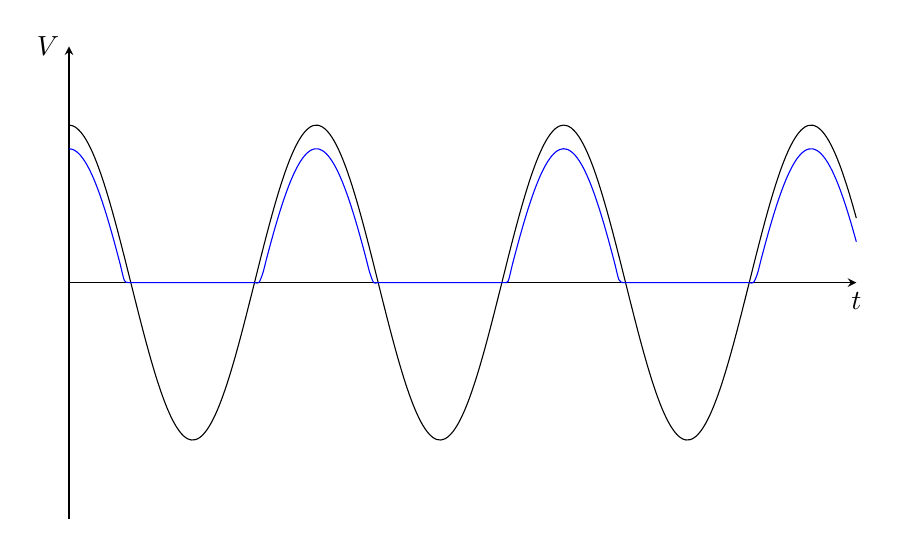
\begin{tikzpicture}
			\draw[-stealth](0,0)--(10,0)node[below]{$t$};
			\draw[-stealth](0,-3)--(0,3)node[left]{$V$};
			\draw[domain=0:10, smooth, samples=200] plot (\x, {2*cos(\x*360/pi)});
			\draw[domain=0:10, smooth, samples=200, blue] plot (\x, {cos(\x*360/pi)-0.15+(cos(\x*360/pi)-0.15)*sign(cos(\x*360/pi)-0.15)});
		\end{tikzpicture}
		\caption{tensione in ingresso (nero) e in uscita (blu) per il raddrizzatore a semionda.}
		\label{fig:raddrsemigraf}
	\end{figure}
	Questo circuito è molto semplice, ma di fatto si utilizza solo la metà della tensione in ingresso.
	\subsubsection{Raddrizzatore a onda intera}
	Questo circuito, chiamato anche raddrizzatore a doppia semionda, permette di trasformata un'onda sinusoidale nel suo modulo. Il circuito è riportato in figura \ref{fig:raddrint}, mentre in figura \ref{fig:raddrintgraf} è riportato un grafico delle tensioni in ingresso e in uscita.
	\begin{figure}[h!]
		\centering
		\begin{circuitikz}
			\draw(2,0)--(0,0)to[sV](0,2.1)to(2,2.1);
			\node at(3, 2.1)[transformer core]{};
			\draw(3.5,2.1)to[diode=$D_1$](7,2.1)to(8,2.1)to[R=$R_L$](8,0)node[ground]{};
			\draw(8.5,2.1)node[anchor=west]{$V\ped{out}$}to[short, o-](8,2.1);
			\draw(3.5,0)to[diode=$D_2$](7,0)to[short, -*](7,2.1);
			\draw(3.5,1.05)--(4.3,1.05)node[ground]{};
		\end{circuitikz}
		\caption{raddrizzatore a onda intera.}
		\label{fig:raddrint}
	\end{figure}
	\begin{figure}[h!]
		\centering
		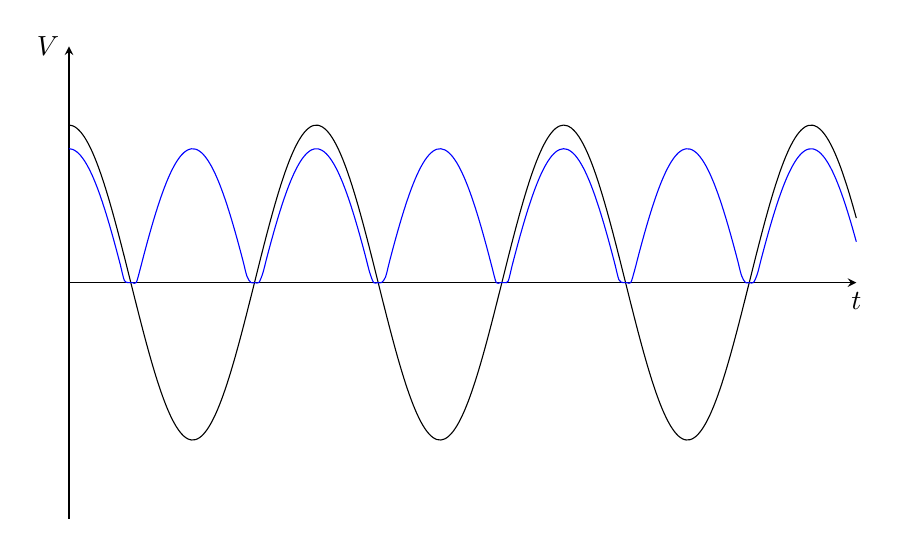
\begin{tikzpicture}
		\draw[-stealth](0,0)--(10,0)node[below]{$t$};
		\draw[-stealth](0,-3)--(0,3)node[left]{$V$};
		\draw[domain=0:10, smooth, samples=200] plot (\x, {2*cos(\x*360/pi)});
		\draw[domain=0:10, smooth, samples=200, blue] plot (\x, {abs(cos(\x*360/pi))-0.15+abs(abs(cos(\x*360/pi))-0.15)});
		\end{tikzpicture}
		\caption{tensione in ingresso (nero) e in uscita (blu) per il raddrizzatore a onda intera.}
		\label{fig:raddrintgraf}
	\end{figure}
	Questo circuito risolve il problema del raddrizzatore a semionda, ma comunque ha degli svantaggi: per realizzare un singolo raddrizzatore occorrono due diodi, ma questi non vengono mai usati contemporaneamente in diretta. Una variante del raddrizzatore a onda intera si ottiene anche con un ponte di diodi, mostrato in figura \ref{fig:pontediodi}.
	\begin{figure}[h!]
		\centering
		\begin{circuitikz}
			\draw(2,0)--(0,0)to[sV](0,2.1)to(2,2.1);
			\node at(3, 2.1)[transformer core]{};
			\draw(4,2.1)to(7,2.1)to(7,1.1)to[diode=$D_1$](8.5,-.6)to(10,-.6)to[R=$R_L$](10,-3)node[ground]{};
			\draw(10.5,-0.6)node[anchor=west]{$V\ped{out}$}to[short, -o](10,-0.6);
			\draw(4,0)to(4,-3)to(7,-3)to(7,-2.1)to[diode](8.5,-0.6);
			\draw(5,-0.6)node[ground]{}to(5.5,-0.6)to[diode](7,1.1);
			\draw(5.5,-0.6)to[diode](7,-2.1);
		\end{circuitikz}
		\caption{raddrizzatore a onda intera con ponte di diodi.}
		\label{fig:pontediodi}
	\end{figure}
	Il circuito può essere ulteriormente complicato aggiungendo in uscita un filtro passa-basso, come mostrato in figura \ref{fig:ripple}. Se supponiamo che sia $R_LC\gg T$, dove $T$ è il periodo dell'onda in ingresso, allora il segnale in uscita è quasi continuo, nel senso che tra un picco e l'altro decresce quasi linearmente come
	\[V(t)\simeq V_0\left(1-\frac{t}{R_LC}\right)\]
	dove $V_0+V_\gamma$ è l'ampiezza del segnale in ingresso. La caduta di tensione $\Delta V$ così ottenuta è detta ripple. Trascurando il tempo in cui il segnale cresce, è
	\[\Delta V\simeq\frac{1}{2fR_LC}\]
	dove $f$ è la frequenza del segnale in ingresso. Viceversa, quando il segnale in uscita cresce riesce a seguire fedelmente il segnale in ingresso: questo è dovuto al fatto che il condensatore si carica dal ponte, mentre si scarica solo su $R_L$. Il segnale in uscita è riportato in figura \ref{fig:ripplegraf}.
	\begin{figure}[h!]
		\centering
		\begin{circuitikz}
			\draw(2,0)--(0,0)to[sV](0,2)to(2,2);
			\draw(2,2.5)to(5,2.5)to(5,-0.5)to(2,-0.5)to(2,2.5);
			\draw(3.5,1)node[]{Rettificatore};
			\draw(5,2)to[R=$R$](7,2)to[C=$C$](7,0)to(5,0);
			\draw(7,2)to(9,2)to[R=$R_L$](9,0)to(7,0)node[ground]{};
			\draw(9.5,2)node[anchor=west]{$V\ped{out}$}to[short,o-](9,2);
		\end{circuitikz}
		\caption{circuito per un segnale quasi continuo.}
		\label{fig:ripple}
	\end{figure}
	\begin{figure}[h!]
		\centering
		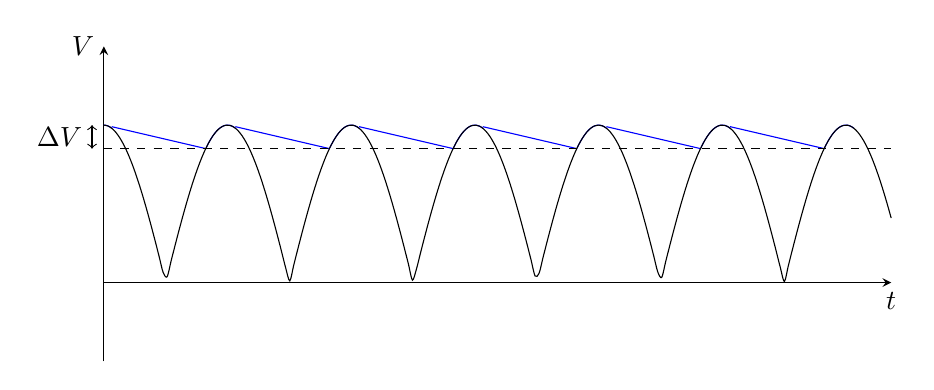
\begin{tikzpicture}
			\draw[-stealth](0,0)--(10,0)node[below]{$t$};
			\draw[-stealth](0,-1)--(0,3)node[left]{$V$};
			\draw[domain=0:0.1, smooth, samples=200, blue] plot (\x, {2*cos(\x*360/pi)});
			\foreach \x in {0,1,...,5}{
				\draw[blue](0.1+\x*pi/2,1.98)--(1.3+\x*pi/2,1.7);
			}
			\draw[blue, domain=(1.3):(0.1+pi/2), smooth, samples=100] plot (\x,{2*abs(cos(\x*360/pi))});
			\draw[blue, domain=(1.3+pi/2):(0.1+pi), smooth, samples=100] plot (\x,{2*abs(cos(\x*360/pi))});
			\draw[blue, domain=(1.3+pi):(0.1+3*pi/2), smooth, samples=100] plot (\x,{2*abs(cos(\x*360/pi))});
			\draw[blue, domain=(1.3+3*pi/2):(0.1+4*pi/2), smooth, samples=100] plot (\x,{2*abs(cos(\x*360/pi))});
			\draw[blue, domain=(1.3+4*pi/2):(0.1+5*pi/2), smooth, samples=100] plot (\x,{2*abs(cos(\x*360/pi))});
			\draw[blue, domain=(1.3+5*pi/2):(0.1+6*pi/2), smooth, samples=100] plot (\x,{2*abs(cos(\x*360/pi))});
			\draw[domain=0:10, smooth, samples=200] plot (\x, {2*abs(cos(\x*360/pi))});
			\draw[dashed](0,1.7)--(10,1.7);
			\draw[<->](-0.15,1.7)--(-0.15,2);
			\node at(-0.15,1.85)[left]{$\Delta V$};
		\end{tikzpicture}
		\caption{tensione in uscita (blu) e all'uscita del rettificatore (nero) per il circuito in figura \ref{fig:ripple}.}
		\label{fig:ripplegraf}
	\end{figure}
	\subsubsection{Rivelatore di picco}
	Il rivelatore di picco si basa sull'idea del circuito precedente ed è mostrato in figura \ref{fig:rivpicco}. Essenzialmente, se in ingresso arriva un picco di tensione (qui rappresentato dal generatore sinusoidale), allora in uscita viene mantenuta la tensione di picco per un tempo di circa $R_LC$. Infatti, quando il diodo è in conduzione il condensatore si carica, mentre quando il diodo è in inversa il condensatore si scarica su $R_L$, ma possiamo aumentare a piacere il tempo di scarica di questo sottocircuito.
	\begin{figure}[h!]
		\centering
		\begin{circuitikz}
			\draw (0,0)node[ground]{}to[sV](0,2)to[diode](2,2)to[C=$C$](2,0)to[short, -*](0,0);
			\draw(2,2)to(4,2)to[R=$R_L$](4,0)to(2,0);
			\draw(4.5,2)node[anchor=west]{$V\ped{out}$}to[short, o-](4,2);
		\end{circuitikz}
		\caption{rivelatore di picco.}
		\label{fig:rivpicco}
	\end{figure}
	\subsubsection{Clamp}
	Il clamp limite la tensione in ingresso ed è mostrato in figura \ref{fig:clamp}. Infatti, se la tensione in ingresso $V$ è maggiore di $-V_\gamma$, allora è $V\ped{out}=V$. Viceversa, se $V<-V_\gamma$ allora è $V\ped{out}=-V_\gamma$, dunque riusciamo a limitare la tensione minima in uscita. La resistenza $R$ viene usata per limitare la corrente che scorre nel circuito quando il diodo è in conduzione, ma è opportuna sceglierla molto piccola rispetto a un'eventuale resistenza di carico $R_L$.
	\begin{figure}[h!]
		\centering
		\begin{circuitikz}
			\draw(0,0)node[ground]{}to(2,0)to[diode](2,2)to[R=$R$](0,2)to[sV](0,0);
			\draw(2.5,2)node[anchor=west]{$V\ped{out}$}to[short, o-*](2,2);
			\draw(2.5,0)to[short, -*](2,0);
		\end{circuitikz}
		\caption{clamp.}
		\label{fig:clamp}
	\end{figure}
	\subsubsection{Doppio clamp}
	Un doppio clamp è un circuito che, come suggerisce il nome, limita la tensione in ingresso sia dall'alto che dal basso. Il circuito è mostrato in figura \ref{fig:doppioclamp} e limita la tensione tra $V_0+V_\gamma$ e $-V_\gamma$.
	\begin{figure}[h!]
		\centering
		\begin{circuitikz}
		\draw(0,0)to(2,0)node[ground]{}to[diode](2,2)to[R=$R$](0,2)to[sV](0,0);
		\draw(2,2)to[diode](2,4)to(2.5,4)to(1.5,4);
		\draw(2,4)node[anchor=south]{$+V_0$};
		\draw(2,2)to[short,*-](4,2)to[R=$R_L$](4,0)to[short,-*](2,0);
		\draw(4.5,2)node[anchor=west]{$V\ped{out}$}to[short,o-](4,2);
		\end{circuitikz}
		\caption{doppio clamp.}
		\label{fig:doppioclamp}
	\end{figure}
	\subsubsection{Clamp con diodi Zener}
	Questo circuito è essenzialmente un doppio clamp, che però sfrutta la tensione di breakdown di due diodi Zener. In tal modo, la tensione è limitata tra $-(V_z+V_\gamma)$ e $V_z+V_\gamma$. Il circuito è riportato in figura \ref{fig:clampzener}.
	\begin{figure}[h!]
		\centering
		\begin{circuitikz}
			\draw(2,2)to[zzD](2,0)to(0,0)node[ground]{}to[sV](0,4)to[R=$R$](2,4);
			\draw(2,2)to[zzD](2,4);
			\draw(2.5,4)node[anchor=west]{$V\ped{out}$}to[short,o-*](2,4);
			\draw(2.5,0)to[short, -*](2,0);
		\end{circuitikz}
		\caption{clamp con diodi Zener.}
		\label{fig:clampzener}
	\end{figure}
	\subsubsection{Duplicatore di tensione}
	Il duplicatore di tensione permette di caricare selettivamente due condensatori messi in serie. Il segnale in uscita ha un'ampiezza che è (circa) il doppio del segnale in ingresso, infatti quando il segnale in ingresso è positivo entrambi i condensatori si caricano. In particolare, è $V_+=-V_=V\ped{in}$, a meno della caduta $V_\gamma$ sul diodo. Quando invece il segnale in ingresso è negativo i diodi non conducono e il segnale si scarica su una resistenza di carico, per semplicità non rappresentata nel circuito. Il duplicatore ha lo svantaggio di dare una tensione in uscita sia positiva ($V_+$) che negativa ($V_-$) rispetto a terra.
	
	\begin{figure}[h!]
		\centering
		\begin{circuitikz}
			\draw(2,0)--(0,0)to[sV](0,2.1)to(2,2.1);
			\node at(3, 2.1)[transformer core]{};
			\draw(4,2.1)to[diode](8,2.1)to[C=$C$](8,0)to[C=$C$](8,-2.1)to[diode](5,-2.1)to(5,2.1);
			\draw(8,1.1)node[above right]{+};
			\draw(8,-0.95)node[above right]{+};
			\draw(4,0)to(4.8,0);
			\draw(5.1,0)to(6.5,0)node[ground]{}to[short, -*](8,0);
			\draw(8.5,2.1)to[short, -*](8,2.1);
			\draw(8.5,-2.1)to[short, -*](8,-2.1);
			\draw(8,2.1)node[anchor=south]{$V_+$};
			\draw(8,-2.1)node[anchor=north]{$V_-$};
		\end{circuitikz}
		\caption{duplicatore di tensione.}
		\label{fig:duptens}
	\end{figure}
	\subsubsection{Duplicatore di tensione positiva}
	Il duplicatore di tensione positiva risolve il problema precedente restituendo un segnale sempre positivo rispetto a terra e di ampiezza doppia rispetto all'ampiezza del segnale in ingresso. Il circuito è riportato in figura \ref{fig:duptenspos}.
	\begin{figure}[h!]
		\centering
		\begin{circuitikz}
			\draw(0,0)node[ground]{}to(2,0)to[diode,-*](2,2)to[C=$C_1$](0,2)to[sV](0,0)node[ground]{};
			\draw(2,2)to[diode](4,2)to[C=$C_2$](4,0)to[short, -*](2,0);
			\draw(4.5,2)node[anchor=west]{$V\ped{out}$}to[short, o-*](4,2);
			\draw(4.5,0)to[short, -*](4,0);
			\draw(1.1,2)node[above right]{+};
			\draw(4,1.1)node[above right]{+};
		\end{circuitikz}
		\caption{duplicatore di tensione positiva.}
		\label{fig:duptenspos}
	\end{figure}
	\clearpage
	\section{Transistor}
	Il diodo è comunque un dispositivo passivo: non è possibile amplificare un segnale. Un elemento non lineare che può amplificare di un fattore notevole un piccolo segnale è il transistor. Chiaramente, la potenza del segnale amplificato proviene da un opportuno circuito di alimentazione del transistor. Nel BJT (bipolar junction transistor) si riesce ad amplificare una corrente. Un BJT consiste essenzialmente in una doppia giunzione, dunque è possibile distinguere in transistor BJT npn e transistor BJT pnp. I simboli circuitali sono riportati in figura \ref{fig:bjt}. 
	\begin{figure}[h!]
		\centering
		\begin{circuitikz}
			\draw(0,0)node[npn] (npn){}
				(npn.base)node[anchor=east]{$B$}
				(npn.collector)node[anchor=south]{$C$}
				(npn.emitter)node[anchor=north]{$E$};
			
			\draw(3,0)node[pnp] (pnp){}
			(pnp.base)node[anchor=east]{$B$}
			(pnp.collector)node[anchor=north]{$C$}
			(pnp.emitter)node[anchor=south]{$E$};
		\end{circuitikz}
		\caption{transistor npn (sinistra) e pnp (destra).}
		\label{fig:bjt}
	\end{figure}
	I terminali $C$, $B$ ed $E$ sono detti rispettivamente collettore, base ed emettitore. Tipicamente, un BJT viene utilizzato con la giunzione $BE$ polarizzata direttamente e con la giunzione $BC$ polarizzata inversamente. La corrente $I_B$ che entra nella base permette di controlla in maniera molto efficace la corrente attraverso gli altri due terminali. Come suggerisce il nome, i portatori di carica sono emessi dall'emettitore e raccolti dal collettore. Questo è possibile perchè tutto il dispositivo è un monocristallo e la base è, di solito, molto sottile e poco drogata, quindi il comportamento di un transistor è ben diverso da quello di due diodi in serie. Inoltre, per un BJT npn i portatori sono elettroni, mentre per un BJT pnp i portatori sono lacune. D'ora in poi ci limitiamo ai BJT npn, dato che lo studio dei BJT pnp è del tutto analogo, a parte qualche cambio di segno.
	
	Vediamo ora il funzionamento specifico di un BJT npn: siano $I_B, I_C, I_E$ rispettivamente le correnti di base, di collettore e di emettitore. Prendiamo tali correnti come positive se entrano nel dispositivo. In tal modo, la legge di Kirkhhoff sulle correnti è
	\[I_B+I_C+I_E=0\]
	Sia inoltre $V_{ij}=V_i-V_j$ per $i,j=B,C,E$. Ad esempio, $V_{CE}$ è la d.d.p. tra collettore ed emettitore, ed è positiva se $V_C>V_E$. Questa notazione è particolarmente utile nei calcoli perchè
	\[V_{ij}=-V_{ji},\qquad\qquad V_{ij}-V_{jk}=V_{ik}\]Si ha\footnote{Ma non so perchè, mannaggia agli sperimentali.}
	\[I_C=I_S\left(e^{V_{BE}/V_T}-e^{V_{BC}/V_T}\right)\]
	
	Normalmente è $V_C>V_B>V_E$, in accordo con quanto detto prima sulle polarizzazioni delle due giunzioni. Questo regime è detto zona attiva, e in tal caso è
	\[I_C\simeq I_Se^{V_{BE}/V_T}\simeq h_{FE}I_B,\qquad\qquad V_{BE}\simeq 0.6-0.7\,\mathrm{V}\]
	Tipicamente è $I_B\simeq1-10\,\mu$A. $I_C$ è in genere grande rispetto a $I_B$, ossia $h_{FE}$ (chiamato large signal current gain) è molto grande, intorno a 100. Tipicamente $I_C\simeq 1$ mA, dunque si trova anche $I_E\simeq-I_C$. Più precisamente, posto
	\[I_C=-\alpha_FI_E\]
	dove $\alpha_F$ rappresenta l'efficienza di raccolta del collettore degli elettroni emessi dall'emettitore, allora si ha
	\[I_C=\frac{\alpha_F}{1-\alpha_F}I_B\]
	Questo determina $h_{FE}$, ma dato che la base è sottile e poco drogata ci aspettiamo $\alpha_F\simeq1$. Questo fa variare notevolmente $h_{FE}$ da dispositivo a dispositivo.
	
	Supponiamo ora $V_C<V_B<V_E$. Questo regime è detto reverse active, dato che consiste di fatto in uno scambio di ruoli tra collettore ed emettitore. Per motivi costruttivi, questo regime è meno efficace di quello attivo e per questo non viene usato: il drogaggio e le dimensioni di collettore ed emettitore sono diversi, dunque se introduciamo il coefficiente
	\[I_E=-\alpha_RI_C\]
	analogo al coefficiente $\alpha_F$, si trova
	\[I_E=\frac{\alpha_R}{1-\alpha_R}I_B\]
	In questo caso però non è $\alpha_R\simeq1$.
	
	Supponiamo ora $V_B<V_C$ e $V_B<V_E$. In tal caso entrambe le giunzioni sono polarizzate direttamente, quindi tale regime è detto saturazione. Si ha allora
	\[I_C=I_Se^{V_{BE}/V_T}\left(1-e^{-V_{CE}/V_T}\right)\simeq h_{FE}I_B\left(1-e^{-V_{CE}/V_T}\right)\]
	Se poi $V_{CE}$ è piccola rispetto alla tensione termica allora
	\[I_C\simeq\frac{h_{FE}V_{CE}}{V_T}I_B\]
	Tipicamente $V_{CE}\simeq0.2$ V, quindi la condizione di piccolezza non sembra verificata. Ma gli sperimentali sono sperimentali.
	
	Infine, per $V_B>V_C$ e $V_B>V_E$ entrambe le giunzioni sono polarizzate inversamente. Questo regime è detto interdizione e in questo caso tutte le correnti sono approssimativamente nulle. I possibili regimi sono schematizzati in figura \ref{fig:regbjt}.
	\begin{figure}[h!]
		\centering
		\begin{tikzpicture}
			\draw[-stealth](-4,0)--(4,0)node[below]{$V_{BE}$};
			\draw[-stealth](0,-3)--(0,3)node[left]{$V_{BC}$};
			\node at(2,2){Saturazione};
			\node at(2,-2){Zona attiva};
			\node at(-2,-2){Interdizione};
			\node at(-2,2){Reverse active};
		\end{tikzpicture}
		\caption{diversi regimi di operazione di un transistor.}
		\label{fig:regbjt}
	\end{figure}
	
	Un altro grafico molto utilizzato è quello delle caratteristiche di uscita, in cui si riporta $I_C$ in funzione di $V_{CE}$. In questo grafico si riportano in realtà diverse curve di uscita, ciascuna a un dato valore di $I_B$. Sono riportate in figura \ref{fig:uscitabjt}. La saturazione, come abbiamo visto, corrisponde a piccoli valori di $V_{CE}$, quindi si trova nella parte a sinistra del grafico. L'interdizione corrisponde a $I_C\simeq 0$, dunque corrisponde alla parte in basso del grafico. 
	\begin{figure}[h!]
		\centering
		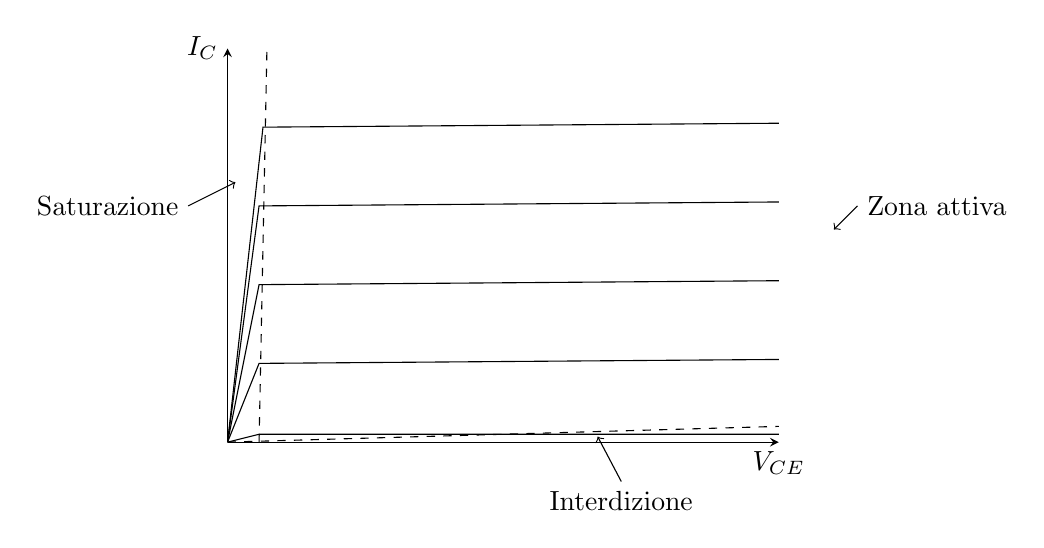
\begin{tikzpicture}
		\draw[-stealth](0,0)--(0,5)node[left]{$I_{C}$};
		\draw[-stealth](0,0)--(7,0)node[below]{$V_{CE}$};
		\draw[dashed](0.4,0)--(0.5,5);
		\draw[dashed](0,0)--(7,0.2);
		\node at(5,-0.5)[below]{Interdizione};
		\draw[->](5,-0.5)--(4.7,0.07);
		\node at(8,3)[right]{Zona attiva};
		\node at(-0.5,3)[left]{Saturazione};
		\draw[->](-0.5,3)--(0.1,3.3);
		\draw[->](8,3)--(7.7,2.7);
		\draw(0,0)--(0.4,1)--(7,1.05);
		\draw(0,0)--(0.4,0.1)--(7,0.1);
		\draw(0,0)--(0.4,2)--(7,2.05);
		\draw(0,0)--(0.4,3)--(7,3.05);
		\draw(0,0)--(0.45,4)--(7,4.05);
		\end{tikzpicture}
		\caption{caratteristiche di uscita.}
		\label{fig:uscitabjt}
	\end{figure}
	Vediamo ora alcuni utilizzi di base di un transistor.
	\subsection{Interruttore}
	Consideriamo il circuito in figura \ref{fig:transinterr}. Il simbolo che ricorda da vicino un prodotto tensoriale è il simbolo circuitale per una lampadina.
	\begin{figure}[h!]
		\centering
		\begin{circuitikz}
			\draw(3,3)to(0,3)to[nos](0,2)to[R=${R=}10\,\mathrm{k}\Omega$](0,0)to(2.2,0);
			\draw(3,3)to[lamp](3,0.5);
			\draw(3,0)node[npn]{};
			\draw(3,-0.5)node[ground]{};
			\draw(3.5,3)node[anchor=west]{$V\ped{in}=10\,\mathrm{V}$}to[short, o-*](3,3);
		\end{circuitikz}
		\caption{interrutore.}
		\label{fig:transinterr}
	\end{figure}

	\noindent La lampadina può essere modellizzata come una resistenza di circa $R_L\simeq10\,\Omega$. Chiaramente se l'interrutore è aperto $I_B=0$, dunque anche $I_C=0$ e la lampadina è spenta. Viceversa, se l'interrutore è chiuso allora è
	\[V\ped{in}=R_LI_C+V_{CE}\]
	Questa equazione, rappresentata graficamente sul piano $I_C-V_{CE}$, rappresenta la retta di carico. Il punto di lavoro è determinato dall'intersezione di tale retta con la curva di collettore corrispondente alla corrente $I_B$ che scorre nella base. Questa può essere determinata facilmente da
	\[V\ped{in}=RI_B+V_{BE}\]
	Se siamo in zona attiva o in saturazione la giunzione $BE$ è polarizzata direttamente, quindi $V_{BE}\simeq0.6-0.7$ V. Così facendo si trova
	\[I_B\simeq930\,\mu\mathrm{A}\]
	\subsection{Emitter follower}
	L'emitter follower è il circuito rappresentato in figura \ref{fig:emitterfollower}. In genere viene utilizzato per segnali in ingresso $V\ped{in}$ oscillanti e piccoli rispetto alle tensioni di polarizzazione del transistor. Queste tensioni continue definiscono il punto di lavoro (o di quiescenza) del circuito. Per segnali oscillanti come quello in ingresso i coefficienti che abbiamo introdotto in precedenza possono cambiare. Per distinguere dalle grandezze continue, indicheremo le grandezze oscillanti con lettere minuscole. Ad esempio, possiamo introdurre lo small signal current gain $h_{fe}$, definito da
	\[i_C=h_{fe}i_B\]
	e in generale $h_{fe}\neq h_{FE}$, anche se il loro valore è abbastanza simile. Più in generale, possiamo linearizzare tutte le grandezze oscillanti intorno al punto di lavoro, se queste hanno ampiezza piccola e il punto di lavoro si trova nella zona attiva. Questa approssimazione è nota come modello a parametri $h$.
	\begin{figure}[h!]
		\centering
		\begin{circuitikz}
			\draw(0,0)node[npn]{};
			\draw(0.5,-0.5)node[anchor=west]{$v\ped{out}$}to[short,o-](0,-0.5)to[R=$R_E$](0,-2.5)node[ground]{};
			\draw(-1,0)node[anchor=east]{$v\ped{in}$}to(-0.5,0);
		\end{circuitikz}
		\caption{emitter follower.}
		\label{fig:emitterfollower}
	\end{figure}
	Se il transistor è in zona attiva, allora si trova semplicemente
	\[v\ped{out}=v\ped{in}-V_{BE}\simeq v\ped{in}-0.7\,\mathrm{V}\]
	da cui il nome emitter follower. Il circuito viene utilizzato come adattore di impedenza, perchè $Z\ped{out}\ll Z\ped{in}$. Queste impedenze vanno in realtà calcolate come impedenze dinamiche, dato che siamo interessati a segnali oscillanti. Ad esempio, è
	\[Z\ped{in}=\frac{\d v\ped{in}}{\d i\ped{in}}\]
	anche se gli elettrotecnici in genere scrivono questa definizione come rapporto di piccole variazioni di tensione e corrente, ovvero
	\[Z\ped{in}=\frac{\Delta v\ped{in}}{\Delta i\ped{in}}\]
	Consideriamo ora l'emitter follower e calcoliamo le due impedenze: la corrente in ingresso è $i_B$, legata a $i_E$ da
	\[i_E=i_B(h_{fe}+1)\]
	dove abbiamo posto $i_E>0$ se è uscente dall'emettitore. Per le variazioni di corrente è allora
	\[\Delta i_E=\Delta i_B(h_{fe}+1)\]
	Per le variazioni di tensione si ha chiaramente
	\[\Delta v\ped{in}=\Delta v\ped{out}\]
	e d'altro canto è
	\[\Delta v\ped{out}=R_E\Delta i_{E}\]
	Infine si trova
	\[Z\ped{in}=R_E(h_{fe}+1)\]
	Dunque l'impedenza di ingresso è grande (rispetto a $R_E$).
	Per calcolare l'impedenza di uscita dobbiamo ricordare che
	\[Z\ped{out}=\frac{\d v\ped{out}^{\text{ap}}}{\d i\ped{out}^{\text{cc}}}\]
	Immaginiamo di aggiungere una resistenza $R_S$ prima dell'ingresso, come mostrato in figura \ref{fig:bjtzout}.
	\begin{figure}[h!]
		\centering
		\begin{circuitikz}
			\draw(0,0)node[npn]{};
			\draw(0.5,-0.5)node[anchor=west]{$v\ped{out}$}to[short,o-](0,-0.5)to[R=$R_E$](0,-2.5)node[ground]{};
			\draw(-3,0)node[anchor=east]{$v\ped{in}$}to(-2.5,0)to[R=$R_S$](-0.5,0);
		\end{circuitikz}
		\caption{emitter follower.}
		\label{fig:bjtzout}
	\end{figure}
	Per piccole variazioni del segnale in ingresso, è
	\[\Delta v\ped{out}^{\text{ap}}=\Delta v\ped{in},\qquad\qquad\Delta i\ped{out}^{\text{cc}}=\Delta i_E\]
	e dunque
	\[Z\ped{out}=\frac{R_S}{h_{fe}+1}\]
	Questa impedenza può quindi essere classificata come piccola. Il guadagno in tensione è, come già visto, circa unitario.
	
	Questo studio è corretto se, come già detto, è presente un circuito di polarizzazione che mantenga le giuste tensioni (continue) alla base, al collettore e all'emettitore. Un emitter follower vero e proprio è quindi più complicato di quello che abbiamo rappresentato, ed è riportato in figura \ref{fig:realemitterfollower}.
	\begin{figure}[h!]
		\centering
		\begin{circuitikz}
			\draw(3,0)node[npn]{};
			\draw(-3,0)node[anchor=east]{$v\ped{in}$}to[short,o-](-2.5,0)to[C=$C_1$](0,0);
			\draw(3.5,2)node[anchor=west]{$V_0$}to[short,o-](3,2)to(0,2)to[R=$R_1$](0,0)to[R=$R_2$](0,-2.5)to(1.5,-2.5)node[ground]{}to(3,-2.5)to[R=$R_E$](3,-0.5)to[C=$C_2$](4.5,-0.5)to[short,-o](5,-0.5)node[anchor=west]{$v\ped{out}$};
			\draw(3,2)to(3,0.5);
			\draw(0,0)to[short, *-](2.5,0);
		\end{circuitikz}
		\caption{emitter follower.}
		\label{fig:realemitterfollower}
	\end{figure}
	I condensatori servono semplicemente a disaccoppiare le tensioni continue dall'ingresso e dall'uscita dei segnali oscillanti, ossia sono usati come dei passa-alto.
	\subsection{Modello a piccolo segnale}
	Studiamo più in dettaglio il comportamento di un transistor per piccoli segnali. Come già detto, una buona approssimazione consiste nel linearizzare il dispositivo il più possibile. Questo significa ad esempio che, in regime attivo, un transistor è, in prima approssimazione, equivalente al circuito in figura \ref{fig:transpicc}.
	\begin{figure}[h!]
		\centering
		\begin{circuitikz}
			\draw(0,0)to(2,0)to(2,-2)to(4,-2)to[ioosource=$h_{fe}i_B$](4,0)to(6,0);
			\draw[-latex](0.5,0.5)to(1.5,0.5);
			\draw(1,0.5)node[anchor=south]{$i_B$};
			\draw[-latex](5.5,0.5)to(4.5,0.5);
			\draw(5,0.5)node[anchor=south]{$i_C$};
			\draw(3,-2)to(3,-2.5)node[anchor=north]{$E$};
			\draw(2,0)node[anchor=south]{$B$};
			\draw(4,0)node[anchor=south]{$C$};
		\end{circuitikz}
		\caption{circuito equivalente a un transistor.}
		\label{fig:transpicc}
	\end{figure}

	\noindent Questo modello però è ancora troppo rozzo. Ad esempio, non tiene conto della resistenza dinamica della giunzione $BE$, che è con buona approssimazione
	\[r_{BE}=\frac{i_B}{V_T}\]
	Questa resistenza si può introdurre nel modello attraverso il parametro $h_{ie}\simeq 2\,\mathrm{k}\Omega$, che di fatto coincide con $r_{BE}$. Il circuito va allora modificato con quello in figura \ref{fig:transpicchie}.
	\begin{figure}[h!]
		\centering
		\begin{circuitikz}
			\draw(0,0)to(2,0)to[R=$h_{ie}$](2,-2)to(4,-2)to[ioosource=$h_{fe}i_B$](4,0)to(6,0);
			\draw[-latex](0.5,0.5)to(1.5,0.5);
			\draw(1,0.5)node[anchor=south]{$i_B$};
			\draw[-latex](5.5,0.5)to(4.5,0.5);
			\draw(5,0.5)node[anchor=south]{$i_C$};
			\draw(3,-2)to(3,-2.5)node[anchor=north]{$E$};
			\draw(2,0)node[anchor=south]{$B$};
			\draw(4,0)node[anchor=south]{$C$};
		\end{circuitikz}
		\caption{circuito equivalente a un transistor, con resistenza dinamica.}
		\label{fig:transpicchie}
	\end{figure}
	\subsubsection{Effetto Early}
	Il modello lineare è ancora imperfetto, soprattutto per grandi valori di $V_{CE}$. In queste condizioni infatti la giunzione $BC$ diventa più svuotata, in particolare si riduce lo spessore della base. Ci aspettiamo quindi che $I_C$ aumenti. Effettivamente, le curve di collettore in figura \ref{fig:uscitabjt} non sono rette orizzontali, ma hanno una piccola  pendenza positiva. L'intercetta di tali rette è la tensione di Early $-V\ped{Early}$. In tal caso quindi si ha
	\[i_C=h_{fe}i_B+h_{oe}v_C\]
	dove $h_{oe}\simeq10^{-5}$ S è un nuovo parametro del modello, con le dimensioni di una conduttanza\footnote{Per gli amici, l'inverso di una resistenza.}. Inoltre, sempre per l'effetto Early la corrente in base $i_B$ si riduce. Questa riduzione viene modellizzata dal parametro adimensionale $h_{re}\simeq10^{4}$, definito da
	\[v_{BE}=h_{ie}i_B+h_{re}v_{CE}\]
	e dunque in definitiva il circuito equivalente a un transistor in regime attivo nel modello a piccolo segnale è quello di figura \ref{fig:transpiccolo}.
	\begin{figure}[h!]
		\centering
		\begin{circuitikz}
			\draw(-2,0)to(0,0)to[R=$h_{ie}$](2,0)to[american voltage source, l_=$h_{re}v_{CE}$](2,-2)to(4,-2)to[ioosource=$h_{fe}i_B$](4,0)to(8,0);
			\draw[-latex](-1.5,0.5)to(-.5,0.5);
			\draw(-1,0.5)node[anchor=south]{$i_B$};
			\draw[-latex](7.5,0.5)to(6.5,0.5);
			\draw(7,0.5)node[anchor=south]{$i_C$};
			\draw(3,-2)to(3,-2.5)node[anchor=north]{$E$};
			\draw(-2,0)node[anchor=south]{$B$};
			\draw(8,0)node[anchor=south]{$C$};
			\draw(4,-2)to(6,-2)to[R=$h_{oe}^{-1}$](6,0);
		\end{circuitikz}
		\caption{circuito equivalente a un transistor, con resistenza dinamica.}
		\label{fig:transpiccolo}
	\end{figure}
	Infine, in tabella \ref{tab:transpiccolo} sono riportati i diversi parametri introdotti.
	\begin{table}[h!]
		\centering
		\begin{tabular}{|c| c| c| c| c|}
			\hline
			Parametro&Dimensioni&Valore tipico&Utilizzo&Formula\\\hline
			$h_{fe}$&adimensionale&100-1000&guadagno in corrente&$i_C=h_{fe}i_B$\\$h_{ie}$&resistenza&1-10 k$\Omega$&resistenza giunzione $BE$&$v_{BE}=h_{ie}i_B$\\$h_{re}$&adimensionale&$10^{-4}$&diminuzione di $i_B$ per effetto Early&$v_{BE}=h_{ie}i_B+h_{re}v_{CE}$\\
			$h_{oe}$&conduttanza&$10^{-5}$ S&aumento di $i_C$ per effetto Early&$i_C=h_{fe}i_B+h_{oe}v_{CE}$\\
			\hline
		\end{tabular}
		\caption{parametri per la linearizzazione di un transistor.}
		\label{tab:transpiccolo}
	\end{table}
	\subsection{Circuiti con transistor}
	\subsubsection{Circuito\sf{NOT}}
	Il \sf{NOT} è un circuito che, dato in ingresso un segnale a livello "alto", ha in uscita un segnale a livello "basso" e viceversa. Questo significa che, grosso modo, vogliamo una funzione di risposta come quella di figura \ref{fig:notrisp}
	\begin{figure}[h!]
		\centering
		\begin{tikzpicture}
			\draw[-stealth](0,0)--(6,0)node[below]{$V\ped{in}$};
			\draw[-stealth](0,0)to(0,5)node[left]{$V\ped{out}$};
			\draw(0,4)--(3,4)--(4,1)--(6,1);
			\draw[dotted](3,0)node[below]{$V{i,L}$}--(3,4)--(0,4)node[left]{$V_{o,H}$};
			\draw[dotted](4,0)node[below]{$V_{i,H}$}--(4,1)--(0,1)node[left]{$V_{o,L}$};
		\end{tikzpicture}
		\caption{funzione di risposta di un \sf{NOT}.}
		\label{fig:notrisp}
	\end{figure}

	\noindent A rigore dovremmo definire meglio cosa significa tensione alta o bassa. Lo faremo in dettaglio nella sezione di elettronica digitale. Il circuito è riportato in figura \ref{fig:notbjt}.
	\begin{figure}[h!]
		\centering
		\begin{circuitikz}
			\draw(-0.5,0)node[anchor=east]{$V\ped{in}$}to[short,o-](0,0)to[R=${R_1=}15\,\mathrm{k}\Omega$](2,0)to[R, l_=${R_2=}100\,\mathrm{k}\Omega$](2,-2);
			\draw(2,0)to[short, *-](3,0);
			\draw(3.5,0)node[npn]{};
			\draw(3.5,-0.5)to(3.5,-2)node[ground]{};
			\draw(-0.5,-2)to[short,o-o](5,-2);
			\draw(4.5,0.5)node[anchor=west]{$V\ped{out}$}to[short, o-*](3.5,0.5)to[R=${R_C=}2.2\,\mathrm{k}\Omega$](3.5,2.5)to(3,2.5)to(4,2.5);
			\draw(4.5,2.5)node[anchor=south]{$V_C=5\,\mathrm{V}$};
		\end{circuitikz}
		\caption{circuito \sf{NOT} con transistor.}
		\label{fig:notbjt}
	\end{figure}
	
	\noindent Se $V\ped{in}\simeq0$, cioè se il segnale in ingresso è basso, allora il transistor è interdetto. Questo significa che non scorre corrente attraverso $R_C$, e dunque $V\ped{out}\simeq V_C=5$ V, cioè il segnali in uscita è alto. Per quantificare il livello basso, basta trovare per quali valori di $V\ped{in}$ il transistor rimane interdetto: ciò accade per $V_{BE}\leq0.7$ V, ma se $I_B=0$ allora è
	\[V_{BE}=V\ped{in}\frac{1}{1+\dfrac{R_1}{R_2}}\]
	Dunque il transistor rimane in interdizione fino a $V\ped{in}\simeq 0.8$ V. Viceversa, per $V\ped{in}$ abbiamo una corrente di base
	\[I_B=\frac{V\ped{in}-V_{BE}}{R_1}=\frac{V\ped{in}}{R_1}-50\,\mu\mathrm{A}\]
	Per $V\ped{in}$ non troppo grande il transistor è in regime attivo, ossia $I_C=h_{FE}I_B$. Questo è vero fino a quando non si ha $V_{CE}\simeq0.2$ V. Infatti, in tale condizione il transistor va in saturazione. Questo accade quando
	\[R_CI_C^{\text {sat}}=V_C-0.2\,\mathrm{V}\]
	e dunque corrisponde a una tensione di ingresso
	\[V\ped{in}^{\text{sat}}=R_1\left(\frac{V_C-0.2\,\mathrm{V}}{h_{FE}R_C}+50\,\mu\mathrm{A}\right)\simeq1.1\,\mathrm{V}\]
	Allora se il segnale in ingresso è alto, il che tipicamente significa $V\ped{in}=5$ V, il transistor è in saturazione. In tal caso è $V\ped{out}=V_{CE}\simeq0.2$ V, cioè il segnale in uscita è basso. Si noti che per $V\ped{in}=5$ V è $I_B=280\,\mu$A, quindi il transistor è "molto" saturato. Questo pone delle limitazione nell'usare questo circuito per segnali che variano nel tempo. La ragione principale è il ritardo nel segnale in uscita, dovuto al tempo impiegato dal transistor a passare da saturazione a interdizione e viceversa. Un grafico di tensioni in ingresso e in uscita è riportato in figura \ref{fig:notbjtgraf}.
	\begin{figure}[h!]
		\centering
		\begin{tikzpicture}
			\draw[-stealth](0,-4)--(0,-0.5)node[left]{$V\ped{out}$};
			\draw[-stealth](0,0.5)--(0,4)node[left]{$V\ped{in}$};
			\draw[-stealth](0,-4)--(7,-4)node[below]{$t$};
			\draw[-stealth](0,0.5)--(7,0.5)node[below]{$t$};
			\draw(0,3)--(3,3)--(3,1)--(5,1)--(5,3)--(7,3);
			\draw[dotted](3,1)--(3,-4);
			\draw[dotted](5,1)--(5,-4);
			\draw(0,-3.5)--(3.4,-3.5)--(3.8,-1)--(5.2,-1)--(5.6,-3.5)--(7,-3.5);
		\end{tikzpicture}
		\caption{tensioni in ingresso e in uscita in funzione del tempo.}
		\label{fig:notbjtgraf}
	\end{figure}
	\subsubsection{Amplificatori BJT}
	Abbiamo già visto un amplificatore con un transistor: l'emitter follower. Questo circuito è anche detto common collector. Un altro circuito possibile è quello a common emitter, in cui essenzialmente si cambia solo il punto da cui viene prelevato il segnale in ingresso. I due circuiti sono riportati in figura \ref{fig:bjtcommon}
		\begin{figure}[h!]
		\centering
		\begin{circuitikz}
			\draw(3,0)node[npn]{};
			\draw(-2.5,0)to[C=$C_1$](0,0);
			\draw(3.5,2.5)node[anchor=west]{$V_{CC}$}to[short,o-](3,2.5)to(0,2.5)to[R=$R_1$](0,0)to[R=$R_2$](0,-2.5)node[ground]{}to(3,-2.5)to[R=$R_E$](3,-0.5)to[C, l_=$C_3$](4.5,-0.5)to[short,-o](5,-0.5)node[anchor=west]{$v\ped{out}^{\text{cc}}$};
			\draw(3,2.5)to[R, l_=$R_C$](3,0.5);
			\draw(3,0.5)to[C, l=$C_2$](4.5,0.5)to[short,-o](5,0.5)node[anchor=west]{$v\ped{out}^{\text{ce}}$};
			\draw(0,0)to[short, *-](2.5,0);
			\draw(0,-2.5)to(-2.5,-2.5)to[sV=$v\ped{in}$](-2.5,0);
		\end{circuitikz}
		\caption{common emitter e common collector.}
		\label{fig:bjtcommon}
	\end{figure}
	Il circuito linearizzato è in figura \ref{fig:bjtcommonlin}. Si noti che per segnali oscillanti possiamo non mettere i condensatori. Inoltre, $V_{CC}$ viene sostituita da una messa a terra perchè è una tensione costante. Abbiamo anche trascurato, per semplicità, l'effetto Early.
	\begin{figure}[h!]
		\centering
		\begin{circuitikz}
			\draw(-2,-2)to[sV=$v\ped{in}$](-2,0)to[short, -*](0,0)to[short, -*](2,0)to[short, -*](3,0)node[anchor=south]{$B$}to(4,0)to[R=$h_{ie}$](4,-2)to[short, -*](5,-2)node[anchor=south]{$E$}to(6,-2)to[ioosource=$h_{fe}i_B$](6,0)to[short,-*](7,0)node[anchor=south]{$C$}to(8,0)to[R=$R_C$](8,-5)node[ground]{};
			\draw(0,-2)node[ground]{}to[R=$R_2$](0,0);
			\draw(-2,-2)to(2,-2)to[R=$R_1$](2,0);
			\draw(8,-5)to(5,-5)to[R=$R_E$](5,-2);
			\draw(7.5,1.5)node[anchor=south]{$v\ped{out}^{\text {ce}}$}to[short,o-](7.5,0);
			\draw(6.5,-2.5)node[anchor=west]{$v\ped{out}^{\text {cc}}$}to[short,o-](5,-2.5);
		\end{circuitikz}
		\caption{amplificatori BJT in approssimazione lineare.}
		\label{fig:bjtcommonlin}
	\end{figure}
	Calcoliamo le impedenze di ingresso e di uscita e il guadagno nei due casi. Ovviamente è $v_B=v\ped{in}$, mentre le tensioni in uscita sono
	\[v\ped{out}^{\text {cc}}=i_ER_E,\qquad\qquad v\ped{out}^{\text {ce}}=-i_CR_C\]
	avendo posto $i_C>0$ se la corrente di collettore entra nel transistor e $i_E>0$ se la corrente di emettitore esce dal transistor. Utilizzando $h_{fe}$ si ha anche
	\[v\ped{out}^{\text {cc}}=(h_{fe}+1)i_BR_E,\qquad\qquad v\ped{out}^{\text {ce}}=h_{fe}i_BR_C\]
	D'altro canto è
	\[v_B=v_E+i_Bh_{ie}\]
	dunque si trova
	\begin{align*}A_V^{\text {cc}}&=\frac{v_E}{v_B}=\frac{(h_{fe}+1)R_E}{(h_{fe}+1)R_E+h_{ie}}\\A_V^{\text {ce}}&=\frac{v_C}{v_B}=-\frac{h_{fe}R_C}{(h_{fe}+1)R_E+h_{ie}}\end{align*}
	L'impedenza di ingresso è
	\[Z\ped{in}=\frac{v\ped{in}}{i\ped{in}}\]
	ma $i\ped{in}\neq i_B$. Piuttosto, si trova facilmente
	\[i\ped{in}=i_B+\frac{v\ped{in}}{R_1}+\frac{v\ped{in}}{R_2}\]
	Dunque l'impedenza in ingresso è semplicemente il parallelo tra $R_1$, $R_2$ e $h_{ie}+(h_{fe}+1)R_E$, in entrambi i tipi di amplificatore. La situazione cambia per le impedenze di uscita. Per il common emitter si trova
	\[Z\ped{out}=R_C\]
	Mentre per il common collector
	\[Z\ped{out}=\frac{Z_S+h_{ie}}{h_{fe}}\]
	dove $Z_S$ è l'impedenza della sorgente.%QUESTA PARTE ANDRA' RIVISTA ANCHE DAGLI APPUNTI DI FORTI
	\clearpage
	\section{OpAmp}
	Un amplificatore a due ingressi, lineare e differenziale è un circuito in cui il segnale in uscita è (idealmente) proporzionale alla differenza tra i due segnali in ingresso. Più realisticamente, possiamo assumere una relazione lineare tra ingressi e uscita del tipo
	\[V\ped{out}=A_1V\ped{in,1}+A_2V\ped{in,2}=A_d\left(V_d+\frac{A_c}{A_d}V_c\right)\]
	dove si è posto
	\[A_c=A_1+A_2,\qquad\qquad A_d=\frac{A_1-A_2}{2},\qquad\qquad V_c=\frac{V_1+V_2}{2},\qquad\qquad V_d=V_1-V_2\]
	$A_c$ è detta amplificazione di modo comune, $A_d$ amplificazione di modo differenziale o open loop gain. Un amplificatore operazionale (OpAmp) è un circuito che in una stretta regione di $V_d$ si comporta come un amplificatore differenziale. In un OpAmp ideale è $A_c=0$. In un modello realistico il parametro
	\[\rho=\frac{A_d}{A_c}\]
	è detto fattore di reiezione del modo comune e tipicamente $\rho\simeq10^5$, mentre $A_d\simeq10^5-10^6$. Il simbolo circuitale di un OpAmp è riportato in figura \ref{fig:opamp}.
	\begin{figure}[h!]
		\centering
		\begin{circuitikz}
			\draw(0,0)node[op amp]{};
			\draw(-1.5,0.49)node[anchor=east]{$V\ped{in,2}$}to[short,o-](-1,0.49);
			\draw(-1.5,-0.49)node[anchor=east]{$V\ped{in,1}$}to[short,o-](-1,-0.49);
			\draw(1.5,0)node[anchor=west]{$V\ped{out}$}to[short,o-](1,0);
		\end{circuitikz}
		\caption{simbolo circuitale di un OpAmp.}
		\label{fig:opamp}
	\end{figure}
	Non entreremo nei dettagli costruttivi di un OpAmp, ci basta solo sapere che una buona modellizzazione consiste nel collegare i due ingressi con una resistenza $R\ped{in}$ molto grande, mentre l'uscita è collegata alla serie di una resistenza $R\ped{out}$ e di un generatore di tensione $A_dV_d$. L'OpAmp ideale consiste poi nel prendere i limiti $R\ped{in}\to\infty$, $\rho\to0$. $R\ped{out}\to0$, $A_d\to+\infty$.
	Per il suo funzionamento l'OpAmp ha bisogno di due tensioni di alimentazione $V_{EE}$ e $V_{CC}$, per semplicità non rappresentate. Tipicamente $V_{EE}<0<V_{CC}$. Queste rappresentano anche le tensioni a cui satura il segnale in uscita se $V\ped{in,1}-V\ped{in,2}$ è troppo grande. Visto il valore tipico di $A_d$ e dato che tipicamente $V_{CC}=-V_{EE}=15$ V, "troppo grande" significa $|V\ped{in,1}-V\ped{in,2}|\simeq150\,\mu $V. Di fatto quindi è possibile rappresentare la funzione di risposta dell'OpAmp come un gradino, e l'OpAmp stesso può essere efficacemente utilizzato come discriminatore. La funzione di risposta è riportata in figura \ref{fig:rispostaopamp}.
	\begin{figure}[h!]
		\centering
		\begin{tikzpicture}
			\draw[-stealth](0,-4)--(0,4)node[left]{$V\ped{out}$};
			\draw[-stealth](-7,0)--(7,0)node[below]{$V_d$};
			\draw(-7,-3)--(-2,-3)--(2,3)--(7,3);
			\draw[dotted](-2,-3)--(0,-3)node[right]{$V_{EE}$};
			\draw[dotted](2,3)--(0,3)node[left]{$V_{CC}$};
			\draw[dotted](2,3)--(2,-4);
			\draw[dotted](-2,0)--(-2,-4);
			\draw[<->](-2,-4.1)--(2,-4.1);
			\node at(0,-4.1)[below]{$\Delta V\simeq 300\,\mu\mathrm{V}$};
		\end{tikzpicture}
		\caption{funzione di risposta di un OpAmp.}
		\label{fig:rispostaopamp}
	\end{figure}	
	L'OpAmp può anche essere usato come amplificatore, ma in tal caso è necessario mantenerlo nel regime lineare: questo può essere ottenuto tramite un opportuno sistema di feedback negativo. In questo regime è anche possibile realizzare sommatori, derivatori e integratori. Infine, se si usa un feedback positivo è anche possibile creare degli oscillatori. Vediamo questi utilizzi in dettaglio
	\subsection{Applicazioni dell'OpAmp: usi lineari}
	\subsubsection{Amplificatore differenziale}
	L'utilizzo di base dell'OpAmp è come amplificatore differenziale. In questo caso è necessario che la differenza tra i segnali in ingresso fluttui il meno possibile, altrimenti il sistema viene portato immediatamente fuori dal regime lineare. Questo è sicuramente una limitazione, dato che in genere nelle linee di trasmissione che portano il segnale è presente molto rumore. Una parziale soluzione si trova con i cavi coassiali, che schermano i campi esterni, e con le twisted pair, ossia coppie di fili intrecciati che trasportano il segnale: dato che i fili sono molto vicini, il rumore su un filo sarà molto simile al rumore sull'altro, quindi il contributo si elide nella differenza dei segnali.
	\subsubsection{Amplificatore invertente}
	L'amplificatore invertente non è un amplificatore differenziale e presenta un sistema di feedback negativo. Il circuito è riportato in figura \ref{fig:opampinvert}.
	\begin{figure}[h!]
		\centering
		\begin{circuitikz}
			\draw(0,0)node[op amp]{};
			\draw(-3,-2)node[ground]{}to[sV=$V_S$](-3,0.5)to[R=$R_1$](-1.2,0.5)to(-1.2,1.5)to[R=$R_2$](1,1.5)to(1,0)to[short,-o](2,0)node[anchor=west]{$V\ped{out}$};
			\draw(-1.2,-2)node[ground]{}to(-1.2,-0.5);
		\end{circuitikz}
		\caption{amplificatore invertente.}
		\label{fig:opampinvert}
	\end{figure}

	Il feedback è negativo perchè un aumento di $V\ped{out}$ tende a far aumentare la tensione all'ingresso -, e questo aumento diminuisce $V\ped{out}$. Se l'OpAmp è ideale, ossia $R\ped{in}\to\infty$, possiamo trascurare la corrente che entra nel dispositivo dai due ingressi. In altre parole, tutta la corrente provienente dal generatore scorre attraverso $R_2$. Dette $V_\pm$ le tensioni agli ingressi $+$ e $-$, è allora
	\[\begin{cases}
	\dfrac{V_S-V_-}{R_1}=\dfrac{V_--V\ped{out}}{R_2}\\V\ped{out}=-A_dV_-
	\end{cases}\]
	e dunque
	\[V_-=V_S\frac{R_2}{R_2+R_1(1+A_d)},\qquad\qquad V\ped{out}=-V_S\frac{A_dR_1}{R_2+R_1(1+A_d)}\]
	Nel limite di idealità allora
	\[V_-\simeq0,\qquad\qquad V\ped{out}\simeq-\frac{R_2}{R_1}V_S\]
	Il segno negativo nella tensione in uscita giustifica il nome dell'amplificatore. Inoltre, il risultato $V_-\simeq V_+$, che deriva chiaramente dal limite $R\ped{in}\to\infty$, è detto cortocircuito virtuale, ed è un'approssimazione usata molto spesso. I calcoli fatti valgono in realtà anche se le due resistenze sono sostituite da due impedenze complesse qualunque.
	\subsubsection{Amplificatore non invertente}
	L'amplificatore non invertente ha le stesse caratteristiche dell'amplificatore invertente, ma scompare il segno negativo tra $V\ped{out}$ e $V_S$. Il circuito è riportato in figura \ref{fig:opampnoninvert}.
		\begin{figure}[h!]
		\centering
		\begin{circuitikz}
			\draw(0,0)node[op amp]{};
			\draw(-3,0.5)node[ground]{}to[R=$R_1$](-1.2,0.5)to(-1.2,1.5)to[R=$R_2$](1,1.5)to(1,0)to[short,-o](2,0)node[anchor=west]{$V\ped{out}$};
			\draw(-1.2,-3)node[ground]{}to[sV=$V_S$](-1.2,-0.5);
		\end{circuitikz}
		\caption{amplificatore non invertente.}
		\label{fig:opampnoninvert}
	\end{figure}
	In tal caso, usando il cortocircuito virtuale, è
	\[\frac{V_S}{R_1}=\frac{V\ped{out}-V_S}{R_2}\]
	e dunque
	\[V\ped{out}=V_S\left(1+\frac{R_2}{R_1}\right)\]
	Nel limite $R_1\to\infty$ il circuito si riduce a un voltage follower, dato che $V\ped{out}=V_S$. Di fatto il voltage follower è equivalente al circuito in figura \ref{fig:voltagefollower}.
	\begin{figure}[h!]
		\centering
		\begin{circuitikz}
			\draw(0,0)node[op amp]{};
			\draw(-1.2,0.5)to(-1.2,1.5)to(1,1.5)to(1,0)to[short,-o](2,0)node[anchor=west]{$V\ped{out}{=}V_S$};
			\draw(-1.2,-3)node[ground]{}to[sV=$V_S$](-1.2,-0.5);
		\end{circuitikz}
		\caption{voltage follower.}
		\label{fig:voltagefollower}
	\end{figure}
	\subsubsection{Amplificatore differenziale II}
	Possiamo ora costruire un amplificatore differenziale con feedback, quindi molto più stabile di quello con il solo OpAmp. L'idea è di mettere insieme un amplificatore invertente e un amplificatore non invertente: il circuito è riportato in figura \ref{fig:opampdiff}.
	\begin{figure}[h!]
		\centering
		\begin{circuitikz}
			\draw(0,0)node[op amp]{};
			\draw(-3.5,0.5)node[anchor=east]{$V_1$}to[short, o-](-3,0.5)to[R=$R_1$](-1.2,0.5)to(-1.2,1.5)to[R=$R_2$](1,1.5)to(1,0)to[short,-o](2,0)node[anchor=west]{$V\ped{out}$};
			\draw(-1.2,-3)node[ground]{}to[R=$R_4$](-1.2,-0.5);
			\draw(-3.5,-0.5)node[anchor=east]{$V_2$}to[short, o-](-3,-0.5)to[R, l_=$R_3$](-1.2,-0.5);
		\end{circuitikz}
		\caption{amplificatore differenziale con feedback.}
		\label{fig:opampdiff}
	\end{figure}
	Un semplice calcolo basato sul principio di sovrapposizione mostra che si ha
	\[V\ped{out}=\frac{R_2}{R_1}\left(\frac{1+R_1/R_2}{1+R_3/R_4}V_2-V_1\right)\]
	e se si ha $R_1/R_2=R_3/R_4$ allora si ottiene
	\[V\ped{out}=\frac{R_2}{R_1}(V_2-V_1)\]
	cioè un amplificatore differenziale.
	\subsubsection{Sommatore invertente}
	Consideriamo il circuito in figura \ref{fig:opampsomma}.
	\begin{figure}[h!]
		\centering
		\begin{circuitikz}
			\draw(0,0)node[op amp]{};
			\draw(-3.5,0.5)node[anchor=east]{$V_1$}to[short, o-](-3,0.5)to[R=$R_1$](-1.5,0.5)to(-1.2,0.5)to(-1.2,1.5)to[R=$R_F$](1,1.5)to(1,0)to[short,-o](2,0)node[anchor=west]{$V\ped{out}$};
			\draw(-1.2,-1)node[ground]{}to(-1.2,-0.5);
			\draw(-3.5,-0.5)node[anchor=east]{$V_1$}to[short, o-](-3,-0.5)to[R, l_=$R_2$](-1.5,-0.5)to(-1.5,0.5);
		\end{circuitikz}
		\caption{sommatore invertente.}
		\label{fig:opampsomma}
	\end{figure}
	Il segnale in uscita è chiaramente
	\[V\ped{out}=-R_F\left(\frac{V_1}{R_1}+\frac{V_2}{R_2}\right)\]
	quindi se $R_1=R_2$ il circuito può essere usato come sommatore. Più in generale, può essere usato per medie pesato tra un numero qualunque di ingressi, basta semplicemente collegarli in parallelo ai primi due.
	\subsubsection{Derivatore}
	Consideriamo il circuito in figura \ref{fig:opampderiva}. 
	\begin{figure}[h!]
		\centering
		\begin{circuitikz}
			\draw(0,0)node[op amp]{};
			\draw(-3,-2)node[ground]{}to[sV=$V_S$](-3,0.5)to[C=$C$](-1.2,0.5)to(-1.2,1.5)to[R=$R$](1,1.5)to(1,0)to[short,-o](2,0)node[anchor=west]{$V\ped{out}$};
			\draw(-1.2,-2)node[ground]{}to(-1.2,-0.5);
		\end{circuitikz}
		\caption{derivatore.}
		\label{fig:opampderiva}
	\end{figure}

	\noindent I calcoli fatti per l'amplificatore invertente mostrano che\footnote{Lavoriamo in trasformata di Laplace.}
	\[\frac{V\ped{out}}{V_S}=-sCR\]
	dunque il sistema si comporta da derivatore. Si noti che il modulo del guadagno diverge ad alte frequenze: più realisticamente, il guadagno sarà limitato dal guadagno massimo dell'OpAmp, dunque la risposta in frequenza del sistema è più simile a quella riportata in figura \ref{fig:opampderivagraf}, dove $f_0^{-1}=2\pi RC$.
	\begin{figure}[h!]
		\centering
		\begin{tikzpicture}
			\draw[-stealth](-2,0)--(6,0)node[below]{$\log f$};
			\draw[-stealth](0,-3)--(0,4)node[left]{$|A_V|\,[\mathrm{dB}]$};
			\draw(0,-2)--(4,3)--(6,3);
			\draw[dotted](3,0)node[below]{$f_0$}--(3,1.8)--(0,1.8)node[left]{$0\,\mathrm{dB}$};
			\draw[dotted](0,3)node[left]{$A\ped{max}$}--(4,3);
		\end{tikzpicture}
		\caption{funzione di risposta del derivatore.}
		\label{fig:opampderivagraf}
	\end{figure}
	Questo significa anche che il guadagno massimo del sistema è difficilmente controllabile: per risolvere questo problema, si può aggiungere una resistenza come nel circuito in figura \ref{fig:opampderivares}. 
	\begin{figure}[h!]
		\centering
		\begin{circuitikz}
			\draw(0,0)node[op amp]{};
			\draw(-5,-2)node[ground]{}to[sV=$V_S$](-5,0.5)to[C=$C$](-3,0.5)to[R=$R_1$](-1.2,0.5)to(-1.2,1.5)to[R=$R$](1,1.5)to(1,0)to[short,-o](2,0)node[anchor=west]{$V\ped{out}$};
			\draw(-1.2,-2)node[ground]{}to(-1.2,-0.5);
		\end{circuitikz}
		\caption{derivatore con resistenza per stabilizzazione ad alte frequenze.}
		\label{fig:opampderivares}
	\end{figure}Così si ottiene
	\[\frac{V\ped{out}}{V_S}=-\frac{sCR}{1+sCR_1}\]
	e il guadagno ad alte frequenze viene fissato a $-R/R_1$.
	\subsubsection{Integratore}
	L'integratore si realizza immediatamente sulla base dell'esempio precedente. Basta infatti scambiare il ruolo del condensatore e della resistenza, ottenendo il circuito in figura \ref{fig:opampintegra}.
	\begin{figure}[h!]
		\centering
		\begin{circuitikz}
			\draw(0,0)node[op amp]{};
			\draw(-3,-2)node[ground]{}to[sV=$V_S$](-3,0.5)to[R=$R$](-1.2,0.5)to(-1.2,1.5)to[C=$C$](1,1.5)to(1,0)to[short,-o](2,0)node[anchor=west]{$V\ped{out}$};
			\draw(-1.2,-2)node[ground]{}to(-1.2,-0.5);
		\end{circuitikz}
		\caption{integratore.}
		\label{fig:opampintegra}
	\end{figure}

	In questo circuito la funzione di trasferimento è
	\[\frac{V\ped{out}}{V_S}=-\frac{1}{sRC}\]
	e dunque è un integratore. In maniera simile al caso precedente, ci sono problemi a basse frequenze: in tal caso il guadagno è uguale al guadagno massimo dell'OpAmp, dunque la risposta del sistema sarà qualitativamente come quella in figura \ref{fig:opampintegragraf}.
	\begin{figure}[h!]
		\centering
		\begin{tikzpicture}
		\draw[-stealth](-2,0)--(6,0)node[below]{$\log f$};
		\draw[-stealth](0,-3)--(0,4)node[left]{$|A_V|\,[\mathrm{dB}]$};
		\draw(0,3)--(3,3)--(6,-3);
		\draw[dotted](3.5,0)node[below]{$f_0$}--(3.5,2)--(0,2)node[left]{$0\,\mathrm{dB}$};
		\draw(0,3)node[left]{$A\ped{max}$};
		\end{tikzpicture}
		\caption{funzione di risposta del derivatore.}
		\label{fig:opampintegragraf}
	\end{figure}

	Questa funzione di risposta però ha problemi enormi: c'è un polo in $s=0$, quindi una qualunque piccola componente continua del segnale in ingresso porta l'OpAmp in saturazione. Il problema si risolve notando che la componente continua carica il condensatore, dunque se aggiungiamo un circuito ausiliario per scaricarlo dovremmo eliminare questo effetto fastidioso. In effetti, se consideriamo il circuito in figura \ref{fig:opampintegrares}, la funzione di trasferimento è
	\[\frac{V\ped{out}}{V_S}=-\frac{R_2}{R}\frac{1}{1+sCR_2}\]
	e ora il polo della funzione di trasferimento si trova in $s=-1/(R_2C)$. Inoltre, in tal modo possiamo anche controllare il guadagno a basse frequenze, che viene fissato a $-R_2/R$.
	\begin{figure}[h!]
		\centering
		\begin{circuitikz}
			\draw(0,0)node[op amp]{};
			\draw(-3,-2)node[ground]{}to[sV=$V_S$](-3,0.5)to[R=$R$](-1.2,0.5)to(-1.2,1.5)to[C=$C$](1,1.5)to(1,0)to[short,-o](2,0)node[anchor=west]{$V\ped{out}$};
			\draw(-1.2,1.5)to(-1.2,2.5)to[R=$R_2$](1,2.5)to(1,1.5);
			\draw(-1.2,-2)node[ground]{}to(-1.2,-0.5);
		\end{circuitikz}
		\caption{integratore con resistenza di scarica.}
		\label{fig:opampintegrares}
	\end{figure}
	\subsubsection{Amplificatore di carica}
	Consideriamo il circuito in figura \ref{fig:amplicarica}, detto amplificatore di carica.
	\begin{figure}[h!]
		\centering
		\begin{circuitikz}
			\draw(0,0)node[op amp]{};
			\draw(-3,-1.5)node[ground]{}to[ioosource=$i(t)$](-3,0.49)to(-1.2,0.49)to(-1.2,1.5)to[C=$C$](2,1.5)to(2,0);
			\draw(1,0)to(2.5,0)node[anchor=west]{$V\ped{out}$};
			\draw(-1.2,-1.5)node[ground]{}to(-1.2,-0.49);
		\end{circuitikz}
		\caption{amplificatore di carica.}
		\label{fig:amplicarica}
	\end{figure}
	
	Il circuito rappresentato converte la carica in ingresso tramite $i(t)$ in un segnale di tensione: è quindi utile per generare un segnale in tensione associato a un qualche rivelatore, come ad esempio un fotodiodo. Infatti, la tensione in uscita è
	\[V\ped{out}(t)-\frac{1}{C}\int_{0}^{t}\d t'\,i(t')\]
	dove si è supposto che il condensatore fosse scarico a $t=0$. Per grandi tempi, la tensione in uscita è asintotica a $-Q/C$, dove $Q$ è la carica accumulata sul condensatore. Per il circuito mostrato c'è il solito problema della saturazione dell'OpAmp: il problema si può risolvere in due modi
	\begin{itemize}
		\item si aggiunge uno switch in parallelo al condensatore e periodicamente lo si scarica. Il circuito è detto clear synchronous o MOS, e può essere utilizzato solo se conosciamo gli istanti in cui arriva il segnale in ingresso;
		\item si aggiunge una resistenza $R$ in parallelo al condensatore. In tal caso bisogna scegliere $RC\ll\Delta t$, dove $\Delta t$ è la durata tipica dell'impulso in ingresso, in modo da non modificare l'analisi precedente. Inoltre, in tal modo abbiamo un segnale in uscita che ha sempre circa la stessa durata, dell'ordine di $RC$. Scompare quindi la dipendenza dai dettagli della corrente entrante $i(t)$.
	\end{itemize}
	\subsection{Deviazioni dall'idealità di un OpAmp reale}
	Quello che abbiamo detto finora vale se l'OpAmp è ideale. In un OpAmp reale ci sono diversi effetti che abbiamo trascurato
	\begin{itemize}
		\item il guadagno dipende dalla frequenza. A basse frequenze non è infinito come in un OpAmp ideale, ma tipicamente vale $A_d\simeq10^4-10^5$. Tipicamente il guadagno in funzione della frequenza è qualitativamente simile al grafico in figura \ref{fig:opampintegragraf}. Pertanto, si definisce il prodotto guadagno-larghezza di banda (o Gain BandWidth Product, o $GBW$) come il prodotto $A_d\tilde{f}$, dove $\tilde{f}$ è la frequenza di taglio della funzione di risposta. Questo significa che il guadagno dell'OpAmp comincia a diminuire per frequenze maggiori di $GBW/A_d$. Tipicamente $GBW\simeq10\,\mathrm{MHz}$, quindi l'amplificatore comincia ad amplificare meno sopra i 10 kHz. 
		\item La risposta del sistema non è istantanea. Ad esempio, se la differenza agli ingressi $V_d$ passa da negativa a positiva, il segnale in uscita impiega un po' di tempo a cambiare di segno. Per tenere conto di questo effetto si introduce lo slew-rate, definito come la massima pendenza che può assumere il segnale in uscita. Tipicamente ha un valore nell'intervallo $0.01-10\,\mathrm{V}/\mu\mathrm{s}$.
		\item La resistenza di ingresso non è infinita, quindi la corrente entra nel dispositivo anche attraverso i due ingressi, oltre che attraverso l'uscita. Inoltre, ci può essere una piccola asimmetria tra i due ingressi, ovvero il segnale in uscita è $V\ped{out}=A_d(V_+-V_-+V\ped{os})$. Per tenere conto di questi effetti si può sostituire l'OpAmp con il circuito in figura \ref{fig:realopamp}, in cui l'OpAmp è ideale. $I_B=(I_{B_1}+I_{B_2})/2$ è detta input bias current, $I\ped{os}=I_{B_1}-I_{B_2}$ è detta input offset currente e $V\ped{os}$ è detto input offset voltage. I valori tipici sono $I_B\simeq80$ nA, $I\ped{os}\simeq20$ nA e $V\ped{os}\simeq1$ mV.
		\begin{figure}[h!]
			\centering
			\begin{circuitikz}
				\draw(0,0)node[op amp]{};
				\draw(-4,0.49)to[battery2=$V\ped{os}$](-1.5,0.49)to(-1.5,-.49)to[ioosource=$I_{B_1}$](-1.5,-2.5)node[ground]{};
				\draw(-1.5,0.49)to(-1.2,0.49);
				\draw(1.1,0)node[anchor=west]{$V\ped{out}$};
				\draw(-4,-.49)to(-3,-.49)to[ioosource=$I_{B_2}$](-3,-2.5)node[ground]{};
				\draw(-3,-.49)to(-1.6,-.49);
				\draw(-1.4,-.49)to(-1.2,-.49);
			\end{circuitikz}
			\caption{circuito che modellizza un OpAmp reale.}
			\label{fig:realopamp}
		\end{figure}
	\end{itemize}
	\subsection{Applicazioni dell'OpAmp: usi non lineari}
	Nei circuiti precedenti il feedback è sempre negativo. In assenza di feedback, o con feedback positivo, l'OpAmp è in genere in saturazione. Questo significa che la tensione in ingresso è, in genere, $\pm13.5$ V (non è esattamente uguale alle tensione di alimentazione di $\pm 15$ V a causa della polarizzazione di alcune componenti interne al dispositivo). In questo regime è possibile creare diversi circuiti che sfruttano queste proprietà.
	\subsubsection{Comparatore}
	Il comparatore è il circuito più semplice che possiamo realizzare con un OpAmp. Se però usassimo direttamente l'amplificatore, avremmo diversi problemi: il segnale in uscita è stabile quando la differenza tra i due segnali in ingresso è abbastanza grande. Se invece tale differenza è abbastanza piccola, può accadere che ci siano fluttuazioni che la facciano spostare continuamente al di sopra e al di sotto dello zero. Questo si ripercuote in oscillazioni(note come bouncing) molto poco desiderabili nel segnale in uscita. 
	\subsubsection{Trigger di Schmidt}
	Il problema del comparatore si risolve per isteresi: consideriamo il circuito in figura \ref{fig:opampcomparatore}.
	\begin{figure}[h!]
		\centering
		\begin{circuitikz}
			\draw(0,0)node[op amp]{};
			\draw(-2,0.49)node[anchor=east]{$V\ped{in}$}to(-1.2,0.49);
			\draw(2,0)node[anchor=west]{$V\ped{out}$}to(1,0);
			\draw(1.5,0)to[R=$R_1$, *-*](1.5,-2);
			\draw(-1.2,-0.49)to(-1.2,-2)to(1.5,-2)to[R=$R_2$](1.5,-4)node[ground]{};
		\end{circuitikz}
		\caption{trigger di Schimidt.}
		\label{fig:opampcomparatore}
	\end{figure}
	
	Il sistema è chiaramente a feedback positivo. Inoltre, la tensione al piedino positivo dell'OpAmp è legata alla tensione in uscita da
	\[V_+=\frac{V\ped{out}}{1+R_1/R_2}\]
	dato che la tensione in uscita è $\pm V_0$, dove $V_0$ è la tensione di alimentazione dell'amplificatore, allora per $V_+$ abbiamo i due livelli
	\[V_{+,H}=\frac{V_0}{1+R_1/R_2},\qquad\qquad V_{+,L}=-\frac{V_0}{1+R_1/R_2}\]
	Questi livelli regolano il valore della tensione di ingresso a cui si ha la transizione tra segnale alto e segnale basso in uscita, o viceversa. Così, se la tensione $V\ped{in}$ è negativa e più bassa di $V_{+,L}$, allora se iniziamo ad alzare la tensione in ingresso il segnale in uscita rimane alto fino a quando non si ha $V\ped{in}=V_{+,H}$. Per tale valore della tensione in ingresso, il segnale in uscita passa molto velocemente da $V_0$ a $-V_0$. Adesso il segnale rimane basso fino a quando non si ha $V\ped{in}=V_{+,L}$, in particolare è stabile per fluttuazioni intorno a $V_{+,H}$. Un grafico riassuntivo è riportato in figura \ref{fig:schmidt}.
	\begin{figure}[h!]
		\centering
		\begin{tikzpicture}
			\draw[-stealth](0,-4)--(0,4)node[left]{$V\ped{out}$};
			\draw[-stealth](-6,0)--(6,0)node[below]{$V\ped{in}$};
			\draw[-stealth](-6,3)--(1,3);
			\draw[-stealth](1,3)--(3,3)--(3,1);
			\draw[-stealth](3,1)--(3,-3)--(-1,-3);
			\draw[-stealth](-1,-3)--(-3,-3)--(-3,1);
			\draw(-3,1)--(-3,3);
			\draw(3,-3)--(6,-3);
			\node at(3,0)[below left]{$V_{+,H}$};
			\node at(-3,0)[below left]{$V_{+,L}$};
			\node at(0,3)[below left]{$V_0$};
			\node at(0,-3)[below left]{$-V_0$};
		\end{tikzpicture}
		\caption{trigger di Schmidt con isteresi.}
		\label{fig:schmidt}
	\end{figure}
	La discussione è la stessa se le tensioni di alimentazioni dell'OpAmp non sono le stesse. Inoltre, è possibile anche realizzare un trigger che non sia simmetrico rispetto a $V\ped{in}=0$. Infatti, aggiungendo un generatore di tensione $V_1$ tra $R_2$ e la terra si ottiene
	\[V_{+,H}=\frac{V_0}{1+R_1/R_2}\frac{V_0}{1+R_2/R_1},\qquad\qquad V_{+,L}=-\frac{V_0}{1+R_1/R_2}+\frac{V_0}{1+R_2/R_1}\]
	che corrisponde a una traslazione rigida della curva di isteresi. Inoltre, si può anche ridurre l'escursione in tensione, semplicemente aggiungendo all'uscita dell'OpAmp un clamp di diodi\footnote{E, ovviamente, un resistenza di limitazione, altrimenti la corrente è troppo elevata.}.
	\subsubsection{Multivibratore astabile}
	Il multivibratore astabile è riportato in figura \ref{fig:multivibastab}, essenzialmente è un trigger di Schmidt con un input collegato a un circuito $RC$. Il circuito ha due stati stabili, tra i quali oscilla.
	\begin{figure}[h!]
		\centering
		\begin{circuitikz}
			\draw(0,0)node[op amp]{};
			\draw(-2,0.49)to(-1.2,0.49);
			\draw(-2,-1.51)node[ground]{}to[C=$C$, -*](-2,0.49)to(-2,1.5)to[R=$R$](3,1.5)to[short, -*](3,0);
			\draw(6,0)node[anchor=west]{$V\ped{out}$}to[short,o-](3,0)to[R=$R_z$](1,0);
			\draw(5.5,0)to[R=$R_1$, *-*](5.5,-2);
			\draw(3,-2)to[zzD](3,0);
			\draw(3,-2)to[zzD](3,-3.5)node[ground]{};
			\draw(-1.2,-0.49)to(-1.2,-5)to(4.5,-5)to(4.5,-2)to(5.5,-2)to[R=$R_2$](5.5,-4)node[ground]{};
		\end{circuitikz}
		\caption{multivibratore astabile.}
		\label{fig:multivibastab}
	\end{figure}

	L'idea fondamentale per capire il circuito è che il condensatore si carica fino a quando non raggiunge la tensione del piedino positivo. A quel punto l'OpAmp scatta, la tensione in uscita si abbassa e il condensatore inizia a scaricarsi, fino a quando il suo potenziale non scende al di sotto della tensione al piedino positivo. I segnali in uscita possono assumere i due valori
	\[V_{\text{out},\,H}=V_z+V_\gamma,\qquad\qquad V_{\text{out},\,L}=-(V_z+V_\gamma)\]
	Queste tensioni sono regolate dal clamp di diodi Zener. La resistenza $R_z$ riduce la corrente massima che scorre nel sistema. A queste tensioni corrispondono le tensioni al piedino positivo
	\[V_{+,H}=\frac{V_z+V_\gamma}{1+R_1/R_2},\qquad\qquad V_{+,L}=-\frac{V_z+V_\gamma}{1+R_1/R_2}\]
	Per quanto detto prima, le tensioni $V_-$ e $V\ped{out}$ sono quelle riportate in figura \ref{fig:multivibastabtempo}.
	\begin{figure}[h!]
		\centering
		\begin{tikzpicture}
			\draw[-stealth](0,-3.5)--(0,3.5)node[left]{$V$};
			\draw[-stealth](0,0)--(11,0)node[below]{$t$};
			\draw[dotted](0,1.7)node[left]{$V_{+,H}$}--(11,1.7);
			\draw[dotted](0,-1.7)node[left]{$V_{+,L}$}--(11,-1.7);
			\draw[dotted](0,3)node[left]{$V_{\text{out},\,H}$}--(11,3);
			\draw[dotted](0,-3)node[left]{$V_{\text{out},\,L}$}--(11,-3);
			\draw[blue](0,3)--(1.5,3)--(1.5,-3)--(4.5,-3)--(4.5,3)--(7.5,3)--(7.5,-3)--(10.5,-3)--(10.5,3)--(11,3);
			\draw[domain=0:1.5, samples=200, smooth] plot (\x, {3-(1.7+3)*(exp(-(\x+1.5)/2.3))});
			\draw[domain=1.5:4.5, samples=200, smooth] plot (\x, {-3+(1.7+3)*(exp(-(\x-1.5)/2.3))});
			\draw[domain=4.5:7.5, samples=200, smooth] plot (\x, {3-(1.7+3)*(exp(-(\x-4.5)/2.3))});
			\draw[domain=7.5:10.5, samples=200, smooth] plot (\x, {-3+(1.7+3)*(exp(-(\x-7.5)/2.3))});
			\draw[domain=10.5:11, samples=200, smooth] plot (\x, {3-(1.7+3)*(exp(-(\x-10.5)/2.3))});
		\end{tikzpicture}
		\caption{segnali in uscita (blu) e in ingresso al piedino negativo (nero) per il multivibratore astabile.}
		\label{fig:multivibastabtempo}
	\end{figure}
	
	In particolare, il circuito può essere usato come generatore di onde quadre. Il calcolo del periodo è semplice: supponiamo di avere una fase in cui l'onda in uscita è alta, e trasliamo i tempi in modo che inizi a $t=0$. Allora la tensione ai capi del condensatore è chiaramente
	\[V(t)=V_{\text{out},\,H}-(V_{+,H}+V_{\text{out},\,H})e^{-t/\tau}\]
	dove $\tau=RC$. L'onda in uscita rimane alta per un tempo $T\ped{high}$ definito da
	\[V(T\ped{high})=V_{+,H}\]
	e dunque
	\[T\ped{high}=\tau\ln\frac{V_{\text{out},\,H}-V_{+,H}}{V_{\text{out},\,H}+V_{+,H}}=\tau\ln\left(1+\frac{R_2}{R_1}\right)\]
	Quando l'onda è bassa i calcoli sono del tutto analoghi, e si ottiene
	\[T\ped{low}=\tau\ln\left(1+2\frac{R_2}{R_1}\right)\]
	e infine il periodo dell'onda quadra
	\[T=2\tau\ln\left(1+2\frac{R_2}{R_1}\right)\]
	Si può anche costruire un multivibratore in cui $T\ped{high}\neq T\ped{low}$, ossia con un duty cycle. Per farlo, è sufficiente sostituire $R$ con una resistenza che dipenda dal verso della corrente. Questo si ottiene chiaramente usando dei diodi, ad esempio possiamo usare il circuito in figura \ref{fig:multivibmod}.
	\begin{figure}[h!]
		\centering
		\begin{circuitikz}
			\draw(0,0)node[op amp]{};
			\draw(-2,0.49)to(-1.2,0.49);
			\draw(-2,-1.51)node[ground]{}to[C=$C$, -*](-2,0.49)to(-2,1.5)to[diode](0,1.5)to[R, l_=$R_L$](3,1.5)to[short, -*](3,0);
			\draw(3,1.5)to(3,2.5)to[R, l_=$R_H$](0,2.5)to[diode](-2,2.5)to(-2,1.5);
			\draw(6,0)node[anchor=west]{$V\ped{out}$}to[short,o-](3,0)to[R=$R_z$](1,0);
			\draw(5.5,0)to[R=$R_1$, *-*](5.5,-2);
			\draw(3,-2)to[zzD](3,0);
			\draw(3,-2)to[zzD](3,-3.5)node[ground]{};
			\draw(-1.2,-0.49)to(-1.2,-5)to(4.5,-5)to(4.5,-2)to(5.5,-2)to[R=$R_2$](5.5,-4)node[ground]{};
		\end{circuitikz}
		\caption{multivibratore astabile con periodi diversi.}
		\label{fig:multivibmod}
	\end{figure}
	\subsubsection{Multivibratore monostabile}
	Il multivibratore monostabile è simile al precendente, ma ha uno stato stabile e uno stato instabile, viene quindi utilizzato come generatore di impulsi. Il circuito è riportato in figura \ref{fig:multivibmonostab}.
	\begin{figure}[h!]
		\centering
		\begin{circuitikz}
			\draw(0,0)node[op amp]{};
			\draw(-2,0.49)to(-1.2,0.49);
			\draw(-2,-1.51)node[ground]{}to[C=$C$, -*](-2,0.49)to(-2,1.5)to[R=$R$](3,1.5)to[short, -*](3,0);
			\draw(-2,0.49)to(-3.5,0.49)to[diode](-3.5,-1.51)to[short, -*](-2,-1.51);
			\draw(6,0)node[anchor=west]{$V\ped{out}$}to[short,o-](3,0)to[R=$R_z$](1,0);
			\draw(5.5,0)to[R=$R_1$, *-*](5.5,-2);
			\draw(3,-2)to[zzD](3,0);
			\draw(3,-2)to[zzD](3,-3.5)node[ground]{};
			\draw(-1.2,-0.49)to(-1.2,-5)to(4.5,-5)to(4.5,-2)to(5.5,-2)to[R=$R_2$](5.5,-4)node[ground]{};
			\draw(-1.2,-3)to[diode, *-](-3.2,-3)to[R=$R_3$](-3.2,-5)node[ground]{};
			\draw(-5.2,-3)node[anchor=east]{$V\ped{in}$}to[C, l_=$C_1$, o-*](-3.2,-3);
			\draw[dashed](-1.4,-2.5)to(-6,-2.5)to(-6,-6)to(-1.4,-6)to(-1.4,-2.5);
		\end{circuitikz}
		\caption{multivibratore monostabile.}
		\label{fig:multivibmonostab}
	\end{figure}
	Il diodo in parallelo al condesatore $C$ limita la tensione ai capi di quest'ultimo, in particolare $V_C<V_\gamma\simeq0.7$ V. Lo stato con l'uscita alta è quindi stabile, e da questo il sistema non va spontaneamente nello stato instabile, ossia quello con uscita bassa. Per fare la transizione serve quindi un circuito di trigger che abbassi $V_+$ sotto $V_\gamma$, nello schema proposto è il circuito all'interno del box tratteggiato. Il condensatore $C_1$ elimina la componente continua, mentre il diodo isola il multivibratore dopo la transizione (ossia quando $V_+<0$). Detta $V_3$ la tensione ai capi di $R_3$, abbiamo tipicamente i grafici in figura \ref{fig:multivibmonograf}.
	\begin{figure}[h!]
		\centering
		\begin{tikzpicture}
			\draw[dashed](2,7)--(2,-12);
			\draw[dashed](3.5,7)--(3.5,-12);
			\draw[dashed](5,7)--(5,-12);
			\draw[-stealth](0,5)--(11,5)node[below]{$t$};
			\draw[-stealth](0,3)--(0,7)node[left]{$V\ped{in}$};
			\draw[blue](0,6)--(2,6)--(2,4)--(3.5,4)--(3.5,6)--(11,6);
			
			\draw[-stealth](0,0)--(11,0)node[below]{$t$};
			\draw[-stealth](0,-2.5)--(0,2.5)node[left]{$V_3$};
			\draw[blue](0,0)--(2,0)--(2,-2);
			\draw[domain=2:2.5, samples=100, blue, smooth] plot (\x, {-2*exp(-(\x-2)/0.1)});
			\draw[blue](2.5,0)--(3.5,0)--(3.5,2);
			\draw[blue](4,0)--(11,0);
			\draw[domain=3.5:4, samples=100, blue, smooth] plot (\x, {2*exp(-(\x-3.5)/0.1)});
			
			\draw[-stealth](0,-5)--(11,-5)node[below]{$t$};
			\draw[-stealth](0,-7)--(0,-3)node[left]{$V\ped{out}$};
			\draw[blue](0,-3.5)--(2,-3.5)--(2,-6.5)--(5,-6.5)--(5,-3.5)--(11,-3.5);
			
			\draw[-stealth](0,-10)--(11,-10)node[below]{$t$};
			\draw[-stealth](0,-12)--(0,-8)node[left]{$V_C$};
			\draw[blue](0,-9)--(2,-9);
			\draw[domain=2:5, samples=200, blue, smooth]plot(\x, {-11+2*exp(-(\x-2))});
			\draw[domain=5:7,samples=200,blue,smooth]plot(\x,{-10.9+2.2*(1-exp(-(\x-5)))});
			\draw[blue](7,-9)--(11,-9);
		\end{tikzpicture}
		\caption{tensioni nel multivibratore monostabile.}
		\label{fig:multivibmonograf}
	\end{figure}
	Si noti che la durata dell'impulso in uscita può essere diversa dalla durata. In particolare, l'intervallo in cui il condensatore si scarica è facilmente
	\[T_L=\tau\ln\left[\left(1+\frac{V_\gamma}{V_L}\right)\left(1+\frac{R_2}{R_1}\right)\right]\simeq\tau\ln\left(1+\frac{R_2}{R_1}\right)\]
	dove $V_L$ è la tensione negativa a cui è alimentato l'OpAmp. Similmente, se $V_H$ è la tensione di alimentazione positiva, il tempo in cui la tensione ai capi del condensatore sale è
	\[T_H=\tau\ln\frac{V_{+,H}-V_H}{V_\gamma-V_H}\simeq\tau\ln\frac{2+R_1/R_2}{1+R_1/R_2}\]
	\subsubsection{Rivelatore di picco}
	Consideriamo il circuito in figura \ref{fig:rivpicco}. Il circuito è detto rivelatore di picco perchè se il segnale in ingresso è crescente (e più grande delle tensioni a tempi precedenti) allora il diodo è in conduzione, dunque $V\ped{out}=V\ped{in}$. Quando però il segnale in ingresso comincia a scendere, il diodo passa in interdizione e il segnale in uscita rimane fissato al massimo precedente fino a quando il segnale in ingresso non lo supera nuovamente. In altre parole, è
	\[V\ped{out}(t)=\max_{\tau\leq t}V\ped{in}(\tau)\]
	\begin{figure}[h!]
		\centering
		\begin{circuitikz}
			\draw(0,0)node[op amp]{};
			\draw(1,0)to[diode](3,0)to[short,-o](6,0)node[anchor=west]{$V\ped{out}$};
			\draw(-2,-0.49)node[anchor=east]{$V\ped{in}$}to(-1.2,-0.49);
			\draw(-1.2,0.49)to(-1.2,1.5)to(3,1.5)to[short,-*](3,0)to[C=$C$](3,-2)node[ground]{};
		\end{circuitikz}
		\caption{rivelatore di picco.}
		\label{fig:rivpicco}
	\end{figure}
	\subsubsection{Time over threshold}
	Il time over threshold è un miglioramento dell'amplificatore di carica. L'idea è mettere in serie un amplificatore di carica e un comparatore, in tal modo all'uscita di quest'ultimo abbiamo un segnale di ampiezza fissata e di durata proporzionale al logaritmo della carica iniettata. Il circuito è riportato in figura \ref{fig:opamptot}.
	\begin{figure}[h!]
		\centering
		\begin{circuitikz}
			\draw(0,0)node[op amp]{};
			\draw(-3,-1.5)node[ground]{}to[sqV](-3,0.49)to[C=$C_T$](-1.2,0.49)to(-1.2,1.5)to[C, l_=$C_F$](2,1.5)to(2,0);
			\draw(-1.2,1.5)to(-1.2,2.5)to[R=$R_F$](2,2.5)to(2,1.5);
			\draw(1,0)to[short, -*](2,0)to[R=$r$](4,0);
			\draw(5.2,.49)node[op amp]{};
			\draw(-1.2,-1.5)node[ground]{}to(-1.2,-0.49);
			\draw(7,.49)node[anchor=west]{$V\ped{out}$}to(6,.49);
			\draw(4,0.98)to(4,3);
			\draw(3,4)to[pR](3,2);
			\draw(3.5,3)to(4,3)to[C=$C$](6,3)node[ground]{};
			\draw(2.5,4)to(3.5,4);
			\draw(3,4)node[anchor=south]{$V_{CC}$};
			\draw(2.5,2)to(3.5,2);
			\draw(3,2)node[anchor=north]{$-V_{EE}$};
		\end{circuitikz}
		\caption{time over threshold.}
		\label{opamptot}
	\end{figure}
	$C_T$ e $C$ servono per stabilizzare i segnali. Il potenziometro permette di avere una tensione di soglia $V_T$ al comparatore variabile tra le tensioni di alimentazione dell'OpAmp. Supponiamo ora che una carica $Q=C_T\Delta V$ sia iniettata nel circuito tramite il generatore di onde quadre. Allora la tensione all'uscita del primo OpAmp è
	\[V(t)=\frac{C_T}{C_F}\Delta Ve^{-t/\tau_F)}\]
	dove $\tau_F=R_FC_F$. Trascuriamo la corrente che scorre attraverso $r$ perchè questa è in serie alla resistenza interna $R\ped{in}$ del secondo OpAmp, che sappiamo essere molto alta. In tal modo, il segnale in uscita rimane alto fino a che $V(t)>V_T$, ossia per un tempo
	\[T=\tau_F\ln\frac{Q}{C_FV_T}\]
	\subsection{Feedback}
	Con feedback intendiamo un qualunque sistema in cui possiamo identificare un'uscita e un'entrata, e in cui parte del segnale in uscita viene riportato all'entrata. Un circuito con feedback è quindi schematizzabile come il circuito in figura \ref{fig:feedback}.
\begin{figure}[h!]
	\centering
	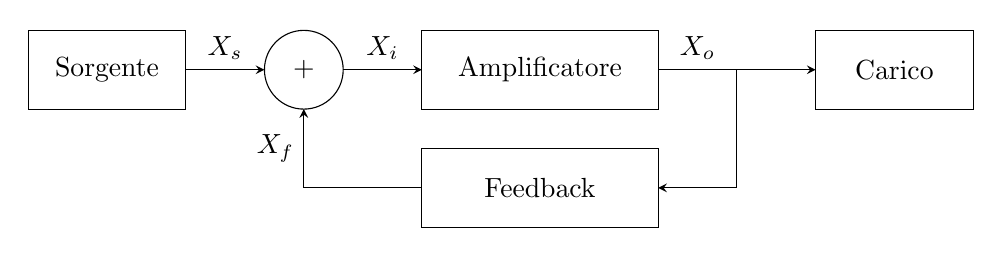
\begin{tikzpicture}
	\node at(0,0){Sorgente};
	\draw(-1,0.5)--(1,0.5)--(1,-.5)--(-1,-.5)--(-1,.5);
	\draw[-stealth](1,0)--(2,0);
	\draw(3,0)arc[start angle=0, end angle=360, x radius=0.5, y radius=0.5];
	\node at(2.5,0){+};
	\draw[-stealth](3,0)--(4,0);
	\node at(5.5,0){Amplificatore};
	\draw(4,.5)--(7,.5)--(7,-.5)--(4,-.5)--(4,.5);
	\node at(5.5,-1.5){Feedback};
	\draw(4,-1)--(7,-1)--(7,-2)--(4,-2)--(4,-1);
	\draw[-stealth](7,0)--(9,0);
	\draw[-stealth](8,0)--(8,-1.5)--(7,-1.5);
	\draw[-stealth](4,-1.5)--(2.5,-1.5)--(2.5,-0.5);
	\node at(10,0){Carico};
	\draw(9,0.5)--(11,.5)--(11,-.5)--(9,-.5)--(9,.5);
	\node at(1.5,0)[above]{$X_s$};
	\node at(3.5,0)[above]{$X_i$};
	\node at(2.5,-1)[left]{$X_f$};
	\node at(7.5,0)[above]{$X_o$};
	\end{tikzpicture}
	\caption{sistema con feedback.}
	\label{fig:feedback}
\end{figure}
Supponiamo che i guadagni dell'amplificatore e della rete di feedback siano rispettivamente $A$ e $\beta$. $A$ è detto open loop gain, dato che coincide con il guadagno in assenza di feedback, mentre $\beta$ è detto feedback gain. Si trova facilmente
\[X_o=AX_i,\qquad\qquad X_f=\beta X_o,\qquad\qquad X_i=X_s+X_f\]
e dunque l'output è
\[X_o=\frac{A}{1-\beta A}X_i\]
$L=\beta A$ è detto loop gain. Inoltre, il guadagno dell'intero sistema è
\[A_f=\frac{A}{1-\beta A}\]
Con la nostra convenzione sui segni, un feedback negativo corrisponde a $\beta<0$.\footnote{In generale è $\beta A\in \C$. Per semplicità supponiamo $\beta$ reale e includiamo tutte le fasi in $A$.} Allora si deduce facilmente che il denominatore in $A_f$ può annullarsi solo se il feedback è positivo. In generale, $L$ dipende dalla frequenza: possiamo passare in trasformata di Fourier e porre\[L=|L(\omega)|e^{j\phi(\omega)}\] Supponiamo ora che il feedback sia positivo, che la sorgente sia assente ($X_s=0$) e che l'input del feedback non sia collegato all'output dell'amplificatore. Se iniettiamo un segnale di test $X_t$ al feedback, allora il segnale in uscita dall'amplificatore è $X_o=LX_t$. Se ora iniettiamo nuovamente questo segnale al feedback per $n$ volte (cioè di fatto chiudiamo la rete di feedback), allora in uscita avremo un segnale
\[X_o^{(n)}=|L(\omega)|^ne^{jn\phi(\omega)}X_t\]
Abbiamo quindi diversi casi
\begin{itemize}
	\item $|L(\omega)|<1$: il segnale in uscita tende a smorzarsi.
	\item $|L(\omega)|>1$: il segnale in uscita diverge in modulo, ma verosimilmente il sistema satura e l'ampiezza raggiunge un massimo finito.
	\item $|L(\omega)=1|$: in tal caso, se $\phi(\omega)=2k\pi$ per qualche $k\in \Z$, ossia se $X_o^{(n)}=X_t$, il segnale è stabile. In realtà, ci aspettiamo un'oscillazione. La condizione $L=1$ è detta condizione di Barkhausen e in questa situazione il guadagno del sistema diverge.
	
	Se invece $\phi$ non è multiplo di $2\pi$ non accade, il sistema viene sfasato ad ogni giro, quindi ci aspettiamo un segnale che media a zero.
\end{itemize}
Tipicamente, il guadagno dell'amplificatore è non lineare, in particolare è più o meno costante rispetto al segnale di ingresso fino a quando questo non raggiunge un valore critico $\overline{X}_i$. Oltre tale valore, il guadagno diminuisce al crescere di $X_i$. Questo significa che partendo da un piccolo segnale in ingresso, prima o poi riusciamo sempre a raggiungere la condizione $|L(\omega)|=1$. Dunque una non linearità nel guadagno migliora la stabilità in ampiezza del segnale. Se ora esiste una certa frequenza per cui $\phi(\omega)=0$, allora solo questa frequenza viene selezionata e amplificata dal circuito, mentre le altre non vengono amplificate. Da un punto di vista sperimentale, vorremmo che la fase $\phi$ dipenda fortemente dalla frequenza, per avere un segnale il più possibile monocromatico.
\subsubsection{Teorema di Miller}
Consideriamo un sistema con feedback come quello in figura \ref{fig:miller1}. Allora per il calcolo delle impedenze di ingresso e di uscita il circuito è equivalente a quello in figura \ref{fig:miller2}, dove
\[Z_1=\frac{Z}{1-k},\qquad\qquad Z_2=\frac{-kZ}{1-k}\]
\begin{figure}[h!]
	\centering
	\begin{circuitikz}
		\draw(0,0)to[short,-o](2.5,0)node[anchor=west]{1};
		\draw(1,0)to[short,*-](1,1)to[generic=$Z$](6,1)to[short, -*](6,0);
		\draw(7,0)to[short,-o](4.5,0)node[anchor=east]{2};
		\draw(0,-1.5)to(7,-1.5);
		\draw(2,0.5)to(5,0.5)to(5,-2)to(2,-2)to(2,.5);
		\draw(3.5,-1.5)to(3.5,-2)node[ground]{};
		\draw(3.5,-0.75)node{$k$};
		
	\end{circuitikz}
	\caption{circuito con feedback del teorema di Miller.}
	\label{fig:miller1}
\end{figure}
\begin{figure}[h!]
	\centering
	\begin{circuitikz}
		\draw(0,0)to[short,-o](2.5,0)node[anchor=west]{1};
		\draw(1,0)to[generic=$Z_1$, *-*](1,-1.5);
		\draw(6,0)to[generic=$Z_2$, *-*](6,-1.5);
		\draw(7,0)to[short,-o](4.5,0)node[anchor=east]{2};
		\draw(0,-1.5)to(7,-1.5);
		\draw(2,0.5)to(5,0.5)to(5,-2)to(2,-2)to(2,.5);
		\draw(3.5,-1.5)to(3.5,-2)node[ground]{};
		\draw(3.5,-0.75)node{$k$};
		
	\end{circuitikz}
	\caption{circuito equivalente del teorema di Miller.}
	\label{fig:miller2}
\end{figure}
Per la dimostrazione, siano $I\ped{in},I\ped{out},I_1,I_2$ e $I_Z$ rispettivamente la corrente di ingresso, la corrente di uscita, la corrente entrante nel polo 1, la corrente uscente dal polo 2 e la corrente in $Z$. Allora è
\[I\ped{in}=I_Z+I_1,\qquad\qquad I\ped{out}=I_Z+I_2\]
Se $V_1$ e $V_2$ sono le tensioni in entrata e in uscita, allora $V_2=kV_1$ e 
\[I_Z=\frac{1-k}{Z}V_1\]
Per concludere basta allora richiedere che nel circuito in figura \ref{fig:miller2}, per una corrente di ingresso $I\ped{in}$ e una tensione di ingresso $V_1$, allora le correnti in $Z_1$ e $Z_2$ sono rispettivamente $I_Z$ e $I_{-Z}$. Ma questo significa imporre
\[I_Z=\frac{V_1}{Z_1}=-\frac{kV_1}{Z_2}\]
ossia
\[Z_1=\frac{Z}{1-k},\qquad\qquad Z_2=-\frac{kZ}{1-k}\]
Applichiamo il teorema per migliorare l'analisi dell'amplificatore di carica. In un rivelatore reale, in genere è presente una capacità parassita $C_D$ in parallelo al generatore di corrente, come in figura \ref{fig:millercaricacond}. 
\begin{figure}[h!]
	\centering
	\begin{circuitikz}
		\draw(0,0)node[op amp]{};
		\draw(-4,-1.5)node[ground]{}to[ioosource=$i(t)$](-4,0.49)to(-1.2,0.49)to(-1.2,1.5)to[C=$C$](2,1.5)to(2,0);
		\draw(-4,-1.5)to(-2,-1.5)to[C=$C_D$](-2,.49);
		\draw(1,0)to(2.5,0)node[anchor=west]{$V\ped{out}$};
		\draw(-1.2,-1.5)node[ground]{}to(-1.2,-0.49);
	\end{circuitikz}
	\caption{amplificatore di carica con capacità parassita.}
	\label{fig:millercaricacond}
\end{figure}

Dunque usando il teorema di Miller, il circuito è equivalente al circuito in figura \ref{fig:millercarica}.
\begin{figure}[h!]
	\centering
	\begin{circuitikz}
		\draw(-3,-1.5)to[ioosource=$i(t)$](-3,0)to[short,-o](2.5,0)node[anchor=west]{1};
		\draw(-1,-1.5)to[C=$C_D$,*-*](-1,0);
		\draw(1,0)to[generic=$Z_1$, *-*](1,-1.5);
		\draw(6,0)to[generic=$Z_2$, *-*](6,-1.5);
		\draw(7,0)to[short,-o](4.5,0)node[anchor=east]{2};
		\draw(-3,-1.5)to(7,-1.5);
		\draw(2,0.5)to(5,0.5)to(5,-2)to(2,-2)to(2,.5);
		\draw(3.5,-1.5)to(3.5,-2)node[ground]{};
		\draw(3.5,-0.75)node{$k$};
		
		
	\end{circuitikz}
	\caption{circuito equivalente all'amplificatore di carica.}
	\label{fig:millercarica}
\end{figure}
dove
\[Z_1=\frac{1}{sC(A_d+1)}\]
L'analisi fatta in precedenza è valida se quasi tutta la carica iniettata si accumula su $Z_1$ e non su $C_D$. Questo significa richiedere che $C_1=C(A_d+1)$ sia molto più grande di $C_D$. Questa condizione è facilmente realizzabile, dato che $A_d\gg1$. Comunque, è bene non scegliere $C$ troppo elevata, dato che il picco del segnale in uscita è $Q/C$, e rischia di diventare troppo basso.

Vediamo ora alcune proprietà di un circuito con feedback negativo.
\subsubsection{Desensibilizzazione del guadagno}
Si noti che
\[\frac{\d A_f}{A_f}=\frac{\d A}{A}\frac{1}{1-\beta A}\]
Il fattore $1-\beta A$ è detto fattore di desensibilizzazione. Solitamente $|\beta A|\gg1$, quindi l'incertezza nel circuito con feedback è sensibilmente minore rispetto all'incertezza nel circuito senza feedback, a patto che l'incertezza su $\beta$ sia sufficientemente piccola. Ad esempio, consideriamo l'amplificatore non invertente in figura \ref{fig:opampnoninvert}. La rete di feedback è costituita da $R_1$ e $R_2$ e il feedback gain è
\[\beta=-\frac{1}{1+R_2/R_1}\]
e, se ad esempio $\Delta A/A\simeq50\%$, allora inserendo i valori tipici di $A$ e $\beta$ si trova $\Delta A_f/A_f\simeq0.05\%$.
\subsubsection{Aumento della larghezza di banda}
Supponiamo di avere un amplificatore con un singolo polo, ossia con un guadagno della forma
\[A=\frac{A_M}{1+s/\omega_H}\]
dove $A_M$ è il guadagno di centro banda, ossia a basse frequenze nel nostro modello, e $\omega_H$ è la frequenza di taglio. Allora in presenza di feedback si trova
\[A_f=\frac{A_{Mf}}{1+s/\omega_{Hf}}\]
dove
\[A_{Mf}=\frac{A_M}{1-\beta A_M},\qquad\qquad\omega_{Hf}=\omega_H(1-\beta A_M)\]
dunque se il feedback è negativo la banda passante aumenta, in genere di molto dato che spesso è $|\beta A_M|\gg1$. Si noti che il $GBW$ non varia aggiungendo il feedback, in altre parole la banda passante aumenta a discapito del guadagno massimo. Questo è un fatto molto ricorrente: il feedback introduce diversi vantaggi a discapito del guadagno massimo del sistema.
\subsubsection{Miglioramento delle impedenze di ingresso e di uscita}
In maniera informale, il feedback migliora le impedenze di ingresso e di uscita del sistema. Per essere più quantitativi, dobbiamo distinguere tra quattro tipi diversi di amplificatore, a seconda che in ingresso e in uscita si considerino correnti o tensioni. Nei diversi casi varia il modo in cui si fa sampling e summing, ossia il modo in cui si preleva il segnale all'uscita e lo si introduce di nuovo all'ingresso.
\paragraph{Amplificatore di tensione}
In tal caso sia in ingresso che in uscita abbiamo delle tensoni. Lo schema circuitale è quindi quello di figura \ref{fig:amplivv}. Qui il sampling è in parallelo, il summing in serie.
\begin{figure}[h!]
	\centering
	\begin{circuitikz}
		\draw(2,-5.5)node[anchor=west]{$+$}to(0,-5.5)to[sV=$V_S$](0,0)to[R=$R_S$](2,0)node[anchor=west]{$+$};
		\draw(2,0.5)to(5,.5)to(5,-2.5)to(2,-2.5)to(2,.5);
		\draw(2,-3)to(5,-3)to(5,-6)to(2,-6)to(2,-3);
		\draw(2,-2)node[anchor=west]{$-$}to(1.5,-2)to(1.5,-3.5)to(2,-3.5)node[anchor=west]{$-$};
		\draw(3.5,-1)node{$A_V$};
		\draw(3.5,-4.5)node{$\beta$};
		\draw(5,0)node[anchor=east]{$+$}to(6.5,0)to[R=$R_L$](6.5,-2)to(5,-2)node[anchor=east]{$-$};
		\draw(5.5,0)to[short,*-](5.5,-1.9);
		\draw(5.5,-2.1)to(5.5,-3.5)to(5,-3.5);
		\draw(6.5,-2)to[short,*-](6.5,-5.5)to(5,-5.5);
	\end{circuitikz}
	\caption{amplificatore di tensione con feedback.}
	\label{fig:amplivv}
\end{figure}
Idealmente, per un circuito del genere vorremmo una resistenza di ingresso infinita e una resistenza di uscita nulla. Se l'amplificatore ha una resistenza di ingresso $R\ped{in}$ e una resistenza di uscita $R\ped{out}$, il circuito è quello mostrato in figura \ref{fig:amplivvimp}.
\begin{figure}[h!]
	\centering
	\begin{circuitikz}
		\draw(2,-5.5)to(0,-5.5)to[sV=$V_S$](0,0)to[R=$R_S$](2,0);
		\draw(2,0.5)to(5,.5)to(5,-2.5)to(2,-2.5)to(2,.5);
		\draw(2,-3)to(5,-3)to(5,-6)to(2,-6)to(2,-3);
		\draw(2,-2)to(1.5,-2)to(1.5,-3.5)to(2,-3.5);
		\draw(5,0)to(6.5,0)to[R=$R_L$](6.5,-2)to(5,-2);
		\draw(5.5,0)to[short,*-](5.5,-1.9);
		\draw(5.5,-2.1)to(5.5,-3.5)to(5,-3.5);
		\draw(6.5,-2)to[short,*-](6.5,-5.5)to(5,-5.5);
		\draw(2,0)to(2.4,0)to[R, l_=$R\ped{in}$](2.4,-2)to(2,-2);
		\draw(5,-2)to(3.1,-2)to[sV, l_=$A_VV\ped{in}$](3.1,0)to[R, l_=$R\ped{out}$](5,0);
		\draw(2,-3.5)to(2.5,-3.5)to[sV=$\beta V\ped{out}$](2.5,-5.5)to(2,-5.5);
		\draw[-latex](1.8,1)node[anchor=south]{$V\ped{in}$}to(1.8,0.2);
		\draw[-latex](7.5,-1)to(7.5,-2);
		\draw[-latex](7.5,-1)node[anchor=west]{$V\ped{out}$}to(7.5,0);
	\end{circuitikz}
	\caption{amplificatore di tensione con feedback e resistenze di ingresso e uscita.}
	\label{fig:amplivvimp}
\end{figure}
Usualmente, la resistenza della sorgente è trascurabile, mentre il carico è molto grande. Lavorando in queste approssimazioni, si trovano le resistenze di ingresso e di uscita
\begin{align*}
	R\ped{in}^f&=\frac{V_S}{V\ped{in}/R\ped{in}}=R\ped{in}(1-\beta A_V)>R\ped{in}\\
	R\ped{out}^f&=\frac{A_fV_s}{A_VV_s/R\ped{out}}=\frac{R\ped{out}}{1-\beta A_V}<R\ped{out}
\end{align*}
Dunque il feedback porta il sistema più vicino all'idealità. Questo è vero anche con gli altri tipi di amplificatore, in particolare per le resistenze di ingresso e di uscita si trova
\begin{table}[h!]
	\centering
	\begin{tabular}{|c| c| c| c|}
		\hline Summing&$R\ped{in}^f$&Sampling&$R\ped{out}^f$\\\hline
		serie&$R\ped{in}(1-\beta A_V)$&parallelo&$\dfrac{R\ped{out}}{1-\beta A_V}$\\
		parallelo&$\dfrac{R\ped{in}}{1-\beta A_V}$&serie&$R\ped{out}(1-\beta A_V)$\\\hline
	\end{tabular}
\end{table}
e, come vedremo, questi risultati si avvicinano maggiormente alle condizioni di idealità.
\paragraph{Transconduttanza} In tal caso in ingresso c'è una tensione (cioè summing in serie) e in uscita una corrente (cioè sampling in serie). Il circuito è riportato in figura \ref{fig:amplivi}. Idealmente, le resistenze di ingresso e di uscita dovrebbero essere infinite. Si noti che il prodotto $\beta G_M$ deve essere sempre adimensionale, ma le dimensioni dei singoli fattori variano da amplificatore ad amplificatore: qui $G_M$ ha le dimensioni di una conduttanza e $\beta$ le dimensioni di una resistenza.
\begin{figure}[h!]
	\centering
	\begin{circuitikz}
		\draw(2,-5.5)node[anchor=west]{$+$}to(0,-5.5)to[sV=$V_S$](0,0)to[R=$R_S$](2,0)node[anchor=west]{$+$};
		\draw(2,0.5)to(5,.5)to(5,-2.5)to(2,-2.5)to(2,.5);
		\draw(2,-3)to(5,-3)to(5,-6)to(2,-6)to(2,-3);
		\draw(2,-2)node[anchor=west]{$-$}to(1.5,-2)to(1.5,-3.5)to(2,-3.5)node[anchor=west]{$-$};
		\draw(3.5,-1)node{$G_M$};
		\draw(3.5,-4.5)node{$\beta$};
		\draw(5,0)to(6,0)to[R=$R_L$](6,-5.5)to(5,-5.5);
		\draw(5,-2)to(5.5,-2)to(5.5,-3.5)to(5,-3.5);
	\end{circuitikz}
	\caption{transconduttanza con feedback.}
	\label{fig:amplivi}
\end{figure}
\paragraph{Amplificatore di corrente}Sia in ingresso che in uscita abbiamo delle correnti, quindi abbiamo un sampling in serie e un summing in parallelo. Il circuito è in figura \ref{fig:ampliii}. Idealmente vorremo una resistenza di ingresso nulla e una resistenza di uscita infinita.
\begin{figure}[h!]
	\centering
	\begin{circuitikz}
		\draw(2,-2)to(-2,-2)to[ioosource=$i_S$](-2,0)to(2,0);
		\draw(0,-2)to[R=$R_S$](0,0);
		\draw(2,0.5)to(5,.5)to(5,-2.5)to(2,-2.5)to(2,.5);
		\draw(2,-3)to(5,-3)to(5,-6)to(2,-6)to(2,-3);
		\draw(2,-2)to[short, -*](1.5,-2)to(1.5,-3.5)to(2,-3.5);
		\draw(3.5,-1)node{$A_I$};
		\draw(3.5,-4.5)node{$\beta$};
		\draw(5,0)to(6,0)to[R=$R_L$](6,-5.5)to(5,-5.5);
		\draw(5,-2)to(5.5,-2)to(5.5,-3.5)to(5,-3.5);		\draw(0.5,0)to[short,*-](0.5,-1.9);
		\draw(0.5,-2.1)to(0.5,-5.5)to(2,-5.5);
	\end{circuitikz}
	\caption{amplificatore di corrente con feedback.}
	\label{fig:ampliii}
\end{figure}
\paragraph{Transresistenza}
Infine, se in ingresso abbiamo una corrente e in uscita una tensione, si parla di transresistenza. Sia il sampling che il summing sono in parallelo. Il circuito è riportato in figura \ref{fig:ampliiv}. $R_M$ ha le dimensioni di una resistenza, $\beta$ le dimensioni di una conduttanza. Idealmente vorremmo resistenze di ingresso e di uscita nulle.
\begin{figure}[h!]
	\centering
	\begin{circuitikz}
		\draw(2,-2)to(-2,-2)to[ioosource=$i_S$](-2,0)to(2,0);
		\draw(0,-2)to[R=$R_S$](0,0);
		\draw(2,0.5)to(5,.5)to(5,-2.5)to(2,-2.5)to(2,.5);
		\draw(2,-3)to(5,-3)to(5,-6)to(2,-6)to(2,-3);
		\draw(2,-2)to[short, -*](1.5,-2)to(1.5,-3.5)to(2,-3.5);
		\draw(3.5,-1)node{$A_I$};
		\draw(3.5,-4.5)node{$\beta$};
		\draw(0.5,0)to[short,*-](0.5,-1.9);
		\draw(0.5,-2.1)to(0.5,-5.5)to(2,-5.5);
			\draw(5,0)node[anchor=east]{$+$}to(6.5,0)to[R=$R_L$](6.5,-2)to(5,-2)node[anchor=east]{$-$};
		\draw(5.5,0)to[short,*-](5.5,-1.9);
		\draw(5.5,-2.1)to(5.5,-3.5)to(5,-3.5)node[anchor=east]{$+$};
		\draw(6.5,-2)to[short,*-](6.5,-5.5)to(5,-5.5)node[anchor=east]{$-$};
	\end{circuitikz}
	\caption{transresistenza con feedback.}
	\label{fig:ampliiv}
\end{figure}
\subsection{Applicazione dell'OpAmp: oscillatori a feedback positivo}
In questa sezione vediamo degli oscillatori, ossia dei circuiti in cui non è presente un input, e alla cui uscita si ha un segnale oscillante. Riprendiamo i risultati della sezione precedente: per avere oscillazioni deve essere soddisfatta la condizione di Barkhausen
\[A\beta=1\]
che, all'atto pratico, è di difficile realizzazione. Supponiamo, al solito, che sia $A$ reale e $\beta$ complesso. Si introducono quindi delle non linearità in $A$ per avere $|A\beta|=1$, poi $\beta$ seleziona solo le frequenze per cui effettivamente $A\beta=1$. Per avere stabilità in frequenza e in ampiezza si richiede poi che le derivate della fase e del modulo di $A\beta$, valutate in $A\beta=1$, siano grandi, in modo da avere un segnale pulito. In queste condizioni, all'uscita dovremmo avere un'oscillazione sinusoidale, ma realisticamente ci saranno delle distorsioni, a causa della tendenza alla saturazione. Supponiamo ora che l'amplificare sia invertente, ossia $A<0$. Allora è chiaro che la fase data dal circuito di feedback deve essere $\pi$. Consideriamo una generica funzione di risposta in trasformata di Laplace
\[\tilde{G}(s)=\frac{P(s)}{Q(s)}\]
dove $P$ e $Q$ sono polinomi a coefficienti reali. Supponiamo inoltre, per semplicità, che $P$ e $Q$ abbiano solo zeri reali. Allora la fase $\phi(\omega)$ del circuito di feedback è data da
\[e^{j\phi(\omega)}=\frac{\tilde{G}(j\omega)}{|\tilde{G}(j\omega)|}\]
Cioè $\phi$ identifica in $\S^2$ il versore a secondo membro. Chiaramente, ogni zero $\tilde{s}$ di $P$ (contato con molteplicità) contribuisce a $\phi(\omega)$ con il termine $\pi-\arctan(\omega/\tilde{s})$, mentre ogni zero $\tilde{s}'$ di $Q$ (di nuovo, contato con molteplicità) contribuisce con un termine $-\pi+\arctan(\omega/\tilde{s}')$ allo sfasamento. Questo significa che la differenza tra lo sfasamento a basse frequenze e lo sfasamento ad alte frequenze è
\[\lim\limits_{\Omega\to+\infty}\phi(\Omega)-\lim\limits_{\omega\to0}\phi(\omega)=\frac{\pi}{2}\left(\deg P-\deg Q\right)\]
Consideriamo ora il filtro più semplice possibile, ossia un filtro $RC$: è chiaro da quanto visto nella sezione sui filtri che un solo circuito di sfasamento non è sufficiente per raggiungere $\phi=\pm\pi$. In linea di principio, sarebbero sufficienti due passa-alto in serie per avere l'obiettivo desiderato nel limite $\omega\to+\infty$: questa disposizione non è però la migliore, dato che lo sfasamento non è mai esattamente $\pi$, e inoltre la derivata della fase tende a zero quando $\omega\to+\infty$, quindi non avremmo stabilità in frequenza. La scelta migliore è lavorare con almeno tre circuiti di sfasamento, ossia consideriamo il circuito in figura \ref{fig:oscsfas}.
\begin{figure}[h!]
	\centering
	\begin{circuitikz}
		\draw(0,0)to(2,0)to(2,-2)to(0,-2)to(0,0);
		\draw(1,-1)node{$-A$};
		\draw(0,-1)to(-.5,-1)to(-.5,1)to(9,1)to(9,-1)to[short, -*](8,-1)to[generic, l_=$Z_1$, -*](6,-1)to[generic, l_=$Z_1$, -*](4,-1)to[generic, l_=$Z_1$](2,-1);
		\draw(4,-1)to[generic=$Z_2$](4,-3)to(8,-3)to[generic, l_=$Z_2$](8,-1);
		\draw(6,-1)to[generic=$Z_2$, -*](6,-3)node[ground]{};
		\draw(2.2,-1)node[anchor=south]{$V_4$};
		\draw(4,-1)node[anchor=south]{$V_3$};
		\draw(6,-1)node[anchor=south]{$V_2$};
		\draw(8,-1)node[anchor=south]{$V_1$};
		\draw[-latex](3.7,-1.7)to(3.7,-2)node[anchor=east]{$i_3$}to(3.7,-2.3);
		\draw[-latex](5.7,-1.7)to(5.7,-2)node[anchor=east]{$i_2$}to(5.7,-2.3);
		\draw[-latex](7.7,-1.7)to(7.7,-2)node[anchor=east]{$i_1$}to(7.7,-2.3);		
		\draw[-latex](8.5,1.2)to(8,1.2)node[anchor=south]{$i$}to(7.5,1.2);
	\end{circuitikz}
	\caption{oscillatore a sfasamento.}
	\label{fig:oscsfas}
\end{figure}

\noindent Supponiamo inoltre che la corrente entrante da sinistra nell'amplificatore sia nulla, ossia $i=0$. Allora si ottiene
\begin{align*}
	V_2&=V_1+Z_1i_1\\
	V_3&=V_2+Z_1(i_1+i_2)\\
	V_4&=V_3+Z_1(i_1+i_2+i_3)	
\end{align*}
Dunque, posto $y=Z_1/Z_2$ è
\begin{align*}
	i_1&=\frac{V_1}{Z_2}\\i_2&=i_1(1+y)\\
	i_3&=i_1(1+2y+y(1+y))\\
\end{align*}
e in definitiva la condizione di Barkhausen è
\[-A=1+6y+5y^2+y^3\]
Se ora prendiamo come circuito di sfasamento un filtro passa-alto $RC$, ossia $Z_1=1/(j\omega C)$ e $Z_2=R$, si trovano le due equazioni
\[\begin{cases}
6y+y^3=0\\1+5y^2=-A	
\end{cases}\]
che hanno per soluzioni $y=\pm j\sqrt{6}$ e $A=29$. Il circuito oscilla quindi alla frequenza $\omega=1/(\sqrt{6}RC)$. Per l'implementazione in un circuito reale, si può pensare di utilizzare un OpAmp e di costruire il circuito in figura \ref{fig:opamposcillamale}.
\begin{figure}[h!]
	\centering
	\begin{circuitikz}
		\draw(0.8,-1)node[op amp]{};
		\draw(-.4,-.51)to[R=$R_1$](-2.4,-.51)to(-2.4,2)to(9,2)to(9,-1)to[short, -*](8,-1)to[C, l_=$C$, -*](6,-1)to[C, l_=$C$, -*](4,-1)to[C, l_=$C$](2,-1);
		\draw(4,-1)to[R=$R$](4,-3)to(8,-3)to[R, l_=$R$](8,-1);
		\draw(6,-1)to[R=$R$, -*](6,-3)node[ground]{};
		\draw(-.5,-.51)to(-.5,.51)to[R=$R_2$](2,.51)to(2,-1);
		\draw(-.4,-1.49)to(-.4,-2)node[ground]{};
	\end{circuitikz}
	\caption{oscillatore a sfasamento non funzionante.}
	\label{fig:opamposcillamale}
\end{figure}
Questo circuito non può funzionare, o meglio la nostra analisi non si applica a questo circuito. In particolare, l'assuzione $i=0$ non è vera in generale. Una possibile soluzione è l'aggiunta di un follower, come in figura \ref{fig:opamposcillafollower}, ma la presenza di due OpAmp la rende difficilmente realizzabile su larga scala a costi ragionevoli.
\begin{figure}[h!]
	\centering
	\begin{circuitikz}
		\draw(0.8,-1)node[op amp]{};
		\draw(-.4,-.51)to[R=$R_1$](-2.4,-.51)to(-2.4,2)to(2.3,2)to(2.3,3.5)to(5,3.5)to(5,2)to(4.5,2);
		\draw(2.3,1.51)to(2.3,0.8)to(9,0.8)to(9,-1)to[short, -*](8,-1)to[C, l_=$C$, -*](6,-1)to[C, l_=$C$, -*](4,-1)to[C, l_=$C$](2,-1);
		\draw(4,-1)to[R=$R$](4,-3)to(8,-3)to[R, l_=$R$](8,-1);
		\draw(6,-1)to[R=$R$, -*](6,-3)node[ground]{};
		\draw(-.5,-.51)to(-.5,.51)to[R=$R_2$](2,.51)to(2,-1);
		\draw(-.4,-1.49)to(-.4,-2)node[ground]{};
		\draw(3.5,2)node[op amp]{};
	\end{circuitikz}
	\caption{oscillatore a sfasamento con follower.}
	\label{fig:opamposcillafollower}
\end{figure}
Alternativamente, possiamo forzare l'entrata negativa dell'OpAmp a essere a massa, modificando il circuito come in figura \ref{fig:opamposcilla}.
\begin{figure}[h!]
	\centering
	\begin{circuitikz}
		\draw(0.8,-1)node[op amp]{};
		\draw(-.4,-.51)to(-1,-.51)to(-1,2)to(8,2)to[R=$R$](8,-1)to[C, l_=$C$, -*](6,-1)to[C, l_=$C$, -*](4,-1)to[C, l_=$C$](2,-1);
		\draw(4,-1)to[R=$R$](4,-3)to(5,-3)node[ground]{}to(6,-3)to[R, l_=$R$](6,-1);
		\draw(-.5,-.51)to(-.5,.51)to[R=$R_F$](2,.51)to(2,-1);
		\draw(-.4,-1.49)to(-.4,-2)node[ground]{};
	\end{circuitikz}
	\caption{oscillatore a sfasamento quasi funzionante.}
	\label{fig:opamposcilla}
\end{figure}
Anche con questa disposizione, avere un guadagno esattamente pari a 29 è molto difficile. Si può introdurre una non linearità controllata che permetta di selezionare il guadagno corretto. Questo risultato si ottiene sostituendo $R_F$ come in figura \ref{fig:opamposcillabene}, con la condizione aggiuntiva
\[\frac{R_1}{R}<29<\frac{R_1+R_2}{R}\]
\begin{figure}[h!]
	\centering
	\begin{circuitikz}
		\draw(0.8,-1)node[op amp]{};
		\draw(-.4,-.51)to(-3,-.51)to(-3,5)to(8,5)to[R=$R$](8,-1)to[C, l_=$C$, -*](6,-1)to[C, l_=$C$, -*](4,-1)to[C, l_=$C$](2,-1);
		\draw(4,-1)to[R=$R$](4,-3)to(5,-3)node[ground]{}to(6,-3)to[R, l_=$R$](6,-1);
		\draw(-2.5,-.51)to(-2.5,1.51)to[R=$R_1$](-.5,1.51)to[R=$R_2$](1.5,1.51)to(2,1.51)to(2,-1);
		\draw(-.4,-1.49)to(-.4,-2)node[ground]{};
		\draw(-.5,.51)to(-.5,2.51)to[diode](1.5,2.51)to(1.5,.51)to[diode](-.5,.51);
	\end{circuitikz}
	\caption{oscillatore a sfasamento quasi funzionante.}
	\label{fig:opamposcillabene}
\end{figure}

Un altro tipo di oscillatore è l'oscillatore a ponte di Wien. In questo oscillatore abbiamo sia un passa-alto che un passa-basso nel circuito di sfasamento. Lo schema di base del circuito è quello in figura \ref{fig:wien}, dove non stiamo supponendo che l'amplificatore sia invertente.
\begin{figure}[h!]
	\centering
	\begin{circuitikz}
		\draw(0,0)to(2,0)to(2,-2)to(0,-2)to(0,0);
		\draw(1,-1)node{$A$};
		\draw[-latex](5,1.2)to(4.5,1.2)node[anchor=south]{$i$}to(4,1.2);
		\draw(0,-1)to(-0.5,-1)to(-0.5,1)to(6,1)to(6,-1)to[short, *-*](6,-1.5)to(7,-1.5)to[C=$C$](7,-3.5)to(6,-3.5)node[ground]{};
		\draw(6,-1.5)to(5,-1.5)to[R=$R$](5,-3.5)to(6,-3.5);
		\draw(2,-1)to[R=$R$](4,-1)to[C=$C$](6,-1);
	\end{circuitikz}
	\caption{oscillatore a ponte di Wien.}
	\label{fig:wien}
\end{figure}
Anche qui lavoriamo nell'ipotesi $i=0$. Allora, posto $\omega_0=1/(RC)$ e
\[Z_S=R\left(1+\frac{\omega_0}{s}\right),\qquad\qquad Z_P=\frac{R}{1+s/\omega_0}\]
un semplice calcolo dà
\[\beta=\frac{Z_P}{Z_S+Z_P}=\frac{s\omega_0}{s^2+3\omega_0s+\omega_0^2}\]
e ha uno zero e due poli. La condizione di Barkhausen è
\[A=1+\frac{Z_S}{Z_P}\]
Per $s$ immaginario pure si trova, prendendo la parte reale e la parte immaginaria,
\[\begin{cases}
A=3\\\dfrac{\omega_0}{s}+\dfrac{s}{\omega_0}=0
\end{cases}\]
quindi per avere oscillazioni deve essere $A=3$, ossia l'amplificatore è non invertente. La frequenza delle oscillazioni è $\omega_0$. Il circuito associato è riportato in figura \ref{fig:pontewien}.
\begin{figure}[h!]
	\centering
	\begin{circuitikz}
		\draw(1,0)node[op amp]{};
		\draw(-3.2,1.5)node[ground]{}to[R=$R$](-1.2,1.5)to[pR=$R$, mirror](0.8,1.5)to[R=$R$](2.8,1.5)to[R, l_=$R$](4.8,1.5)to(4.8,0)to[C=$C$](4.8,-2)to[R=$R$](4.8,-4)to(5.8,-4)to[C=$C$](5.8,-6)to(4.8,-6)node[ground]{}to(3.8,-6)to[R=$R$](3.8,-4);
		\draw(-.2,-.49)to(-.2,-4)to[short, -o](6,-4)node[anchor=west]{$V\ped{out}$};
		\draw(-.2,.49)to(-.2,1.2);
		\draw(2.2,0)to[short,-*](4.8,0);
		\draw(2.8,1.5)to[short, *-*](2.8,2.5);
		\draw(4.8, 1.5)to[short, *-*](4.8,2.5);
		\draw(4.8,2.5)to[diode](2.8,2.5)to(2.8,3.5)to[diode](4.8,3.5)to(4.8,2.5);
	\end{circuitikz}
	\caption{oscillatore a ponte di Wien.}
	\label{fig:pontewien}
\end{figure}
\subsection{Stabilità e funzione di risposta}
Vediamo, come ultima cosa, la stabilità di un sistema. Ricordiamo che
\[\mathcal{L}[e^{s_0t}](s)=\frac{1}{s-s_0}\]
dunque la parte immaginaria di $s_0$ è la frequenza di oscillazione, mentre la parte reale di $s_0$ è l'inverso della costante di tempo: se $\Re s_0>0$, l'ampiezza del segnale diverge, mentre se $\Re s_0<0$, l'ampiezza del segnale si smorza. Se invece $\Re s_0=0$, allora abbiamo delle vere e proprie oscillazioni periodiche. Come polinomio di secondo grado tipico consideriamo il polinomio
\[P_2(s)=s^2+\frac{\omega_0}{Q}s+\omega_0^2\]
$\omega_0$ è la (pseudo-)frequenza di oscillazione e $Q$ è detto $Q$-valore. Ci sono molti sistemi fisici in cui compare questo polinomio. Ad esempio, nell'oscillatore a ponte di Wien si ha 
\[\tilde{G}(s)=\frac{A}{1-\beta A}=A\frac{s^2+3\omega_0s+\omega_0^2}{s^2+(3-A)\omega_0s+\omega_0^2}\]
e dunque $Q^{-1}=3-A$. Un altro esempio è un circuito $RLC$ come quello di figura \ref{fig:rlc}: la funzione di trasferimento è
\[\tilde{G}(s)=\frac{1}{LC}\frac{1}{s^2+\dfrac{s}{CR}+\dfrac{1}{LC}}\]
ossia $\omega_0^2=1/(LC)$ e $Q=R\sqrt{C/L}$.
\begin{figure}[h!]
	\centering
	\begin{circuitikz}
		\draw(0,0)node[anchor=east]{$V\ped{in}$}to[short, o-](1,0)to[L=$L$](2.5,0)to[short, -o](6,0)node[anchor=west]{$V\ped{out}$};
		\draw(5,0)to[R=$R$](5,-2);
		\draw(3.5,0)to[C=$C$](3.5,-2)node[ground]{};
		\draw(0,-2)to[short, o-o](6,-2);
	\end{circuitikz}
	\caption{circuito $RLC$.}
	\label{fig:rlc}
\end{figure}

Allo stesso modo, per una particella di massa $m$ legata a una molla di costante elastica $k$ e soggetta ad attrito viscoso $-\beta\dot{x}$, è
\[\tilde{G}(s)=\frac{1}{m}\frac{1}{s^2+\dfrac{\beta}{m}s+\dfrac{k}{m}}\]
e dunque $\omega_0^2=k/m$ e $Q=\sqrt{km}/\beta$. 

Studiamo in dettaglio le radici di $P_2$. Chiaramente
\[s_{1,2}=-\frac{\omega_0}{2Q}\left(1\pm\sqrt{1-4Q^2}\right)\]
quindi
\begin{itemize}
	\item per $Q>1/2$ abbiamo due radici complesse, distinte e con parte reale negativa. Il sistema compie delle oscillazioni smorzate;
	\item per $0<Q<1/2$ abbiamo due radici reali, distinte e negative. Il sistema non oscilla e si smorza;
	\item per $-1/2<Q<0$ abbiamo due radici reali, distinte e positive. Il sistema non oscilla e diverge;
	\item per $Q<-1/2$ abbiamo due radici complesse, distinte e con parte reale positiva. Il sistema compie delle oscillazioni divergenti.
\end{itemize}
Il sistema è quindi stabile solo per $Q>0$. In particolare, per $Q\to+\infty$ si ha $s_{1,2}\to\pm j\omega_0$, dunque si hanno oscillazioni vere e proprie solo quando il termine lineare in $P_2$ è nullo: come sappiamo, il $Q$-valore è legato al rate con cui l'attrito viscoso dissipa energia. Si noti ora che per $|Q|>1/2$ si ha $|s_{1}|=|s_2|=\omega_0$, dato che deve essere $s_1=s_2^*$ e $s_1s_2=\omega_0^2$. Questo significa che le due radici possono sempre essere identificate come due punti della circonferenza del piano complesso $|s|=\omega_0$. Viceversa, per $|Q|<1/2$ le due radici si trovano sull'asse reale e sono una l'inversa circolare dell'altra rispetto alla circonferenza $|s|=\omega_0$.
\newpage
\section{Elettronica digitale}
L'idea base dell'elettronica digitale è la trasformazione di un segnale continuo in un segnale che può avere solo due valori, tipicamente 0 e 1. Per farlo bisogna prima concordare a quali valori della grandezza continua è associato lo 0 e a quali l'1, e questa libertà può portare a implementazioni fisiche diverse di uno stesso circuito logico.
\subsection{Logica booleana}
Sia $\B=\left\{0,1\right\}$. Si dice che $\B$ è l'insieme delle variabili booleane. L'insieme $\B^n$ per $n\in\N$ è l'insieme delle $n$-uple di variabili booleane: spesso si identifica una tale $n$-upla con una stringa di 0 e 1, ossia si fa l'associazione $(X_1,\dots, X_n)\leftrightarrow X_1\dots X_n$.

Una funzione logica booleana è una mappa $b\colon\B^n\to\B$, per un qualche intero non negativo $n$. Possiamo interpretare la funzione come una macchina a $n$ ingressi $X_1\dots X_n$ e un'unica uscita $Y=b(X_1\dots X_n)$. Dato che $\B$ ha cardinalità finita, possiamo costruire una tabella che contenga tutti i valori possibili in ingresso e il valore associato in uscita. Una tale tabella è detta tabella di verità, ma è chiaro che al cresce di $n$ diventa scomodo utilizzare queste tabelle. In questo caso abbiamo supposto che lo stato in uscita non dipendesse dallo stato precedente di $Y$: abbiamo cioè considerato il caso della logica combinatoria. Possiamo anche trattare la logica sequenziale, in cui abbiamo una mappa ${b}\colon\B\times\B^n\to\B$ tale che $Y={b}(Y_0,X_1\dots X_n)$. In questo caso, interpretiamo il primo $\B$ come insieme degli stati in uscita, e dunque l'uscita a un dato istante dipende dallo stato nell'istante precedente. Ancora più in generale, l'uscita può dipende non solo dallo stato immediatamente precedente, ma anche da quelli ancora precedenti. Quindi a funzione logica più generale in logica sequenziale è una mappa $b\colon\mathcal{S}\times\B^n\to \B$, dove $\mathcal{S}$ è lo spazio degli stati della macchina.
\subsection{Logica combinatoria}
Trattiamo per prima la logica combinatoria. \`{E} chiaro che, fissato $n$, il numero di funzioni logiche $b\colon\B^n\to\B$ è
$2^{2^n}$. Questo numero diventa rapidamente intrattabile al crescere di $n$, ma per i primi casi si può fare tutto esplicitamente. Per $n=1$ abbiamo quattro funzioni logiche, le cui tabelle di verità sono riportate nella tabella \ref{tab:ver1}, dove l'ultima riga riportata le notazioni usate per identificare le varie funzioni.
\begin{table}[h!]
	\centering
	\begin{tabular}{c | c c c c}
		$X$&$F_0(X)$&$F_1(X)$&$F_2(X)$&$F_3(X)$\\\hline
		0&0&0&1&1\\1&0&1&0&1\\\hline&0&$X$&$\overline{X}$&1
	\end{tabular}
	\caption{tabelle di verità per funzioni logiche a una variabile.}
	\label{tab:ver1}
\end{table}
$F_0$ e $F_3$ sono banalmente le funzioni identicamente 0 o identicamente 1. $F_1$ è l'identità, mentre $F_2$ è detta \textsf{NOT}. Per questa funzione si usano anche le notazioni $\overline{X}$, $\neg X$, $\sim$$X$ e $!X$.

Le funzioni a due variabili sono 16. Le funzioni di base sono \sf{AND} e \sf{OR}. Per la prima si usano le notazioni $A$\sf{AND}$B$, $A\cdot B$, $A\land B$, $A$\&$B$, e vale 1 se sia $A$ che $B$ sono 1, 0 altrimenti. Per \sf{NOT} si usano le notazioni $A$\sf{NOT}$B$, $A+B$, $A\lor B$, $A|B$, e vale 1 se almeno una tra $A$ e $B$ sono 1, 0 altrimenti. Le funzioni logiche a due variabili sono riportate nella tabella \ref{tab:ver2}.
\begin{table}[h!]
	\begin{tabular}{c  c| c c c c c c c c c c c c c c}
		$A$&$B$&1&2&3&4&5&6&7&8&9&0&11&12&13&14\\\hline
		0&0&1&0&1&0&1&0&1&0&1&0&1&0&1&0\\0&1&0&1&1&0&0&1&1&0&0&1&1&0&0&1\\1&0&0&0&0&1&1&1&1&0&0&0&0&1&1&1\\1&1&0&0&0&0&0&0&0&1&1&1&1&1&1&1\\\hline
		&&$\overline{A+B}$&$\overline{A}\cdot B$&$\overline{A}$&$A\cdot\overline{B}$&$\overline{B}$&$A\oplus B$&$\overline{A\cdot B}$&$A\cdot B$&$A\odot B$&$B$&$\overline{A}+B$&$A$&$A+\overline{B}$&$A+B$\\
	\end{tabular}
	\caption{tabelle di verità per funzioni logiche a una variabile. Sono state omesse le funzioni identicamente 0 o 1.}
	\label{tab:ver2}
\end{table}
$A\oplus B$ è detto \sf{XOR} e vale 1 se esattamente una tra $A$ e $B$ è 1, 0 altrimenti. $A\odot B$ è detta \sf{XNOR} ed è la negazione di \sf{XOR}. Similmente, le negazioni di \sf{AND} e \sf{OR} sono dette rispettivamente \sf{NAND} e \sf{NOR}, ma non hanno simboli specifici. Storicamente, la prima porta ad essere stata implementata è stata proprio \sf{NAND} e l'implementazione è stata fatta tramite transistor.
\subsubsection{Porte logiche}
Una porta logica è un circuito che implementa una funzione logica. I simboli circuitali per le porte logiche a un ingresso sono riportati in figura \ref{fig:porte1}. I simboli circuitali per alcune porte a due ingressi sono invece riportati in figura \ref{fig:porte2}. Come regola generale, la presenza di un pallino prima o dopo la porta indica la negazione della porta stessa.
\begin{figure}[h!]
	\centering
	\begin{circuitikz}
		\draw(0,0)node[buffer]{};
		\draw(3,0)node[not port]{};
	\end{circuitikz}
	\caption{identità (sinistra) e \sf{NOT} (destra).}
	\label{fig:porte1}
\end{figure}
\begin{figure}[h!]
	\centering
	\begin{circuitikz}
		\draw(0,0)node[and port]{};
		\draw(3,0)node[or port]{};
		\draw(6,0)node[nand port]{};
		\draw(9,0)node[nor port]{};
		\draw(12,0)node[xor port]{};
	\end{circuitikz}
	\caption{da sinistra a destra, \sf{AND}, \sf{OR}, \sf{NAND}, \sf{NOR}, \sf{XOR}.}
	\label{fig:porte2}
\end{figure}
\subsubsection{Proprietà delle operazioni booleane}
Le operazioni \sf{AND} e \sf{OR} godono di molteplici proprietà: vediamole nel dettaglio. Per le dimostrazioni, è sufficiente costruire le tabelle di verità dei due membri di tutte le uguaglianze successive.
\begin{itemize}
	\item Associatività
	\begin{align*}
		(A+B)+C&=A+(B+C)\\
		(A\cdot B)\cdot C&=A\cdot(B\cdot C)
	\end{align*}
	\item Commutatività
	\begin{align*}
		A+B&=B+A\\A\cdot B&=B\cdot A
	\end{align*}
	\item Distributività
	\begin{align*}
		A\cdot(B+C)&=A\cdot B+A\cdot C\\
		A+(B\cdot C)&=(A+B)\cdot(A+C)
	\end{align*}
	\item Idempotenza
	\begin{align*}
		A\cdot A&=A\\A+A&=A
	\end{align*}
	\item Elemento neutro
	\begin{align*}
		A\cdot 1&=A\\A+0&=A
	\end{align*}
	\item Elemento nullo
	\begin{align*}
		A\cdot0&=0\\A+1&=1
	\end{align*}
	\item Ridondanza
	\begin{align*}
		A+(A\cdot B)&=A\\A\cdot(A+B)&=A
	\end{align*}
	\item Involutività
	\begin{align*}
		\overline{\overline{A}}=A
	\end{align*}
	\item Eliminazione
	\begin{align*}
		A\cdot\overline{A}&=0\\A+\overline{A}&=1\\
		A+(\overline{A}\cdot B)&=A+B\\A\cdot(\overline{A}+B)&=A\cdot B
	\end{align*}
	\item Leggi di De Morgan
	\begin{align*}
		\overline{A_1\cdot \ldots\cdot A_n}&=\overline{A_1}+\ldots+\overline{A_n}\\\overline{A_1+\ldots+A_n}&=\overline{A_1}\cdot\ldots\cdot\overline{A_n}
	\end{align*}
\end{itemize}
\subsection{Implementazioni tramite \sf{NAND}}
Molte porte logiche possono essere implementate tramite la porta \sf{NAND}.
\begin{itemize} 
	\item Le porte in figura \ref{fig:notnand} implementano un \sf{NOT} e sono basate sulle uguaglianze
\[\overline{A}=\overline{A\cdot A}=\overline{A\cdot1}\]
La porta a sinistra è preferibile perchè ha meno ingressi.
\begin{figure}[h!]
	\centering
	\begin{circuitikz}
		\draw(-2,0)node[anchor=east]{$A$}to(-1.35,0)to(-1.35,.29);
		\draw(-1.35,0)to(-1.35,-.28);
		\draw(.5,0)node[anchor=west]{$\overline{A}$}to(0,0);
		\draw(2.1,.27)node[anchor=east]{$A$}to(2.7,.27);
		\draw(2.1,-.29)node[anchor=east]{$1$}to(2.7,-.29);
		\draw(4.5,0)node[anchor=west]{$\overline{A}$}to(4,0);
		\draw(0,0)node[nand port]{};
		\draw(4,0)node[nand port]{};
	\end{circuitikz}
	\caption{\sf{NOT} tramite \sf{NAND}.}
	\label{fig:notnand}
\end{figure}
\item Il circuito in figura \ref{fig:andnand} implementa un \sf{AND} e semplicemente nega l'uscita del primo \sf{NAND}, ossia
\[A\cdot B=\overline{\overline{A\cdot B}}\]
\begin{figure}[h!]
	\centering
	\begin{circuitikz}
		\draw(-2,0)to(-1.35,0)to(-1.35,.29);
		\draw(-1.35,0)to(-1.35,-.28);
		\draw(.5,0)node[anchor=west]{$A\cdot B$}to(0,0);
		\draw(-3.85,.27)node[anchor=east]{$A$}to(-3.45,.27);
		\draw(-3.85,-.29)node[anchor=east]{$B$}to(-3.45,-.29);
		\draw(0,0)node[nand port]{};
		\draw(-2.1,0)node[nand port]{};
	\end{circuitikz}
	\caption{\sf{AND} tramite \sf{NAND}.}
	\label{fig:andnand}
\end{figure}
\item Per implementare un \sf{OR} si usano le leggi di De Morgan, ossia
\[A+B=\overline{\overline{A+B}}=\overline{\overline{A}\cdot\overline{B}}\]
e dunque l'implementazione è quella in figura \ref{fig:ornand}.
\begin{figure}[h!]
	\centering
	\begin{circuitikz}
		\draw(-2,0)node[anchor=east]{$A$}to(-1.35,0)to(-1.35,.29);
		\draw(-1.35,0)to(-1.35,-.28);
		\draw(0,0)node[nand port]{};
		\draw(-2,-2)node[anchor=east]{$B$}to(-1.35,-2)to(-1.35,-1.71);
		\draw(-1.35,-2)to(-1.35,-2.28);
		\draw(0,-2)node[nand port]{};
		\draw(2,-1)node[nand port]{};
		\draw(2,-1)node[anchor=west]{$A+B$};
		\draw(0.2,0)to(0.2,-.71)to(.8,-.71);
		\draw(0.2,-2)to(0.2,-1.29)to(.8,-1.29);
	\end{circuitikz}
	\caption{\sf{OR} tramite \sf{NAND}.}
	\label{fig:ornand}
\end{figure}
\item Per lo \sf{XOR}, usiamo la relazione
\[A\oplus B=(A+B)\cdot(\overline{A\cdot B})\]
Ossia, in termini di \sf{NAND},
\[A\oplus B=\overline{\overline{B\cdot\overline{A}}\cdot\overline{\overline{B}\cdot A}}\]
L'implementazione è riportata in figura \ref{fig:xornand}.
\begin{figure}[h!]
	\centering
	\begin{circuitikz}
		\draw(0,1)node[nand port]{};
		\draw(2,1-.28)node[nand port]{};
		\draw(0,-1)node[nand port]{};
		\draw(2,-1+.28)node[nand port]{};
		\draw(4,0)node[nand port]{};
		\draw(-2.5,1)node[anchor=east]{$A$}to(-1.38,1)to(-1.38,1.28);
		\draw(-1.38,1)to(-1.38,1-.28);
		\draw(0,1)to(0.62,1);
		\draw(2.18,1-.28)to(2.18,.28)to(2.62,.28);
		
		\draw(-2.5,-1)node[anchor=east]{$B$}to(-1.38,-1)to(-1.38,-1.28);
		\draw(-1.38,-1)to(-1.38,-1+.28);
		\draw(0,-1)to(0.62,-1);
		\draw(2.18,-1+.28)to(2.18,-.28)to(2.62,-.28);
		\draw(4,0)node[anchor=west]{$A\oplus B$};
		\draw(-2,-1)to(-2,0.3)to(0,.3)to(0,.44)to(0.62,0.44);
		\draw(-1.8,0.26)to(-1.8,-0.3)to(0,-.3)to(0,-.44)to(0.62,-0.44);
		\draw(-1.8,1)to(-1.8,.34);
	\end{circuitikz}
	\caption{\sf{XOR} tramite \sf{NAND}.}
	\label{fig:xornand}
\end{figure}
\end{itemize}
Si possono fare implementazioni analoghe usando solo porte \sf{NOR}. Ad esempio, è
\begin{align*}
	\overline{A}&=\overline{A+A}\\A+B&=\overline{\overline{A+B}+\overline{A+B}}\\A\cdot B&=\overline{\overline{A+A}+\overline{B+B}}
\end{align*}
\subsection{Rappresentazione digitale dei numeri}
Possiamo esprimere i numeri in base binaria, ossia associamo a un numero $x\in \R$ la serie
\begin{equation}\label{eq:base2}x=\sum_{k\in\Z}b_k2^k\end{equation}
dove $b_k\in\left\{0,1\right\}$. Chiaramente per poter rappresentare tutti i numeri reali abbiamo bisogno di infiniti bit, mentre in sistemi reali abbiamo a disposizione solo un numero finito di bit. Se ci limitiamo alla rappresentazione di numeri naturali, con $N$ bit è possibile rappresentare i numeri da 1 a $2^N-1$. Per la conversione dalla scrittura in base 2 alla scrittura in base 10 basta semplicemente calcolare la somma in \ref{eq:base2}. Viceversa, per la conversione da base 10 a base 2, definiamo le successioni $\left\{q_n\right\}$ e $\left\{r_n\right\}$ ricorsivamente tramite
\[\begin{cases}
x=2q_0+r_0\\
q_n=2q_{n+1}+r_{n+1}
\end{cases}\]
dove $r_n\in\left\{0,1\right\}$. Allora, se $m$ è il primo indice per cui $q_m=0$, è
\[x_2=r_mr_{m-1}\ldots r_0\]

Si possono chiaramente usare anche altre basi, ad esempio sono molto usate la base ottale e la base esadecimale. In quest'ultima si usano le cifre $0,\ldots,9$, A, B, C, D, E, F ed è molto comoda per la conversione in base 2: dato $x$ in base esadecimale, è sufficiente convertire ogni cifra in quattro bit in base 2 per ottenere la scrittura in base 2. Ad esempio, è
\[0\mathrm{x}2\mathrm{A}37=0010\,\,1010\,\,0011\,\,0111\]
dove la sigla 0x è usata per identificare la base esadecimale.

Per l'implementazione dei numeri negativi in base binaria con $N$ bit a disposizione, si può pensare di riservare il bit più significativo al segno del numero. Questa convenzione non è buona perchè rende molto difficili le somme e ha due scritture per lo zero. Il primo problema si risolve con il complemento a 1: la rappresentazione di $x<0$ si ottiene dalla rappresentazione di $-x$ facendo lo shift $0\leftrightarrow 1$. Rimane ancora l'ambiguità dello zero, ma si elimina tramite il complemento a 2: la rappresentazione di $x<0$ si ottiene dalla rappresentazione di $-x$ facendo lo shift $0\leftrightarrow1$ e sommando 1.
\subsection{Funzioni logiche}
Si mostra facilmente che ogni funzione logica a $N$ ingressi $f\colon\B^N\to \B$ può essere scritta come somma di prodotti delle variabili di input, eventualmente negate. In altre parole, le porte \sf{NOT}, \sf{AND} e \sf{OR} generano tutte le funzioni logiche. Infatti, supponiamo che per una certa stringa $a_1\ldots a_N$ delle variabili in ingresso $X_1,\ldots, X_N$ si abbia $f(a_1\ldots a_N)=1$. Allora è chiaro che per ogni possibile valore in ingresso $X=X_1\ldots X_N$ si ha
\[f(X)=f(X)+f(a_1\ldots a_N)\]
dunque se troviamo una funzione $g\colon\B^N\to\B$ che valutata in $a_1\ldots a_N$ dia 1 e valutata in ogni altro ingresso dia 0, possiamo scrivere
\[f(X)=f(X)+g(X)\]
Una tale $g$ è detta \emph{minterm} ed è ottenibile facilmente da $a_1\ldots a_N$: è infatti la funzione che si ottiene moltiplicando $X_1,\ldots, X_N$, negando $X_j$ se $a_j=0$. Per induzione si può poi ripetere il ragionamento su tutta la controimmagine $f^{-1}(1)$ e ottenere una scrittura di $f$ come somma di prodotti. Ad esempio, consideriamo la tabella di verità per la funzione $L$ a tre ingressi $X,Y,Z$ in tabella \ref{tab:tabver}
\begin{table}[h!]
	\centering
	\begin{tabular}{c c c | c}
		$X$&$Y$&$Z$&$L$\\\hline0&0&0&0\\0&0&1&0\\0&1&0&1\\0&1&1&1\\1&0&0&1\\1&0&1&0\\1&1&0&1\\1&1&1&1
	\end{tabular}
	\caption{tabella di verità di esempio.}
	\label{tab:tabver}
\end{table} 
Allora è semplice notare che
\[L=\overline{X}Y\overline{Z}+\overline{X}YZ+X\overline{Y}\overline{Z}+XY\overline{Z}+XYZ\]
Tale scrittura contiene quindi cinque minterm e quindici literal, dove con literal si intende la presenza di una variabile o della sua negata in un qualche minterm.

La scrittura come prodotto di somme si ottiene facilmente con le leggi di De Morgan, nell'esempio
\[L=(X+Y+Z)(X+Y+\overline{Z})(\overline{X}+Y+\overline{Z})\]
e ogni somma è detta \emph{maxterm}. Nella costruzione generale fatta in precedenza, un maxterm è una funzione che vale 0 esattamente solo per un valore dell'input.
\subsubsection{Display a sette segmenti}
Consideriamo ora un display a sette segmenti. Non siamo elettricisti, quindi diamo per assodato che l'accensione del segmento $C$ sia associata alla funzione logica
\[C=\overline{X}Y+\overline{Y}\overline{Z}+\overline{X}W\]
che \emph{non} è espressa come somma di minterm (ma è ottenuta da questa con opportune semplificazioni). L'implementazione di questa scrittura di $C$ è riportata in figura \ref{fig:clogic}.
\begin{figure}[h!]
	\centering
	\begin{circuitikz}
	\draw(0,3)node[anchor=east]{$X$}to(1.5,3);
	\draw(0,1)node[anchor=east]{$Y$}to(5.5,1);
	\draw(0,-1)node[anchor=east]{$Z$}to(6.9,-1)to(6.9,-.28);
	\draw(0,-3)node[anchor=east]{$W$}to(8.6,-3)to(8.6,-2-.28);
	\draw(2,3)node[not port]{};
	\draw(4,2)node[and port]{};
	\draw(6,1)node[not port]{};
	\draw(8.3,0)node[and port]{};
	\draw(10,-2)node[and port]{};
	\draw(12,0)node[or port]{};
	
	\draw(2.6,3)to(2.6,2.28);
	\draw(2.6,1)to(2.6,2-.28);
	
	\draw(2.6,3)to(8.6,3)to(8.6,-2+.28);
	
	\draw(4,2)to(8.4,2);
	\draw(8.8,2)to(10.6,2)to(10.6,.28);
	
	\draw(6.7,1)to(6.9,1)to(6.9,.28);

	\draw(10.1,-2)to(10.6,-2)to(10.6,-.28);
	\draw(8.8,0)to(11.1,0);
	\draw(12.5,0)node[anchor=west]{$C$};
	\end{circuitikz}
	\caption{implementazione di $C$.}
	\label{fig:clogic}
\end{figure}
Non è l'unica scrittura di $C$. Ad esempio, è anche
\[C=X+Y+\overline{Z}+W\]
e dunque anche l'implementazione in figura \ref{fig:clogic2} rappresenta la stessa funzione logica.
\begin{figure}[h!]
	\centering
	\begin{circuitikz}
		\draw(0,3)node[anchor=east]{$X$}to(4,3)to(4,.28);
		\draw(0,1)node[anchor=east]{$Y$}to(3.8,1)to(3.8,.14)to(4.5,.14);
		\draw(0,-1)node[anchor=east]{$Z$}to(1.5,-1);
		\draw(0,-3)node[anchor=east]{$W$}to(4,-3)to(4,-.28);
		\draw(2.7,-1)to(3.8,-1)to(3.8,-.14)to(4.5,-.14);
		\draw(2,-1)node[not port]{};
		\draw(5.4,0)node[or port]{};
		\draw(5.7,0)node[anchor=west]{$C$};
	\end{circuitikz}
	\caption{altra implementazione di $C$.}
	\label{fig:clogic2}
\end{figure}
\subsubsection{Implementazioni di \sf{XOR}}
Possiamo inoltre migliorare alcune implementazioni precedenti: ad esempio, avevamo costruito una porta \sf{XOR} usando cinque porte \sf{NAND}. Possiamo però scrivere anche
\[A\oplus B=\overline{A}B+A\overline{B}=(A+B)(\overline{A\cdot B})\]
L'implementazione della prima scrittura richiede ancora cinque porte (due \sf{NOT}, due \sf{AND} e un \sf{OR}), mentre la seconda ne richiede solo quattro (un \sf{OR}, un \sf{NOT} e due \sf{AND}). Inoltre, quest'ultima espressione può anche essere scritta solo in termini di \sf{NAND} come
\[A\oplus B=\overline{(\overline{A\cdot(\overline{A\cdot B})})\cdot(\overline{B\cdot(\overline{A\cdot B})})}\]
e quest'ultima scrittura si implementa con solo quattro porte \sf{NAND}.
\subsubsection{Sommatori}
Consideriamo la somma di due numeri a 1 bit. Chiaramente, la somma $\Sigma$ e il riporto $\mathcal{R}$ sono
\[\Sigma=A\oplus B,\qquad\qquad\mathcal{R}=A\cdot B\]
Quindi un circuito di somma e riportom noto come half adder, è quello in figura \ref{fig:halfadder}.
\begin{figure}[h!]
	\centering
	\begin{circuitikz}
		\draw(0,1.28)node[anchor=east]{$A$}to(.6,1.28);
		\draw(0,-1.28)node[anchor=east]{$B$}to(2.6,-1.28);
		\draw(2,1)node[xor port]{};
		\draw(4,-1)node[and port]{};
		\draw(.6,-1.28)to(.6,1-.28);
		\draw(.2,1.28)to(.2,-1+.28)to(.4,-1+.28);
		\draw(.8,-1+.28)to(2.6,-1+.28);
		\draw(2.1,1)to(5,1)node[anchor=west]{$\Sigma$};
		\draw(4.1,-1)to(5,-1)node[anchor=west]{$\mathcal{R}$};
	\end{circuitikz}
	\caption{sommatore half-adder.}
	\label{fig:halfadder}
\end{figure}

Per la somma di due numeri con più bit l'idea è semplice: il $j$-esimo bit della somma è la somma dei bit $j$-esimi e del riporto $j-1$-esimo.
%MANCA IL DELIRIO SUGLI N-CUBI.
\subsubsection{Mappe di Karnaugh}
Le mappe di Karnaugh sono un ottimo strumento per semplificare funzioni booleane. Una mappa di Karnaugh è una rappresentazione bidimensionale di una tabella di verità. Ad esempio, nella tabella \ref{tab:karnaugh1} è riportata la mappa di Karnaugh associata a una certa tabella di verità a due ingressi.
\begin{table}[h!]
	\centering
	\begin{tabular}{c c c}
	\begin{tabular}{c c |c}
		$A$&$B$&$Y$\\\hline0&0&1\\0&1&0\\1&0&1\\1&1&1
	\end{tabular}&\qquad$\Rightarrow$\qquad&\begin{tabular}{c| c c}
	\backslashbox{$B$}{$A$}&0&1\\\hline0&1&1\\1&0&1
\end{tabular}
	\end{tabular}
\caption{mappa di Karnaugh.}
\label{tab:karnaugh1}
\end{table} 
La mappa di Karnaugh permette di identificare facilmente celle contigue contenenti 1 o 0. Se vogliamo scrivere una data funzione logica come somma di minterm, dobbiamo identificare un sottoinsieme rettangolare della mappa di Karnaugh che contenga solo 1 e in cui almeno una variabile di ingresso non cambia valore: a questo sottoinsieme viene associato il minterm con le variabili che non cambiano valore, eventualmente negate se valgono 0. Il processo va poi ripetuto fino a che ogni 1 della mappa di Karnaugh non viene associato ad almeno un termine. Ad esempio, nella tabella \ref{tab:karnaugh1} la prima riga è associata al minterm $\overline{B}$, mentre la seconda colonna è associata al minterm $A$. In definitiva quindi la mappa di Karnaugh dell'esempio corrisponde alla funzione logica $\overline{B}+A$.

Allo stesso modo, se si vuole una decomposizione in maxterm di una data funzione logica, si parte dalla mappa di Karnaugh e si identifica un gruppo contiguo di celle contenenti 0. A questo gruppo si associata il maxterm contenente le variabili di ingresso che non cambiano lungo l'insieme, eventualmente negate se sono 0.

Se abbiamo più ingressi, possiamo accorparne alcuni e ordinarli in codice gray. Ad esempio, in tabella \ref{tab:karnaugh2} è riportata la mappa di Karnaugh di una funzione a quattro ingressi, ordinati in codice Gray\footnote{Vedi sezione successiva}. Questa mappa ci consente anche di spiegare un'altra importante proprietà delle mappe di Karnaugh: in realtà, le mappe vanno pensate come proiezione su un piano di una mappa scritta su un toro, quindi, ad esempio, gli elementi in alto a destra e in basso a sinistra sono da considerare contigui. Usando la notazione matriciale, possiamo ad esempio considerare il gruppo di celle contigue (1,2), (1,3), (4,2) e (4,3), associate al minterm $B\overline{D}$.
\begin{table}[h!]
	\centering
	\begin{tabular}{c| c c c c}
		\backslashbox{$CD$}{$AB$}&00&01&11&11\\\hline00&1&\textcolor{blue}{1}&\textcolor{blue}{1}&0\\01&1&0&1&0\\11&\textcolor{red}{0}&0&1&\textcolor{red}{0}\\10&\textcolor{red}{0}&\textcolor{blue}{1}&\textcolor{blue}{1}&\textcolor{red}{0}
	\end{tabular}
	\caption{mappa di Karnaugh a quattro ingressi, in blu è indicato un gruppo di 1 contigui e in rosso un gruppo di 0 contigui.}
	\label{tab:karnaugh2}
\end{table}

Vediamo come esempio un comparatore di numeri a due bit. Il comparatore di $A$ e $B$ è la funzione logica
\[C(A,B)=\begin{cases}
1&A>B\\0&A\leq B
\end{cases}\]
dunque se $A=A_1A_0$ e $B=B_1B_0$, il comparatore ha la tabella di verità in tabella \ref{tab:comp1} e la mappa di Karnaugh in tabella \ref{tab:comp2}.
\begin{table}[h!]
	\centering
	\begin{tabular}{c c c c |c}
		$A_1$&$A_0$&$B_1$&$B_0$&$C$\\\hline
		0&1&0&0&1\\1&0&0&0&1\\1&0&0&1&1\\1&1&0&0&1\\1&1&0&1&1\\1&1&1&0&1
		
	\end{tabular}
	\caption{tabella di verità per il comparatore di due bit. Sono riportati solo gli ingressi per cui l'uscita è 1.}
	\label{tab:comp1}
\end{table}
\begin{table}[h!]
	\centering
	\begin{tabular}{c |c c c c}
	\backslashbox{$B_1B_0$}{$A_1A_0$}&00&01&11&10\\\hline00&0&1&1&1\\01&0&0&1&1\\11&0&0&0&0\\10&0&0&1&0
	\end{tabular}
	\caption{mappa di Karnaugh per il comparatore di due bit.}
	\label{tab:comp2}
\end{table}
Per decomporre $C$ in somma di minterm, consideriamo i tre gruppi contigui (1,2)-(1,3), (1,3)-(1,4)-(2,3)-(2,4) e (1,3)-(4,3), che coprono tutti gli 1 della mappa di Karnaugh. Si ottiene allora
\[C=A_1\overline{B_1B_0}+A_1A_0\overline{B_0}+A_1\overline{B_1}\]
%MANCA L'ESEMPIO DI SOMMATORE A DUE BIT CON KARNAUGH.

Infine, le mappe di Karnaugh sono particolarmente utili in presenza di \emph{don't cares}: questi sono particolari valori di input per cui non ci interessa il valore di output, e sono usualmente rappresentati con una $X$ nella mappa di Karnaugh. Nell'individuazione di gruppi contigui di 1 o 0, possiamo assegnare ai don't cares uno qualunque dei valori di 0 e 1, a seconda di quale sia più comodo. %ESEMPIO SUL DISPLAY CON 3
\subsection{Codifica binaria}
Abbiamo capito come passare dalla scrittura in base 10 alla scrittura in base 2. La codifica binaria così ottenuta non è ottimale dal punto di vista del numero di transizioni: se abbiamo un contatore, allora il passaggio dallo stato $n$ allo stato $n+1$ prevede in genere la transizione di più di un bit. Questo fatto è svantaggioso per l'implementazione di circuiti complessi, sia in termini di rallentamento che di potenza dissipata. Per questi motivi si introduce la codifica Gray, che associa a ogni numero un numero in binario in maniera tale da avere un solo bit flip quando si passa da un numero al successivo. In particolare, usiamo la codifica Gray per riflessione: supponiamo di avere la codifica Gray per gli interi da 0 a $2^{k}-1$ e che questa abbia $k+1$-esimo bit sempre nullo. Per codificare gli interi tra $2^k$ e $2^{k+1}$ poniamo uguale a 1 il $k+1$-esimo bit e "riflettiamo" la codifica degli interi da 0 a $2^k-1$, come riportato nella tabella \ref{tab:gray}.
\begin{table}[h!]
	\centering
	\begin{tabular}{c | c c c c|c}
		$N$&&&&&$N_G$\\\hline
		0&0&0&0&0&0\\1&0&0&0&1&1\\\hline2&0&0&1&1&3\\3&0&0&1&0&2\\\hline4&0&1&1&0&6\\5&0&1&1&1&7\\6&0&1&0&1&5\\7&0&1&0&0&4\\\hline8&1&1&0&0&C\\9&1&1&0&1&D\\A&1&1&1&1&F\\B&1&1&1&0&E\\C&1&0&1&0&A\\D&1&0&1&1&B\\E&1&0&0&1&9\\F&1&0&0&0&8
	\end{tabular}
	\caption{codifica gray per i primi 15 interi. $N_G$ rappresenta il numero in base decimale corrispondente al numero in binario, $N$ il numero associato in codifica Gray.}
\end{table}

Un altro modo di codificare gli interi è il BCD (binary coded decimal), in cui a ogni cifra in base 10 viene associata la cifra in binario scritta in 4 bit. Questa codifica è molto obsoleta e inefficiente.

Oltre ai numeri, è opportuno avere anche una codifica dei caratteri. La codifica ASCII (American Standard Code for Information Interchange, 1968) è una codifica a 7 bit, quindi codifica 128 caratteri diversi. I caratteri da 0x00 a 0x1F sono 32 caratteri di controllo, ossia caratteri non stampabili e di protocollo. I caratteri da 0x20 a 0x7E sono i caratteri stampabili, mentre 0x7F è il carattere per cancellare. Un'altra codifica possibile è UNICODE, a 21 bit. Questa codifica è fatta in modo da poter leggere ache i file ASCII. %MANCANO I PLANE.
In più, UTF-8, UTF-16 e UTF-32 sono codifiche a 1, 2 e 4 byte rispettivamente di UNICODE.
\subsubsection{Circuiti logici}
Un circuito logico o digitale è un circuito che implementa una funzione logica. L'implementazione può essere fatta tramite tensioni o correnti, noi ci limiteremo a fare le implementazioni tramite tensioni. All'interno di queste implementazioni, possiamo ulteriormente distinguere tra logica positiva (lo 0 corrisponde al livello basso della tensione) o logica negativa (lo 0 corrisponde al livello alto della tensione). Ci focalizzeremo sulla logica positiva. Abbiamo già visto l'implementazione di un \sf{NOT}, che riportiamo qui in figura \ref{fig:notcirc}, dove tipicamente $V_{CC}\simeq5$ V.
\begin{figure}[h!]
	\centering
	\begin{circuitikz}
		\draw(-0.5,0)node[anchor=east]{$V\ped{in}$}to[short,o-](0,0)to[R](2,0)to[R](2,-2);
		\draw(2,0)to[short, *-](3,0);
		\draw(3.5,0)node[npn]{};
		\draw(3.5,-0.5)to(3.5,-2)node[ground]{};
		\draw(-0.5,-2)to[short,o-o](5,-2);
		\draw(4.5,0.5)node[anchor=west]{$V\ped{out}$}to[short, o-*](3.5,0.5)to[R](3.5,2.5)to(3,2.5)to(4,2.5);
		\draw(4.5,2.5)node[anchor=south]{$V_{CC}$};
	\end{circuitikz}
	\caption{circuito \sf{NOT} con transistor e resistenze.}
	\label{fig:notcirc}
\end{figure}

I parametri rilevanti in un circuiti logico sono
\begin{itemize}
	\item soglie di tensione dei livelli, ovvero dove il segnale viene effettivamente letto come alto o basso. In tal caso si parla anche di noise immunity o di margine di noise come il massimo rumore che permetta di non scambiare 0 e 1 tra loro;
	\item velocità di risposta;
	\item fan-out, ossia il numero di porte logiche che sono collegabili all'uscita di una data porta logica;
	\item potenza dissipata;
	\item temperatura di funzionamento.
\end{itemize}
Con famiglia logica si intende una implementazione delle porte logiche tramite alcuni schemi circuitali. Alcune famiglie logiche sono
\begin{itemize}
	\item RTL (Resistor-Transistor Logic): implementa ad esempio il \sf{NOT} precedente;
	\item DTL (Diode-Transistor Logic);
	\item TTL (Transistor-Transistor Logic), la tensione di riferimento è 5 V e la velocità tipica è 100 MHz;
	\item ECL (Emitter-Coupled Logic), la tensione di riferimento è 10-15 V e la velocità tipicamente è 500 MHz;
	\item CMOS (Complementary Metal-Oxide Semiconductor), la tensione di riferimento è 1-2 V e la velocità tipica è 1 GHz.
\end{itemize}

Appare chiaro dunque che le tensioni rilevanti in un circuito logico sono la tensione massima in ingresso per cui l'input viene letto come 1 ($V_{\text{in},H,\text{max}}$), la tensione minima in ingresso per cui l'input viene letto come 1 ($V_{\text{in},H,\text{min}}$), le loro analoghe $V_{\text{in},L,\text{max}}$ e $V_{\text{in},L,\text{min}}$ per avere 0 in input e le analoghe di queste quattro $V_{\text{out},H,\text{max}}$, $V_{\text{out},H,\text{min}}$, $V_{\text{out},L,\text{max}}$ e $V_{\text{out},L,\text{min}}$ per il segnale in uscita. Limitandosi alla famiglia TTL, ci aspettiamo approssimativamente $V_{\text{in},H,\text{max}}\simeq V_{\text{out},H,\text{max}}\simeq 5$ V e $V_{\text{in},L,\text{min}}\simeq V_{\text{out},L,\text{min}}\simeq 0$ V, quindi poniamo per brevità $V_{IH}=V_{\text{in},H,\text{min}}$, $V_{IL}=V_{\text{in},L,\text{max}}$ e $V_{OH}=V_{\text{out},H,\text{min}}$, $V_{OL}=V_{\text{out},L,\text{max}}$. Se il segnale in ingresso è compreso tra $V_{IL}$ e $V_{IH}$, allora diciamo che il circuito è indeterminato, ossia che non ha senso interpretare l'elemento circuitale come funzione logica. Chiaramente, vogliamo $V_{OH}>V_{IH}>V_{IL}>V_{OL}$, in modo da poter usare i circuiti logici in cascata. Inoltre, il gap $V_{IH}-V_{IL}$ deve garantire una noise immunity sufficientemente alta. Più precisamente, definiamo i noise margin high e low come
\[NM_H=V_{OH}-V_{IH},\qquad\qquad NM_L=V_{IL}-V_{OL}\]
Chiaramente, vogliamo che entrambe queste quantità siano positive.

Una porta logica è in genere un circuito parecchio complicato. Come al solito, gli sperimentali claimano modelli a caso per circuiti complessi, tipicamente una porta è schematizzata come in figura \ref{fig:porta}.
\begin{figure}[h!]
	\centering
	\begin{circuitikz}
		\draw(0,0)to(6,0)to(6,-4)to(0,-4)to(0,0);
		\draw(3,-4)node[ground]{};
		\draw(3,0)to(3,.5)node[anchor=south]{$V_{CC}$};
		\draw(-2,-.5)to(0,-.5)to(.5,-.5)to[R=$R_I$](.5,-2.5)node[ground]{};
		\draw(.5,-.5)to(1.7,-.5)to[C=$C_I$](1.7,-2.5)node[ground]{};
		\draw[-latex](-2,-.25)to(-.5,-.25)node[anchor=south]{$I_{IH}$};
		\draw(5.5,-3)node[ground]{}to[R=$R_{OL}$](5.5,-1)to(8,-1);
		\draw[-latex](8,-1.25)to(6.5,-1.25)node[anchor=north]{$I_{OL}$};
		\draw(4.5,-2.5)node[anchor=north]{$V_{CC}$}to[R=$R_{OH}$](4.5,-.5)to(8,-.5);
		\draw[-latex](6.5,-.25)to(8,-.25)node[anchor=south]{$I_{OH}$};
	\end{circuitikz}
	\caption{interno di una porta logica.}
	\label{fig:porta}
\end{figure}
$I_{IH}$ è la massima corrente in ingresso quando questo è a livello alto. $I_{OH}$ è la massima corrente erogata quando l'uscita è alta, $I_{OL}$ è la massima corrente assorbita quando l'uscita è bassa. La capacità in ingresso $C_{I}$ è l'elemento che determina la velocità tipica con cui risponde la porta (ma per avere una valutazione quantitativa di tale tempo di risposta occorre anche conoscere la resistenza di uscita del circuito a monte della porta). Vediamo ora un esempio di \sf{NOT} TTL, in figura \ref{fig:notttl}. Per pigrizia mia, l'immagine non è generata con Circuitikz, ma proviene dalle slide di Forti.
\begin{figure}[h!]
	\centering
	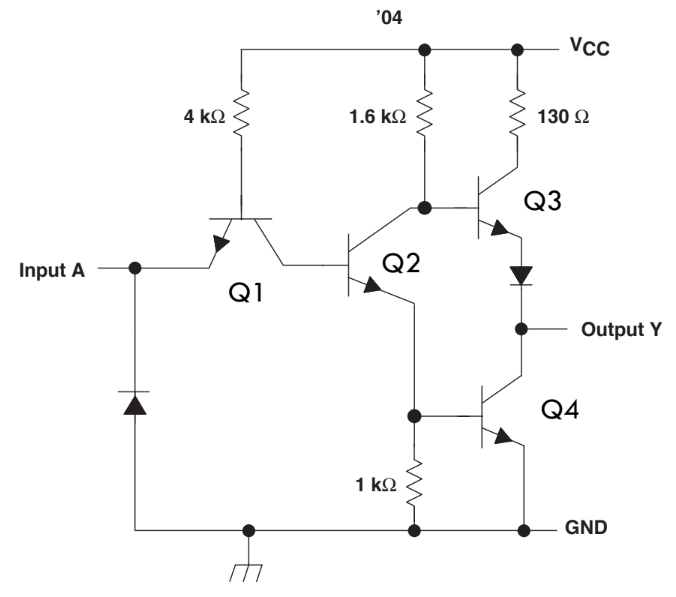
\includegraphics[scale=.5]{notttl}
	\caption{\sf{NOT} TTL.}
	\label{fig:notttl}
\end{figure}
Se l'input $A$ è scollegato, il transistor $Q_1$ è interdetto. Questo corrisponde a un segnale in ingresso alto ed è una caratteristica dei circuiti TTL: un ingresso scollegato è un ingresso a livello alto. Inoltre, $Q_2$ è accesso (perchè?), quindi anche $Q_4$ è acceso e dunque l'output è basso. Viceversa, se l'input $A$ è a livello basso $Q_1$ è acceso, quindi $Q_2$ e $Q_4$ sono spenti e l'uscita è alta. Tipicamente, in questa configurazione la corrente che scorre nel circuito è elevata, mentre con l'uscita alta tipicamente la corrente è quasi nulla. Il circuito TTL per un \sf{NAND} è in figura \ref{fig:nandttl}. In questo circuito compare un transistor con due emettitori. Magicamente, è sufficiente che uno dei due ingressi $A$ o $B$ sia basso per accendere $Q_1$, e dunque per avere un $Y$ basso.
\begin{figure}[h!]
	\centering
	\includegraphics[scale=.5]{nandttl}
	\caption{\sf{NAND} TTL.}
	\label{fig:nandttl}
\end{figure}
Si noti che in entrambi i circuiti sono presenti delle resistenze tra la tensione di alimentazione e i transistor. Queste resistenze sono dette di pull-up, valgono tipicamente $1-10\,\mathrm{k}\Omega$ e sono utilizzate per sopprimere oscillazioni e transizioni spurie del circuito, ma purtroppo aumentano il consumo quando la linea è bassa.

Come ultima cosa sui TTL, vediamo tre tipologie di circuiti di uscita in figura \ref{fig:uscitattl}. In particolare, un circuito tri-state è un circuito che ha tre livelli logici: gli usuali 0 e 1 e un livello indicato con $Z$, dove $Z$ è anche l'impedenza in uscita nello stato $Z$. Questo livello può essere usato per rimuovere "temporaneamente" la porta dal circuito. %MANCANO I MOS
\begin{figure}[h!]
	\centering
	\includegraphics[scale=.5]{uscitattl}
	\caption{tre tipologie di uscita TTL.}
	\label{fig:uscitattl}
\end{figure}

Vediamo ora qualche caratteristica generale dei circuiti logici. Abbiamo visto che il fan-out è il numero massimo di porte che possiamo collegare all'uscita di una data porta, senza alternarne il funzionamento. Queste porte in uscita sono di fatto in parallelo, quindi il fan-out $N$ è semplicemente
\[N=\frac{I_{OH}}{I_{IH}}\]
a patto che le porte in uscita siano tutte uguali. Qui $I_{OH}$ è la massima corrente erogabile in uscita dalla porta di cui vogliamo calcolare $N$, mentre $I_{IH}$ è la massima corrente in ingresso per le porte a valle. Sperimentalmente, il fan-out si può misurare collegando all'uscita di una data porta una resistenza variabile $R_L$ che simuli il carico di $N$ porte. L'altro capo di $R_L$ deve quindi andare a terra. In tal modo, quando l'uscita è alta possiamo stimare $I_{OH}$ (e poi che faccio?). Questa procedura può anche essere usata per stimare $I_{OL}$.%MANCA LA PARTE SUI TEMPI DI PROPAGAZIONE E SALITA


\subsection{Logica sequenziale}
Abbiamo già detto che nella logica sequenziale si considerano funzioni logiche la cui uscita può dipendere anche dagli stati precedenti del sistema. Intuitivamente possiamo quindi pensare a un loop di feedback che riporta l'uscita (o una sua parte) all'ingresso. Come vedremo, questo può anche portare a instabilità del sistema. Idealmente, vorremmo definire un tempo caratteristico $\Delta t$ del sistema per cui l'uscita $Z$ sia della forma
\[Z(t+\Delta t)=f(X(t), Z(t)\]
Questa equazione è detta equazione caratteristica. $\Delta t$ di fatto è uno stretto parente del tempo di propagazione, ma in genere non è chiaramente determinato, nel senso che dipende fortemente dal circuito considerato, dalle sue caratteristiche costruttive e tecnologiche, e anche dalle condizioni ambientali in cui opera.

Vediamo subito alcuni esempi di logica sequenziale. Consideriamo il circuito in figura \ref{fig:memory}. Questo circuito è un primo, rudimentale modello di memoria, nel senso che l'uscita è sempre allo stesso livello a ogni istante.
\begin{figure}[h!]
	\centering
	\begin{circuitikz}
		\draw(0,0)node[not port]{};
		\draw(2,0)node[not port]{};
		\draw(.5,0)to(1.4,0);
		\draw(-.7,0)to(-.7,1)to(3,1)to(3,0)to(3.5,0);
		\draw(2.5,0)to(3,0);
	\end{circuitikz}
	\caption{memory cell.}
	\label{fig:memory}
\end{figure}

A questo punto è facile implementare un meccanismo per la scrittura di un dato: basta infatti inserire due interrutori, in modo tale da interrompere il loop di feedback e chiudere l'interruttore in ingresso quando si vuole scrivere un dato, come in figura \ref{fig:memoryload}.
\begin{figure}[h!]
	\centering
	\begin{circuitikz}
		\draw(0,0)node[not port]{};
		\draw(2,0)node[not port]{};
		\draw(.5,0)to(1.4,0);
		\draw(-.7,0)to(-.7,1)to[switch](2,1)to(3,1)to(3,0)to(3.5,0);
		\draw(2.5,0)to(3,0);
		\draw(-2,0)to[switch](-0.7,0);
	\end{circuitikz}
	\caption{memory cell con meccanismo di scrittura.}
	\label{fig:memoryload}
\end{figure}
Il circuito mantiene questo tipo di funzionamento anche con un qualunque numero pari di porte \sf{NOT}. Viceversa, se abbiamo $N=2k+1$ porte \sf{NOT} in serie, e l'uscita dell'$N$-esima porta va all'entrata della prima porta, è facile vedere (ad esempio con una tabella di verità) che il circuito oscilla. Il periodo delle oscillazioni è
\[T=2N\Delta t\]
Un circuito di questo tipo si chiama ring oscillator.

Vediamo ora i latch, o flip flop. Questi circuiti sono circuiti sequenziali bistabili, che permettono di immagazzinare dati.
\subsubsection{$RS$ latch}
Un $RS$ latch è un miglioramento dei circuiti di memoria precedenti. L'implementazione consiste in due porte \sf{NOR} incrociate, come in figura \ref{fig:srlatch}.
\begin{figure}[h!]
	\centering
	\begin{circuitikz}
		\draw(0,1)node[nor port]{};
		\draw(0,-1)node[nor port]{};
		\draw(-1.5,1.28)node[anchor=east]{$R$}to(-1,1.28);
		\draw(0,1)to(1,1)node[anchor=west]{$Q$};
		\draw(0.5,1)to(.5,-0.1)to(-1.4,-.1)to(-1.4,-1+.28);
		\draw(-1.5,-1.28)node[anchor=east]{$S$}to(-1,-1.28);
		\draw(0,-1)to(1,-1)node[anchor=west]{$\overline Q$};
		\draw(0.3,0)to(.3,0.1)to(-1.4,.1)to(-1.4,1-.28);
		\draw(0.3,-1)to(0.3,-.2);
	\end{circuitikz}
	\caption{$RS$ latch.}
	\label{fig:srlatch}
\end{figure}
La "tabella di verità"\footnote{Una tabella di verità propriamente detta dovrebbe contenere anche i possibili valori di $Q(t)$, ma è molto meno di leggibile di quella mostrata qui.} associata è riportata in tabella \ref{tab:rslatch}.
\begin{table}[h!]
	\centering
	\begin{tabular}{c c |c c}
		$R(t)$&$S(t)$&$Q(t+\Delta t)$&$\overline{Q}(t+\Delta t)$\\\hline 0&0&$Q(t)$&$\overline{Q}(t)$\\0&1&1&0\\1&0&0&1\\1&1&0&0
	\end{tabular}
	\caption{tabella di verità per un $RS$ latch.}
	\label{tab:rslatch}
\end{table}
Da questa tabella capiamo che $R$ e $S$ stanno rispettivamente per reset e set. Inoltre, se $RS=00$ l'operazione fatta dal circuito è un hold, perchè mantiene in memoria il dato precedente. Infine, la configurazione $RS=11$ è da evitare, perchè corrisponde a situazioni non ammissibili in uscita, che porta in genere a oscillazioni non desiderabili in $Q$ e $\overline{Q}$. Uno strumento utile per capire il funzionamento del circuito è il diagramma di stato: in questo riportiamo dei cerchi che associamo agli stati possibili in uscita, e li colleghiamo con delle frecce corrispondenti alle possibili transizioni per dei valori dati di $R$ e $S$. Il diagramma di stato del $RS$ latch è riportato in figura \ref{fig:rslatchdiagstato}.
\begin{figure}[h!]
	\centering
	\includegraphics[scale=.5]{rslatch}
	\caption{diagramma di stato per $RS$ latch.}
	\label{fig:rslatchdiagstato}
\end{figure}
%SLIDE DELIRANTE SU CAMBIAMENTI BUFFI DI RS
Inoltre, dalla tabella di verità si deduce che l'equazione caratteristica del sistema è
\[Q(t+\Delta t)=S+\overline{R}\cdot Q(t)\]

Si può anche costruire un $RS$ latch con porte \sf{NAND}. Usualmente, questo circuito viene chiamato $\overline{RS}$ latch, perchè ha il set e il reset invertiti rispetto al $RS$ latch con porte \sf{NOR}, ossia sono scambiati e negati. Il circuito è in figura \ref{fig:rslatchnand} e la sua tabella di verità in figura \ref{tab:rslatchnand}
\begin{figure}[h!]
	\centering
	\begin{circuitikz}
		\draw(0,1)node[nand port]{};
		\draw(0,-1)node[nand port]{};
		\draw(-1.5,1.28)node[anchor=east]{$\overline{S}$}to(-1,1.28);
		\draw(0,1)to(1,1)node[anchor=west]{$Q$};
		\draw(0.5,1)to(.5,-0.1)to(-1.4,-.1)to(-1.4,-1+.28);
		\draw(-1.5,-1.28)node[anchor=east]{$\overline{R}$}to(-1,-1.28);
		\draw(0,-1)to(1,-1)node[anchor=west]{$\overline Q$};
		\draw(0.3,0)to(.3,0.1)to(-1.4,.1)to(-1.4,1-.28);
		\draw(0.3,-1)to(0.3,-.2);
	\end{circuitikz}
	\caption{$\overline{RS}$ latch.}
	\label{fig:rslatchand}
\end{figure}
\begin{table}[h!]
	\centering
	\begin{tabular}{c c |c c}
		$R(t)$&$S(t)$&$Q(t+\Delta t)$&$\overline{Q}(t+\Delta t)$\\\hline 0&0&$Q(t)$&$\overline{Q}(t)$\\0&1&1&0\\1&0&0&1\\1&1&0&0
	\end{tabular}
	\caption{tabella di verità per un $\overline{RS}$ latch.}
	\label{tab:rslatchnand}
\end{table}

Con lo scambio e la negazione di $R$ e $S$ l'equazione caratteristica e il funzionamento del circuito non cambiano.
\subsection{Enable e controllo del feedback}
Vediamo ora come implementare i due interruttori che in precedenza avevamo usato per permettere a una memoria di memorizzare nuovi dati. L'idea è semplice: si parte da un $RS$ latch e a monte di questo si mettono due \sf{NOR}, come mostrato in figura \ref{fig:gatedrslatch}. Il segnale $E$ è detto enable e gioca il ruolo di interruttore (anzi, di entrambi gli interruttori: questo è buono perchè vanno azionati contemporaneamente).
\begin{figure}[h!]
	\centering
	\begin{circuitikz}
		\draw(0,1)node[nor port]{};
		\draw(0,-1)node[nor port]{};
		\draw(-2,1.28)node[anchor=south]{${R}$}to(-1,1.28);
		\draw(0,1)to(1,1)node[anchor=west]{$Q$};
		\draw(0.5,1)to(.5,-0.1)to(-1.4,-.1)to(-1.4,-1+.28);
		\draw(-2,-1.28)node[anchor=north]{${S}$}to(-1,-1.28);
		\draw(0,-1)to(1,-1)node[anchor=west]{$\overline Q$};
		\draw(0.3,0)to(.3,0.1)to(-1.4,.1)to(-1.4,1-.28);
		\draw(0.3,-1)to(0.3,-.2);
		\draw(-2,1.28)node[nor port]{};
		\draw(-2,-1.28)node[nor port]{};
		\draw(-4,1.28+.28)node[anchor=east]{$\overline{R}$}to(-3,1.28+.28);
		\draw(-4,-1.28-.28)node[anchor=east]{$\overline{S}$}to(-3,-1.28-.28);
		\draw(-4,0)node[anchor=east]{$\overline{E}$}to(-3.4,0);
		\draw(-3.4,1)to(-3.4,-1);
	\end{circuitikz}
	\caption{${RS}$ latch con enable.}
	\label{fig:gatedrslatch}
\end{figure}
Lo stesso si può fare con un $\overline{RS}$ latch, semplicemente usando porte \sf{NAND} al posto di porte \sf{NOR}. In tal caso, si aggiungono anche un preset $PR$ e un cleare $CL$, ossia si sostistuiscono i \sf{NAND} del $\overline{RS}$ latch con \sf{NAND} a tre ingressi, in cui il terzo ingresso è $PR$ oppure $CL$. In condizioni normali entrambi i segnali sono alti, quindi per ora non ce ne preoccupiamo.

L'enable può anche essere collegato a un clock, in maniera tale da sincronizzare le operazioni di transizione del circuito. Ad esempio, come clock possiamo usare un OpAmp in regime non lineare. La tabella di verità del sistema è riportata in tabella \ref{tab:gatedrslatch}.
\begin{table}[h!]
	\centering
	\begin{tabular}{c|c c|c c|c c}
		$E$&$\overline{R}$&$\overline{S}$&$R$&$S$&$Q(t+\Delta t)$&$\overline{Q}(t+\Delta t)$\\\hline
		0&X&X&X&X&$Q(t)$&$\overline{Q}(t)$\\1&1&1&0&0&$Q(t)$&$\overline{Q}(t)$\\1&1&0&0&1&1&0\\1&0&1&1&0&0&1\\1&0&0&1&1&0&0
	\end{tabular}
	\caption{tabella di verità per un $RS$ latch con enable.}
	\label{tab:gatedrslatch}
\end{table}
Come anticipato, se $E=0$ il circuito è in hold, qualunque siano $\overline{R}$ e $\overline{S}$. Viceversa, se $E=1$ recuperiamo l'usuale $RS$ latch, compresa la fastidiosa oscillazione per $RS=11$. Questo problema viene risolto nella sezione successiva.
\subsubsection{$D$ latch}
Rappresentiamo ora con un quadrato un $RS$ latch. Un $D$ latch si ottiene mandando un segnale $D$ alla porta $R$ e il suo negato $\overline{D}$ alla porta $S$. Il circuito è quindi quello di figura \ref{fig:dlatch}. Abbiamo anche aggiunto un clock $CK$, da collegare all'enable $E$ del $RS$ latch.
\begin{figure}[h!]
	\centering
	\begin{circuitikz}
		\draw(0,.5)to(2,.5)to(2,-1.5)to(0,-1.5)to(0,0.5);
		\draw(-3,0)node[anchor=east]{$D$}to(0,0)node[anchor=west]{$R$};
		\draw(-1,-1)to(0,-1)node[anchor=west]{$S$};
		\draw(-2.3,-1)to(-2.3,0);
		\draw(-1.6,-1)node[not port]{};
		\draw(1,-1.5)node[anchor=south]{$E$}to(1,-2)node[anchor=north]{$CK$};
		\draw(2,0)node[anchor=east]{$Q$}to(3,0);
		\draw(2,-1)node[anchor=east]{$\overline Q$}to(3,-1);
		\end{circuitikz}
	\caption{$D$ latch.}
	\label{fig:dlatch}
\end{figure}

La tabella di verità è quella in tabella \ref{tab:dlatch}. Si noti che non è possibile avere $RS=11$, ma neanche $RS=00$. Effettivamente lo stato del sistema al tempo $t+\Delta t$ non dipende più dallo stato al tempo $t$ in nessuna configurazione, quindi si parla di transparent latch.
\begin{table}[h!]
	\centering
	\begin{tabular}{c|cc|cc}
		$D$&$R$&$S$&$Q(t+\Delta t)$&$\overline{Q}(t+\Delta t)$\\\hline1&0&1&1&0\\0&1&0&0&1
	\end{tabular}
	\caption{tabella di verità per un $D$ latch.}
	\label{tab:dlatch}
\end{table}
Il diagramma degli stati del $D$ latch è riportato in figura \ref{fig:dlatchdiagstati}
\begin{figure}[h!]
	\centering
	\includegraphics[scale=0.5]{dlatch}
	\caption{diagramma degli stati di un $D$ latch.}
	\label{fig:dlatchdiagstati}
\end{figure}
(Qua dicono che il dato $D$ viene trasferito quando il clock passa a livello alto. Una volta diventato alto, le uscite non risentono di eventuali variazioni di $D$ fino al prossimo impulso di clock, dunque si ha un meccanismo di edge triggering. A me sembra falso se il clock è l'enable precedente).
\subsubsection{$JK$ latch}
Il $JK$ latch rappresenta un'altra possibile soluzione al problema $RS=11$, e in più permette di avere l'hold e una nuova funzione chiamata toggle. Il circuito è riportato in figura \ref{fig:jklatch}.
\begin{figure}[h!]
	\centering
	\begin{circuitikz}
		\draw(0,.5)to(2,.5)to(2,-1.5)to(0,-1.5)to(0,0.5);
		\draw(-1,0.25)node[nand port]{}to(0,0.25)node[anchor=west]{$R$};
		\draw(-1,-1.25)node[nand port]{}to(0,-1.25)node[anchor=west]{$S$};
		\draw(-2.4,.25-.28)node[anchor=east]{$J$};
		\draw(-2.4,-1.25+.28)node[anchor=east]{$K$};
		\draw(-2.4,.25+.28)to(-2.4,1)to(2.2,1)to(2.2,0.1);
		\draw(2.2,-.1)to(2.2,-1);
		\draw(-2.4,-1.25-.28)to(-2.4,-2)to(2.6,-2)to(2.6,-1.1);
		\draw(2.6,-.9)to(2.6,0);
		\draw(0,-.5)node[anchor=west]{$E$}to(-.5,-.5)node[anchor=east]{$CK$};
		\draw(2,0)node[anchor=east]{$Q$}to(3,0);
		\draw(2,-1)node[anchor=east]{$\overline Q$}to(3,-1);
	\end{circuitikz}
	\caption{$JK$ latch.}
	\label{fig:jklatch}
\end{figure}
La tabella di verità estesa è riportata in tabella \ref{tab:jklatch}.
\begin{table}[h!]
	\centering
	\begin{tabular}{c|c c| c c| c c}
		$Q(t)$&$J$&$K$&$R$&$S$&$Q(t+\Delta t)$&$\overline{Q}(t+\Delta t)$\\\hline X&0&0&0&0&$Q(t)$&$\overline{Q}(t+\Delta t)$\\1&1&0&0&0&1&0\\0&1&0&1&0&1&0\\1&0&1&0&1&0&1\\0&0&1&0&0&0&1\\1&1&1&0&1&0&1\\0&1&1&1&0&1&0
	\end{tabular}
	\caption{tabella di verità per un $JK$ latch.}
	\label{tab:jklatch}
\end{table}

Cioè se $JK=00$ il sistema è in hold, se $JK=10$ il sistema è in set, se $JK=01$ il sistema è in reset, mentre se $JK=11$ il sistema è in toggle: l'uscita al tempo $t+\Delta t$ è la complementare dell'uscita al tempo $t$. La tabella di verità è quindi riassumibile con quella in tabella \ref{tab:shortjk}.
\begin{table}[h!]
	\centering
	\begin{tabular}{c c| c c| c c}
		$J$&$K$&$R$&$S$&$Q(t+\Delta t)$&$\overline{Q}(t+\Delta t)$\\\hline 0&0&0&0&$Q(t)$&$\overline{Q}(t+\Delta t)$\\1&0&0&0&1&0\\0&1&0&1&0&1\\1&1&0&1&$\overline{Q}(t)$&$Q(t)$
	\end{tabular}
	\caption{tabella di verità per un $JK$ latch.}
	\label{tab:shortjk}
\end{table}
Inoltre, il diagramma degli stati è in figura \ref{fig:jklatchdiagstati}.
\begin{figure}[h!]
	\centering
	\includegraphics[scale=0.5]{jklatch}
	\caption{diagramma degli stati di un $JK$ latch.}
	\label{fig:jklatchdiagstati}
\end{figure}
Supponiamo ora che sia $JK=11$. Se $t_C$ è il tempo in cui il segnale di clock è alto e $t_P$ il tempo di propagazione del sistema, se $t_P\ll t_C$ (ossia se il sistema è molto reattivo) $Q$ comincia a oscillare, ossia va in race around condition. Il problema viene risolto nella prossima sezione
\subsubsection{Dispositivi level-sensitive e edge-sensitive}
L'idea per evitare la race around condition è costruire dei circuiti con un clock che siano edge-sensitive piuttosto che level-sensitive: nei circuiti precendenti le transizioni erano possibili ogni volta che $CK=1$, mentre ora vorremmo costruire dei sistemi in cui le transizioni siano possibili solo in un piccolo intervallo temporale intorno alla transizione $CK=1\rightarrow CK=0$ o viceversa. Un primo circuito in cui è possibile fare ciò è un circuito di tipo master-slave. In questo tipo di circuito abbiamo due latch. Un unico clock va alle porte enable dei due latch, ma viene negato prima di entrare in uno dei due latch. Inoltre, il segnale di input viene mandato al latch denominato master, il cui output è collegato all'input del secondo latch, chiamato slave. In tal modo, sia il master che lo slave sono abilitati solo per metà di un periodo del clock, e mai contemporaneamente. Ad esempio, in figura \ref{fig:masterslavers} è riportato un $RS$ flip-flop master-slave.
\begin{figure}[h!]
	\centering
	\begin{circuitikz}
		\draw(0,.5)to(2,.5)to(2,-1.5)to(0,-1.5)to(0,0.5);
		\draw(-1,0)node[anchor=east]{$R$}to(0,0)node[anchor=west]{$R_1$};
		\draw(-1,-1)node[anchor=east]{$S$}to(0,-1)node[anchor=west]{$S_1$};
		\draw(0,-.5)node[anchor=west]{$E_1$}to(-1,-.5)node[anchor=east]{$CK$};
		\draw(2,0)node[anchor=east]{$Q_1$}to(3,0)node[anchor=west]{$R_2$};
		\draw(2,-1)node[anchor=east]{$\overline Q_1$}to(3,-1)node[anchor=west]{$S_2$};
		\draw(3,.5)to(5,.5)to(5,-1.5)to(3,-1.5)to(3,0.5);
		\draw(5,0)node[anchor=east]{$Q_1$}to(6,0)node[anchor=west]{$Q$};
		\draw(5,-1)node[anchor=east]{$\overline Q_2$}to(6,-1)node[anchor=west]{$\overline{Q}$};
		\draw(-.5,-.5)to(-.5,-.9);
		\draw(-.5,-1.1)to(-.5,-2.5)to(1.3,-2.5);
		\draw(1.8,-2.5)node[not port]{};
		\draw(2.5,-2.5)to(2.5,-2.5)to(2.5,-1.1);
		\draw(2.5,-.9)to(2.5,-.5)to(3,-.5)node[anchor=west]{$E_2$};
	\end{circuitikz}
	\caption{master-slave $RS$.}
	\label{fig:masterslavers}
\end{figure}
%DELIRIO SU 1s CATCHING PROBLEM.
Chiaramente, è possibile creare anche dei flip-flop con master slave di tipo $JK$ e $D$, è sufficiente sostituire i latch nelle implementazioni precedenti con due latch. Le due implementazioni sono in figura \ref{fig:masterslavejk} e \ref{fig:masterslaved}
\begin{figure}[h!]
	\centering
	\begin{circuitikz}
		\draw(0,.5)to(2,.5)to(2,-1.5)to(0,-1.5)to(0,0.5);
		\draw(-3,0)node[anchor=east]{$D$}to(0,0)node[anchor=west]{$R_1$};
		\draw(-1,-1)to(0,-1)node[anchor=west]{$S_1$};
		\draw(-1.5,-1)node[not port]{};
		\draw(-2.5,0)to(-2.5,-1)to(-2.2,-1);
		\draw(0,-.5)node[anchor=west]{$E_1$}to(-1,-.5)node[anchor=east]{$CK$};
		\draw(2,0)node[anchor=east]{$Q_1$}to(3,0)node[anchor=west]{$R_2$};
		\draw(2,-1)node[anchor=east]{$\overline Q_1$}to(3,-1)node[anchor=west]{$S_2$};
		\draw(3,.5)to(5,.5)to(5,-1.5)to(3,-1.5)to(3,0.5);
		\draw(5,0)node[anchor=east]{$Q_1$}to(6,0)node[anchor=west]{$Q$};
		\draw(5,-1)node[anchor=east]{$\overline Q_2$}to(6,-1)node[anchor=west]{$\overline{Q}$};
		\draw(-.5,-.5)to(-.5,-.9);
		\draw(-.5,-1.1)to(-.5,-2.5)to(1.3,-2.5);
		\draw(1.8,-2.5)node[not port]{};
		\draw(2.5,-2.5)to(2.5,-2.5)to(2.5,-1.1);
		\draw(2.5,-.9)to(2.5,-.5)to(3,-.5)node[anchor=west]{$E_2$};
	\end{circuitikz}
	\caption{master-slave $D$.}
	\label{fig:masterslaved}
\end{figure}
\begin{figure}[h!]
	\centering
	\begin{circuitikz}
		\draw(0,.5)to(2,.5)to(2,-1.5)to(0,-1.5)to(0,0.5);
		\draw(-1,0.25)node[nand port]{}to(0,0.25)node[anchor=west]{$R_1$};
		\draw(-1,-1.25)node[nand port]{}to(0,-1.25)node[anchor=west]{$S_1$};
		\draw(0,-.5)node[anchor=west]{$E_1$}to(-1,-.5)node[anchor=east]{$CK$};
		\draw(2,0)node[anchor=east]{$Q_1$}to(3,0)node[anchor=west]{$R_2$};
		\draw(2,-1)node[anchor=east]{$\overline Q_1$}to(3,-1)node[anchor=west]{$S_2$};
		\draw(3,.5)to(5,.5)to(5,-1.5)to(3,-1.5)to(3,0.5);
		\draw(5,0)node[anchor=east]{$Q_1$}to(6,0)node[anchor=west]{$Q$};
		\draw(5,-1)node[anchor=east]{$\overline Q_2$}to(6,-1)node[anchor=west]{$\overline{Q}$};
		\draw(-.5,-.5)to(-.5,-.9);
		\draw(-.5,-1.1)to(-.5,-2.5)to(1.3,-2.5);
		\draw(1.8,-2.5)node[not port]{};
		\draw(2.5,-2.5)to(2.5,-2.5)to(2.5,-1.1);
		\draw(2.5,-.9)to(2.5,-.5)to(3,-.5)node[anchor=west]{$E_2$};
		\draw(-2.4,.25-.28)node[anchor=east]{$J$};
		\draw(-2.4,-1.25+.28)node[anchor=east]{$K$};
		\draw(-2.4,.25+.28)to(-2.4,1)to(5.3,1)to(5.3,.1);
		\draw(5.3,-.1)to(5.3,-1);
		\draw(-2.4,-1.25-.28)to(-2.4,-2)to(5.6,-2)to(5.6,-1.1);
		\draw(5.6,-.9)to(5.6,0);
	\end{circuitikz}
	\caption{master-slave $JK$.}
	\label{fig:masterslavejk}
\end{figure}
%QUI C'E' TUTTA LA ZOOLOGIA DI LATCH, FLIP FLOP E MASTER SLAVE CHE ORA NON HO VOGLIA DI FARE.
\subsubsection{Contatori}
\end{document}